% ====================================================================
%  徐森林、金亚东、薛春华《数学分析》（第三册）
%  第 16 章  Fourier 分析
%  源：原书印刷页 244-308（PDF 物理页 = 印刷页 + 6）
% ====================================================================

\chapter{Fourier 分析}\label{ch:16}

在第 14 章中已详细讨论了一种特殊的函数项级数——幂级数, 它的每一项都是幂函数. 这一章我们要讨论另一种特殊的函数项级数——三角级数:
\[
  \sum_{n=0}^{\infty}(a_{n}\cos nx+b_{n}\sin nx),
\]
它的每一项都是三角函数. 这种级数有强烈的物理背景, 它是工程技术, 特别是无线电、通信、数字处理中一个不可缺少的重要数学工具.

我们先证 Fourier 级数的收敛定理, 然后列举大量函数的 Fourier 级数的展开式, 有时取特殊点代入获得意想不到的数项级数的值. 接着引进了平方平均收敛的重要概念, 证明了 Bessel 不等式与 Parseval 等式.

Fourier 变换是数学物理中一种重要的积分变换, 它能将分析运算转化为代数运算, 从而使问题大大简化, 它与 Fourier 级数密切相关, 并有广泛的应用价值.

为了使一类条件更弱更广泛的函数有 Fourier 展开式, 我们将修改传统的收敛概念, 引进 Cas`aro 求和的重要定义, 并建立相应的一套理论.

% ====================================================================
%  徐森林、金亚东、薛春华《数学分析》（第三册）
%  第 16 章  Fourier 分析
%  §16.1  周期函数的 Fourier 级数及收敛定理 (PART-A)
%  源：原书印刷页 244-256（PDF 物理页 250-262）
% ====================================================================

\section{周期函数的 Fourier 级数及收敛定理}\label{sec:16.1}

设 $g(t)$ 是以 $T\neq 0$ 为周期的周期函数, 即 $g(t+T)=g(t)$, 作变量代换
\[
  x=\frac{2\pi}{T}t\quad\text{或}\quad t=\frac{T}{2\pi}x,
\]
就有
\[
  g(t)=g\left(\frac{T}{2\pi}x\right)=f(x).
\]
于是, $f(x)$ 就是以 $2\pi$ 为周期的周期函数. 因此, 只需讨论以 $2\pi$ 为周期的周期函数. 设 $f(x)$ 是以 $2\pi$ 为周期的周期函数, 自然会问, 在什么条件下, $f(x)$ 能表示为
\[
  f(x)=\frac{a_{0}}{2}+\sum_{n=1}^{\infty}(a_{n}\cos nx+b_{n}\sin nx).
\]
此外, 如何确定系数 $a_{0}, a_{n}, b_{n}$ ($n=1,2,\cdots$).

\begin{theorem}\label{thm:16.1.1}
设以 $2\pi$ 为周期的周期函数 $f(x)$ 可表示为
\[
  f(x)=\frac{a_{0}}{2}+\sum_{n=1}^{\infty}(a_{n}\cos nx+b_{n}\sin nx).
\]
如果上述级数在 $[-\pi,\pi]$ 上一致收敛于 $f(x)$, 则
\[
  \left\{\begin{aligned}
    a_{n}&=\frac{1}{\pi}\int_{-\pi}^{\pi}f(x)\cos nx\,\mathrm{d}x,\quad n=0,1,2,\cdots,\\
    b_{n}&=\frac{1}{\pi}\int_{-\pi}^{\pi}f(x)\sin nx\,\mathrm{d}x,\quad n=1,2,\cdots.
  \end{aligned}\right.
\]
\end{theorem}

\begin{proof}
因为 $\displaystyle\frac{a_{0}}{2}+\sum_{n=1}^{\infty}(a_{n}\cos nx+b_{n}\sin nx)$ 在 $[-\pi,\pi]$ 上一致收敛于 $f(x)$, 根据函数项级数一致收敛的 Cauchy 准则知,
\[
  \frac{a_{0}}{2}\cos nx+\sum_{k=1}^{\infty}(a_{k}\cos kx\cos nx+b_{k}\sin kx\cos nx)
\]
在 $[-\pi,\pi]$ 上一致收敛于 $f(x)\cos nx$. 应用逐项积分的定理~\ref{thm:13.2.3p}得到
\[
  \begin{aligned}
    \int_{-\pi}^{\pi}f(x)\cos nx\,\mathrm{d}x&=\frac{a_{0}}{2}\int_{-\pi}^{\pi}\cos nx\,\mathrm{d}x\\
    &\quad+\sum_{k=1}^{\infty}\left(a_{k}\int_{-\pi}^{\pi}\cos kx\cos nx\,\mathrm{d}x+b_{k}\int_{-\pi}^{\pi}\sin kx\cos nx\,\mathrm{d}x\right)\\
    &\xlongequal{\text{\extref{例 6.3.3}}}\frac{a_{0}}{2}\cdot 2\pi\delta_{0n}+\sum_{k=1}^{\infty}(a_{k}\cdot\pi\delta_{kn}+b_{k}\cdot 0)=\pi a_{n},\quad n=0,1,2,\cdots,
  \end{aligned}
\]
其中
\[
  \delta_{kn}=\begin{cases}
    1, & k=n,\\
    0, & k\neq n.
\end{cases}
\]
同理, 有
\[
  \begin{aligned}
    \int_{-\pi}^{\pi}f(x)\sin nx\,\mathrm{d}x&=\frac{a_{0}}{2}\int_{-\pi}^{\pi}\sin nx\,\mathrm{d}x\\
    &\quad+\sum_{k=1}^{\infty}\left(a_{k}\int_{-\pi}^{\pi}\cos kx\sin nx\,\mathrm{d}x+b_{k}\int_{-\pi}^{\pi}\sin kx\sin nx\,\mathrm{d}x\right)\\
    &\xlongequal{\text{\extref{例 6.3.3}}}\frac{a_{0}}{2}\cdot 0+\sum_{k=1}^{\infty}(a_{k}\cdot 0+b_{k}\cdot\pi\delta_{kn})=\pi b_{n},\quad n=1,2,\cdots.
  \end{aligned}
\]
于是得到
\[
  \left\{\begin{aligned}
    a_{n}&=\frac{1}{\pi}\int_{-\pi}^{\pi}f(x)\cos nx\,\mathrm{d}x,\quad n=0,1,2,\cdots,\\
    b_{n}&=\frac{1}{\pi}\int_{-\pi}^{\pi}f(x)\sin nx\,\mathrm{d}x,\quad n=1,2,\cdots.
  \end{aligned}\right.
\]
\end{proof}

\begin{definition}\label{def:16.1.1}
设 $f(x)$ 是周期为 $2\pi$ 的函数, 它在 $[-\pi,\pi]$ 上可积或绝对可积 (如果 $f(x)$ 是有界函数, 就假定它是 Riemann 可积的, 简称可积; 如果 $f(x)$ 是无界函数, 就假定它是广义绝对可积的, 简称绝对可积). 称由公式
\[
  \left\{\begin{aligned}
    a_{n}&=\frac{1}{\pi}\int_{-\pi}^{\pi}f(x)\cos nx\,\mathrm{d}x,\quad n=0,1,2,\cdots,\\
    b_{n}&=\frac{1}{\pi}\int_{-\pi}^{\pi}f(x)\sin nx\,\mathrm{d}x,\quad n=1,2,\cdots
  \end{aligned}\right.
\]
确定的 $a_{n}, b_{n}$ 为 $f(x)$ 的 \textbf{Fourier 系数}, 由 $a_{n}, b_{n}$ 确定的级数
\[
  \frac{a_{0}}{2}+\sum_{n=1}^{\infty}(a_{n}\cos nx+b_{n}\sin nx)
\]
称为 $f(x)$ 的 \textbf{Fourier 级数}, 记为
\[
  f(x)\sim\frac{a_{0}}{2}+\sum_{n=1}^{\infty}(a_{n}\cos nx+b_{n}\sin nx).
\]
\end{definition}

至于这个级数是否收敛, 如果收敛的话, 它的和是否就等于 $f(x)$, 这些问题都有待进一步研究. 但有一点是可以肯定的, 这个级数是由 $f(x)$ 确定的.

在推论~\ref{cor:16.1.3}中将看到, 对于相当广泛的一类函数, 它的 Fourier 级数是收敛于它自己的, 这正是 Fourier 级数所以重要的原因.

\begin{theorem}[Riemann-Lebesgue 引理]\label{thm:16.1.2}
设 $f(x)$ 在 $[a,b]$ 上可积或绝对可积, 则
\[
  \lim_{\lambda\to+\infty}\int_{a}^{b}f(x)\cos\lambda x\,\mathrm{d}x=0,\quad \lim_{\lambda\to+\infty}\int_{a}^{b}f(x)\sin\lambda x\,\mathrm{d}x=0.
\]
\end{theorem}

\begin{proof}
只证第一个等式, 第二个等式的证明完全类似.

\textbf{情形 1: $f(x)$ 在 $[a,b]$ 上有连续导数.}

此时, 应用分部积分公式, 有
\[
  \begin{aligned}
    \left|\int_{a}^{b}f(x)\cos\lambda x\,\mathrm{d}x\right|&=\left|\frac{1}{\lambda}\left(\left.f(x)\sin\lambda x\right|_{a}^{b}-\int_{a}^{b}f'(x)\sin\lambda x\,\mathrm{d}x\right)\right|\\
    &\leqslant\frac{1}{\lambda}\left(|f(b)|+|f(a)|+\int_{a}^{b}|f'(x)|\,\mathrm{d}x\right)\to 0\quad(\lambda\to+\infty).
  \end{aligned}
\]

\textbf{情形 2: $f(x)$ 在 $[a,b]$ 上可积.}

由\extref{定理 6.2.2}知, $\forall\varepsilon>0$, 存在连续函数 $g(x)$, 使得
\[
  \int_{a}^{b}|f(x)-g(x)|\,\mathrm{d}x<\frac{\varepsilon}{3}.
\]
再由 Weierstrass 多项式逼近定理 (\extref{定理 13.2.8}) 知, 存在多项式 $P(x)$, 使得
\[
  \max_{x\in[a,b]}|g(x)-P(x)|<\frac{\varepsilon}{3(b-a)}.
\]
于是,
\[
  \int_{a}^{b}|g(x)-P(x)|\,\mathrm{d}x<\frac{\varepsilon}{3}.
\]
由情形 1 知, 存在 $\Lambda>0$, 当 $\lambda>\Lambda$ 时,
\[
  \left|\int_{a}^{b}P(x)\cos\lambda x\,\mathrm{d}x\right|<\frac{\varepsilon}{3}.
\]
因此, 当 $\lambda>\Lambda$ 时,
\[
  \begin{aligned}
    \left|\int_{a}^{b}f(x)\cos\lambda x\,\mathrm{d}x\right|&\leqslant\int_{a}^{b}|f(x)-g(x)|\,\mathrm{d}x+\int_{a}^{b}|g(x)-P(x)|\,\mathrm{d}x+\left|\int_{a}^{b}P(x)\cos\lambda x\,\mathrm{d}x\right|\\
    &<\frac{\varepsilon}{3}+\frac{\varepsilon}{3}+\frac{\varepsilon}{3}=\varepsilon.
  \end{aligned}
\]

\textbf{情形 3: $f(x)$ 在 $[a,b]$ 上绝对可积.}

假定无界点在端点 $a$ (对于有限个无界点, 或无界点在区间内部的情形, 可分段化为此种情形). 由广义绝对可积的定义知, $\forall\varepsilon>0$, 存在 $a'>a$, 使得
\[
  \int_{a}^{a'}|f(x)|\,\mathrm{d}x<\frac{\varepsilon}{2}.
\]
因为 $f(x)$ 在 $[a',b]$ 上可积, 由情形 2 知, 存在 $\Lambda>0$, 当 $\lambda>\Lambda$ 时,
\[
  \left|\int_{a'}^{b}f(x)\cos\lambda x\,\mathrm{d}x\right|<\frac{\varepsilon}{2}.
\]
从而, 当 $\lambda>\Lambda$ 时,
\[
  \left|\int_{a}^{b}f(x)\cos\lambda x\,\mathrm{d}x\right|\leqslant\int_{a}^{a'}|f(x)|\,\mathrm{d}x+\left|\int_{a'}^{b}f(x)\cos\lambda x\,\mathrm{d}x\right|<\frac{\varepsilon}{2}+\frac{\varepsilon}{2}=\varepsilon.
\]
\end{proof}

\begin{theorem}\label{thm:16.1.3}
设 $\{a_{n}\}, \{b_{n}\}$ 为可积或绝对可积函数的 Fourier 系数序列, 则
\[
  \lim_{n\to+\infty}a_{n}=0,\quad \lim_{n\to+\infty}b_{n}=0.
\]
\end{theorem}

\begin{proof}
直接由定理~\ref{thm:16.1.2} (取 $[a,b]=[-\pi,\pi]$, $\lambda=n$) 即得.
\end{proof}

\begin{remark}\label{rem:16.1.1}
如果 $\lim\limits_{n\to+\infty}a_{n}\neq 0$ 或 $\lim\limits_{n\to+\infty}b_{n}\neq 0$, 则三角级数 $\displaystyle\frac{a_{0}}{2}+\sum_{n=1}^{\infty}(a_{n}\cos nx+b_{n}\sin nx)$ 一定不是任何可积或绝对可积函数的 Fourier 级数.
\end{remark}

\begin{theorem}\label{thm:16.1.4}
设 $f(x)$ 在 $[-\pi,\pi]$ 上连续, $f(-\pi)=f(\pi)$, 且有可积或绝对可积的导函数 $f'(x)$, 则
\[
  a_{n}=o\left(\frac{1}{n}\right),\quad b_{n}=o\left(\frac{1}{n}\right)\quad(n\to+\infty).
\]
\end{theorem}

\begin{proof}
应用分部积分公式,
\[
  \begin{aligned}
    a_{n}&=\frac{1}{\pi}\int_{-\pi}^{\pi}f(x)\cos nx\,\mathrm{d}x=\frac{1}{n\pi}\left(\left.f(x)\sin nx\right|_{-\pi}^{\pi}-\int_{-\pi}^{\pi}f'(x)\sin nx\,\mathrm{d}x\right)\\
    &=-\frac{1}{n\pi}\int_{-\pi}^{\pi}f'(x)\sin nx\,\mathrm{d}x.
  \end{aligned}
\]
由定理~\ref{thm:16.1.2}知, $\lim\limits_{n\to+\infty}\displaystyle\frac{1}{\pi}\int_{-\pi}^{\pi}f'(x)\sin nx\,\mathrm{d}x=0$, 故 $a_{n}=o\left(\frac{1}{n}\right)$.

同理,
\[
  \begin{aligned}
    b_{n}&=\frac{1}{\pi}\int_{-\pi}^{\pi}f(x)\sin nx\,\mathrm{d}x=\frac{1}{n\pi}\left(-\left.f(x)\cos nx\right|_{-\pi}^{\pi}+\int_{-\pi}^{\pi}f'(x)\cos nx\,\mathrm{d}x\right)\\
    &=\frac{1}{n\pi}\left[-(-1)^{n}(f(\pi)-f(-\pi))+\int_{-\pi}^{\pi}f'(x)\cos nx\,\mathrm{d}x\right]=\frac{1}{n\pi}\int_{-\pi}^{\pi}f'(x)\cos nx\,\mathrm{d}x=o\left(\frac{1}{n}\right).
  \end{aligned}
\]
\end{proof}

\begin{theorem}\label{thm:16.1.5}
设 $f(x)$ 在 $[-\pi,\pi]$ 上有直到 $k+1$ 阶导数, $f^{(k+1)}(x)$ 可积或绝对可积, 且
\[
  f^{(j)}(-\pi)=f^{(j)}(\pi),\quad j=0,1,\cdots,k-1,
\]
则
\[
  a_{n}=o\left(\frac{1}{n^{k+1}}\right),\quad b_{n}=o\left(\frac{1}{n^{k+1}}\right)\quad(n\to+\infty).
\]
\end{theorem}

\begin{proof}
连续应用 $k+1$ 次分部积分法, 并利用边界条件 $f^{(j)}(-\pi)=f^{(j)}(\pi)$ ($j=0,1,\cdots,k-1$), 即化为 $f^{(k+1)}(x)$ 的 Fourier 系数除以 $n^{k+1}$, 再由定理~\ref{thm:16.1.2}知结论成立.
\end{proof}

设 $f(x)$ 是周期为 $2\pi$ 的函数, 在 $[-\pi,\pi]$ 上可积或绝对可积. 记它的 Fourier 级数的部分和为
\[
  S_{n}(x)=\frac{a_{0}}{2}+\sum_{k=1}^{n}(a_{k}\cos kx+b_{k}\sin kx).
\]
将系数 $a_{k}, b_{k}$ 的积分表达式代入, 得到
\[
  \begin{aligned}
    S_{n}(x_{0})&=\frac{1}{2\pi}\int_{-\pi}^{\pi}f(x)\,\mathrm{d}x+\sum_{k=1}^{n}\left(\frac{1}{\pi}\int_{-\pi}^{\pi}f(x)\cos kx\cos kx_{0}\,\mathrm{d}x+\frac{1}{\pi}\int_{-\pi}^{\pi}f(x)\sin kx\sin kx_{0}\,\mathrm{d}x\right)\\
    &=\frac{1}{\pi}\int_{-\pi}^{\pi}f(x)\left[\frac{1}{2}+\sum_{k=1}^{n}\cos k(x-x_{0})\right]\mathrm{d}x=\frac{1}{\pi}\int_{-\pi}^{\pi}f(x)\frac{\sin\left(n+\frac{1}{2}\right)(x-x_{0})}{2\sin\frac{x-x_{0}}{2}}\,\mathrm{d}x\\
    &\xlongequal{\text{\extref{例 6.4.9}(3)}}\frac{1}{\pi}\int_{x_{0}-\pi}^{x_{0}+\pi}f(x)\frac{\sin\left(n+\frac{1}{2}\right)(x-x_{0})}{2\sin\frac{x-x_{0}}{2}}\,\mathrm{d}x\\
    &\xlongequal{t=x-x_{0}}\frac{1}{\pi}\int_{-\pi}^{\pi}f(t+x_{0})\frac{\sin\left(n+\frac{1}{2}\right)t}{2\sin\frac{t}{2}}\,\mathrm{d}t\\
    &\xlongequal{t=-u}\frac{1}{\pi}\int_{0}^{\pi}f(x_{0}+t)\frac{\sin\left(n+\frac{1}{2}\right)t}{2\sin\frac{t}{2}}\,\mathrm{d}t+\frac{1}{\pi}\int_{0}^{\pi}f(x_{0}-u)\frac{\sin\left(n+\frac{1}{2}\right)u}{2\sin\frac{u}{2}}\,\mathrm{d}u\\
    &=\frac{1}{\pi}\int_{0}^{\pi}[f(x_{0}+t)+f(x_{0}-t)]\frac{\sin\left(n+\frac{1}{2}\right)t}{2\sin\frac{t}{2}}\,\mathrm{d}t.
  \end{aligned}
\]
这个重要的积分称为 \textbf{Dirichlet 积分}, 是讨论 Fourier 级数收敛问题的出发点. 而函数
\[
  \frac{\sin\left(n+\frac{1}{2}\right)t}{2\sin\frac{t}{2}}
\]
称为 \textbf{Dirichlet 核}.

由此, Fourier 级数的收敛问题就化为研究含参变量 $n$ 的 Dirichlet 积分当 $n\to+\infty$ 时是否有极限的问题. 不难看出, Riemann-Lebesgue 引理在这个问题的讨论中将发挥重要的作用.

\begin{theorem}[Fourier 级数的局部化定理]\label{thm:16.1.6}
设 $f(x)$ 是周期为 $2\pi$ 的函数, 它在 $[-\pi,\pi]$ 上可积或绝对可积, 则 $f(x)$ 的 Fourier 级数在点 $x_{0}$ 是否收敛, 以及收敛到什么数值, 仅与 $f(x)$ 在点 $x_{0}$ 的充分小邻域中的值有关, 而与这邻域外的值无关.
\end{theorem}

\begin{proof}
将 Dirichlet 积分拆成两部分:
\[
  \begin{aligned}
    S_{n}(x_{0})&=\frac{1}{\pi}\int_{0}^{\delta}[f(x_{0}+t)+f(x_{0}-t)]\frac{\sin\left(n+\frac{1}{2}\right)t}{2\sin\frac{t}{2}}\,\mathrm{d}t\\
    &\quad+\frac{1}{\pi}\int_{\delta}^{\pi}[f(x_{0}+t)+f(x_{0}-t)]\frac{\sin\left(n+\frac{1}{2}\right)t}{2\sin\frac{t}{2}}\,\mathrm{d}t,
  \end{aligned}
\]
其中 $0<\delta<\pi$. 因为在区间 $[\delta,\pi]$ 上, $2\sin\frac{t}{2}\geqslant 2\sin\frac{\delta}{2}>0$, 所以函数
\[
  \frac{f(x_{0}+t)+f(x_{0}-t)}{2\sin\frac{t}{2}}
\]
在区间 $[\delta,\pi]$ 中可积或绝对可积, 故有
\[
  \begin{aligned}
    &\lim_{n\to+\infty}\frac{1}{\pi}\int_{\delta}^{\pi}[f(x_{0}+t)+f(x_{0}-t)]\frac{\sin\left(n+\frac{1}{2}\right)t}{2\sin\frac{t}{2}}\,\mathrm{d}t\\
    &=\lim_{n\to+\infty}\frac{1}{\pi}\int_{\delta}^{\pi}\frac{f(x_{0}+t)+f(x_{0}-t)}{2\sin\frac{t}{2}}\sin\left(n+\frac{1}{2}\right)t\,\mathrm{d}t\\
    &\xlongequal{\text{Riemann-Lebesgue}} 0.
  \end{aligned}
\]
因此, 当 $n\to+\infty$ 时, $S_{n}(x_{0})$ 的极限存在与否, 以及收敛到什么数值, 完全取决于积分
\[
  \frac{1}{\pi}\int_{0}^{\delta}[f(x_{0}+t)+f(x_{0}-t)]\frac{\sin\left(n+\frac{1}{2}\right)t}{2\sin\frac{t}{2}}\,\mathrm{d}t,
\]
而这个积分的值仅与 $f$ 在 $(x_{0}-\delta, x_{0}+\delta)$ 中的值有关.
\end{proof}

由该 Fourier 级数的局部化定理可以看出, 如果两个函数 $f(x)$ 与 $g(x)$ 在点 $x_{0}$ 的充分小邻域中有相同的值, 则不论它们在这邻域之外的值如何, 它们的 Fourier 级数在 $x_{0}$ 处同时敛散, 而且收敛时有相同的和. 考虑到 $f(x)$ 的 Fourier 系数 $a_{n}, b_{n}$ 是由 $f(x)$ 在整个区间 $[-\pi,\pi]$ 上的值所确定, 上述这个局部化结论是出乎意料的.

应用 Riemann-Lebesgue 引理可给出 $f(x)$ 的 Fourier 级数收敛的充分条件.

\begin{theorem}[Fourier 级数收敛的充分条件, Dini 判别法]\label{thm:16.1.7}
设 $f(x)$ 是周期为 $2\pi$ 且在 $[-\pi,\pi]$ 上可积或绝对可积的函数, 对某个实数 $s$, 令
\[
  \varphi(t)=f(x_{0}+t)+f(x_{0}-t)-2s,
\]
如果 $\exists\delta>0$, 使得函数 $\displaystyle\frac{\varphi(t)}{t}$ 在 $[0,\delta]$ 上可积或绝对可积, 则 $f(x)$ 的 Fourier 级数在 $x_{0}$ 处收敛于 $s$.
\end{theorem}

\begin{proof}
因为常值函数 $1$ 的 Fourier 级数当然是它自己, 所以当 $f(x)\equiv 1$ 时, 有
\[
  1=\frac{1}{\pi}\int_{0}^{\pi}2\cdot\frac{\sin\left(n+\frac{1}{2}\right)t}{2\sin\frac{t}{2}}\,\mathrm{d}t.
\]
这个等式也可参阅\extref{练习题 6.2 题 7}中的两种证法. 于是,
\[
  \begin{aligned}
    S_{n}(x_{0})-s&=\frac{1}{\pi}\int_{0}^{\pi}[f(x_{0}+t)+f(x_{0}-t)-2s]\frac{\sin\left(n+\frac{1}{2}\right)t}{2\sin\frac{t}{2}}\,\mathrm{d}t\\
    &=\frac{1}{\pi}\int_{0}^{\pi}\varphi(t)\left[\frac{1}{2\sin\frac{t}{2}}-\frac{1}{t}\right]\sin\left(n+\frac{1}{2}\right)t\,\mathrm{d}t+\frac{1}{\pi}\int_{0}^{\pi}\frac{\varphi(t)}{t}\sin\left(n+\frac{1}{2}\right)t\,\mathrm{d}t.
  \end{aligned}
\]
因为
\[
  \begin{aligned}
    \lim_{t\to 0}\left(\frac{1}{2\sin\frac{t}{2}}-\frac{1}{t}\right)&=\lim_{t\to 0}\frac{t-2\sin\frac{t}{2}}{2\sin\frac{t}{2}\cdot t}=\lim_{t\to 0}\frac{t-2\left[\frac{t}{2}-\frac{1}{3!}\left(\frac{t}{2}\right)^{3}+o(t^{3})\right]}{2\cdot\frac{t}{2}\cdot t}\\
    &=\lim_{t\to 0}\left[\frac{t}{24}+o(t)\right]=0,
  \end{aligned}
\]
$\varphi$ 是 $[-\pi,\pi]$ 上可积或绝对可积的函数, 所以
\[
  \varphi(t)\left[\frac{1}{2\sin\frac{t}{2}}-\frac{1}{t}\right]
\]
也是 $[0,\pi]$ 上的可积或绝对可积函数, 根据 Riemann-Lebesgue 引理, 上述第一个积分
\[
  \frac{1}{\pi}\int_{0}^{\pi}\varphi(t)\left[\frac{1}{2\sin\frac{t}{2}}-\frac{1}{t}\right]\sin\left(n+\frac{1}{2}\right)t\,\mathrm{d}t\to 0\quad(n\to+\infty).
\]
再根据定理的假设, $\displaystyle\frac{\varphi(t)}{t}$ 在 $[0,\delta]$ 上可积或绝对可积, 因而在 $[0,\pi]$ 上也可积或绝对可积, 由 Riemann-Lebesgue 引理知, 上述第二个积分
\[
  \frac{1}{\pi}\int_{0}^{\pi}\frac{\varphi(t)}{t}\sin\left(n+\frac{1}{2}\right)t\,\mathrm{d}t\to 0\quad(n\to+\infty).
\]
综上所述, 得到
\[
  S_{n}(x_{0})-s\to 0\quad(n\to+\infty),
\]
即 $\lim\limits_{n\to+\infty}S_{n}(x_{0})=s$, 亦即 $f$ 的 Fourier 级数在 $x_{0}$ 处收敛于 $s$.
\end{proof}

从 Dini 判别法可以得到一些便于应用的判别法.

\begin{corollary}\label{cor:16.1.1}
设 $f(x)$ 是周期为 $2\pi$ 且在 $[-\pi,\pi]$ 上可积或绝对可积的函数. 如果 $f(x)$ 在 $x_{0}$ 附近 (即 $x_{0}$ 的某个邻域内) 满足 $\alpha$ ($\alpha\in(0,1]$) 阶 \textbf{Lipschitz 条件}, 即 $\exists\delta>0, L>0$, 使得
\[
  |f(x_{0}+t)-f(x_{0}+0)|\leqslant L t^{\alpha},\quad |f(x_{0}-t)-f(x_{0}-0)|\leqslant L t^{\alpha},\quad \forall t\in(0,\delta),
\]
则

(1) 当 $f(x)$ 在 $x_{0}$ 处为第一类间断点时, $f(x)$ 的 Fourier 级数收敛于
\[
  \frac{1}{2}[f(x_{0}+0)+f(x_{0}-0)];
\]

(2) 特别地, 当 $f(x)$ 在 $x_{0}$ 处连续时, $f(x)$ 的 Fourier 级数在 $x_{0}$ 处收敛于 $f(x_{0})$.
\end{corollary}

\begin{proof}
(1) 在定理~\ref{thm:16.1.7}中, 取 $s=\displaystyle\frac{1}{2}[f(x_{0}+0)+f(x_{0}-0)]$, 则
\[
  \frac{\varphi(t)}{t}=\frac{f(x_{0}+t)-f(x_{0}+0)}{t}+\frac{f(x_{0}-t)-f(x_{0}-0)}{t}.
\]
因为 $f(x)$ 在 $x_{0}$ 附近满足 $\alpha$ 阶 Lipschitz 条件, 所以
\[
  \begin{aligned}
    \left|\frac{\varphi(t)}{t}\right|&\leqslant\left|\frac{f(x_{0}+t)-f(x_{0}+0)}{t}\right|+\left|\frac{f(x_{0}-t)-f(x_{0}-0)}{t}\right|\\
    &\leqslant\left|\frac{Lt^{\alpha}}{t}\right|+\left|\frac{Lt^{\alpha}}{t}\right|=\frac{2L}{t^{1-\alpha}},\quad\forall t\in(0,\delta].
  \end{aligned}
\]
当 $\alpha=1$ 时, $\displaystyle\frac{\varphi(t)}{t}$ 为有界函数; 当 $0<\alpha<1$ 时, $\displaystyle\frac{\varphi(t)}{t}$ 在 $[0,\delta]$ 上绝对可积. 根据定理~\ref{thm:16.1.7}, $f(x)$ 的 Fourier 级数收敛于 $s=\displaystyle\frac{1}{2}[f(x_{0}+0)+f(x_{0}-0)]$.
\end{proof}

\begin{corollary}\label{cor:16.1.2}
设 $f(x)$ 是周期为 $2\pi$ 且在 $[-\pi,\pi]$ 上可积或绝对可积的函数. 如果 $f(x)$ 在 $x_{0}$ 处有两个有限的广义单侧导数:
\[
  \lim_{t\to 0^{+}}\frac{f(x_{0}+t)-f(x_{0}+0)}{t},\quad \lim_{t\to 0^{+}}\frac{f(x_{0}-t)-f(x_{0}-0)}{-t},
\]
则 $f(x)$ 的 Fourier 级数在 $x_{0}$ 处收敛于 $\displaystyle\frac{1}{2}[f(x_{0}+0)+f(x_{0}-0)]$.

特别地, 如果 $f(x)$ 在 $x_{0}$ 处存在导数 $f'(x_{0})$, 或有两个有限的单侧导数 (比有限广义单侧导数的条件强):
\[
  f'_{+}(x_{0})=\lim_{t\to 0^{+}}\frac{f(x_{0}+t)-f(x_{0})}{t},\quad f'_{-}(x_{0})=\lim_{t\to 0^{+}}\frac{f(x_{0}-t)-f(x_{0})}{-t},
\]
则 $f(x)$ 的 Fourier 级数在 $x_{0}$ 处收敛于 $f(x_{0})$.
\end{corollary}

\begin{proof}
设 $f(x)$ 在 $x_{0}$ 处有两个有限的广义单侧导数, 则 $\exists\delta>0$, 当 $t\in(0,\delta)$ 时便有
\[
  \left|\frac{f(x_{0}+t)-f(x_{0}+0)}{t}\right|\leqslant M,\quad \left|\frac{f(x_{0}-t)-f(x_{0}-0)}{t}\right|\leqslant M,
\]
这正是推论~\ref{cor:16.1.1}中 $\alpha=1$ 的情形. 于是结论成立.
\end{proof}

\begin{definition}\label{def:16.1.2}
设 $f(x)$ 为定义在 $[a,b]$ 上的函数, 如果存在 $[a,b]$ 的一个分割: $a=t_{0}<t_{1}<\cdots<t_{n}=b$, 使得在每个开区间 $(t_{i-1},t_{i})$ 内, $f(x)$ 是可导的, 且
\[
  g_{i}(x)=\begin{cases}
    f(t_{i-1}+0), & x=t_{i-1},\\
    f(x), & x\in(t_{i-1},t_{i}),\ i=1,2,\cdots,n\\
    f(t_{i}-0), & x=t_{i},
\end{cases}
\]
都是可导的 (在两个端点处单侧可导), 则称 $f(x)$ 在 $[a,b]$ 上是 \textbf{分段可导} 的.
\end{definition}

由此定义, 我们可将推论~\ref{cor:16.1.2}换一种方式重新表达为下面的形式.

\begin{corollary}\label{cor:16.1.3}
如果周期为 $2\pi$ 的函数 $f(x)$ 在 $[-\pi,\pi]$ 上是分段可导的, 则 $f(x)$ 的 Fourier 级数在每点 $x_{0}$ 处收敛于 $\displaystyle\frac{1}{2}[f(x_{0}+0)+f(x_{0}-0)]$. 特别地, 在 $f(x)$ 的连续点处, 它收敛于 $f(x_{0})$.
\end{corollary}

由此可见, 只要 $f(x)$ 是周期为 $2\pi$ 的函数, 且在 $[-\pi,\pi]$ 上有一阶导数, 就能将它展开成 Fourier 级数. 而幂级数展开的必要条件是 $f(x)$ 为 $C^{\infty}$ 函数. 从这一点来看, Fourier 级数比幂级数优越得多.

\begin{example}\label{ex:16.1.1}
设 $f(x)$ 是周期为 $2\pi$ 的函数, 且
\[
  f(x)=\begin{cases}
    x, & x\in[-\pi,\pi),\\
    -\pi, & x=\pi.
\end{cases}
\]
求 $f(x)$ 的 Fourier 级数 (图~\ref{fig:16.1.1}) 及级数 $\displaystyle 1-\frac{1}{3}+\frac{1}{5}-\frac{1}{7}+\cdots$ 的和.
\end{example}

\begin{figure}[htbp]
\centering
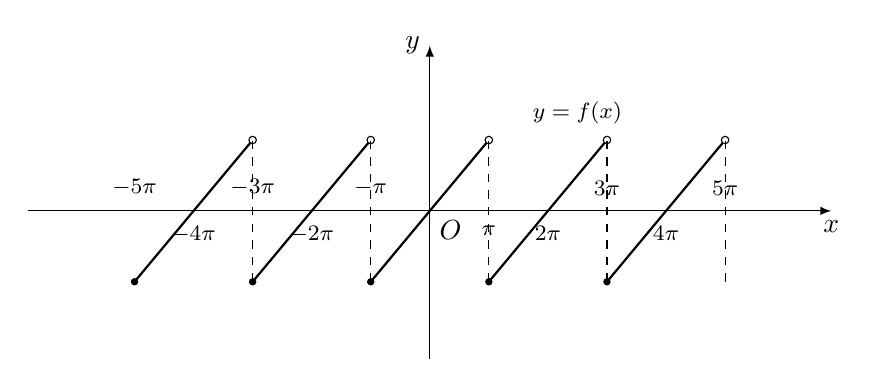
\begin{tikzpicture}[>=latex, scale=0.75]
  \draw[->] (-6.8, 0) -- (6.8, 0) node[below] {$x$};
  \draw[->] (0, -2.5) -- (0, 2.8) node[left] {$y$};
  \node[below right] at (0, 0) {$O$};
  
  \foreach \k in {-2, -1, 0, 1, 2} {
    \draw[thick] (2*\k-1, -1.2) -- (2*\k+1, 1.2);
    \fill (2*\k-1, -1.2) circle (1.8pt);
    \filldraw[fill=white, draw=black] (2*\k+1, 1.2) circle (1.8pt);
    \draw[dashed] (2*\k+1, -1.2) -- (2*\k+1, 1.2);
  }
  
  \draw (-5, 0) node[above=2pt] {\footnotesize $-5\pi$};
  \draw (-4, 0) node[below=2pt] {\footnotesize $-4\pi$};
  \draw (-3, 0) node[above=2pt] {\footnotesize $-3\pi$};
  \draw (-2, 0) node[below=2pt] {\footnotesize $-2\pi$};
  \draw (-1, 0) node[above=2pt] {\footnotesize $-\pi$};
  \draw (1, 0) node[below=2pt] {\footnotesize $\pi$};
  \draw (2, 0) node[below=2pt] {\footnotesize $2\pi$};
  \draw (3, 0) node[above=2pt] {\footnotesize $3\pi$};
  \draw (4, 0) node[below=2pt] {\footnotesize $4\pi$};
  \draw (5, 0) node[above=2pt] {\footnotesize $5\pi$};
  
  \node[above] at (2.5, 1.3) {\footnotesize $y=f(x)$};
\end{tikzpicture}
\caption{}\label{fig:16.1.1}
\end{figure}

\begin{solution}
因为 $x\cos nx$ 与 $x\sin nx$ 分别为奇函数与偶函数, 所以
\[
  a_{n}=\frac{1}{\pi}\int_{-\pi}^{\pi}x\cos nx\,\mathrm{d}x=0,\quad n=0,1,2,\cdots,
\]
\[
  \begin{aligned}
    b_{n}&=\frac{1}{\pi}\int_{-\pi}^{\pi}x\sin nx\,\mathrm{d}x=\frac{2}{\pi}\int_{0}^{\pi}x\sin nx\,\mathrm{d}x=-\frac{2}{n\pi}\int_{0}^{\pi}x\,\mathrm{d}(\cos nx)\\
    &=-\frac{2}{n\pi}\left(\left.x\cos nx\right|_{0}^{\pi}-\int_{0}^{\pi}\cos nx\,\mathrm{d}x\right)=-\frac{2}{n\pi}[\pi(-1)^{n}-0]=(-1)^{n-1}\frac{2}{n},\quad n=1,2,\cdots.
  \end{aligned}
\]
所以,
\[
  f(x)\sim\sum_{n=1}^{\infty}(-1)^{n-1}\frac{2}{n}\sin nx.
\]
根据推论~\ref{cor:16.1.2}, 有
\[
  x=f(x)=\sum_{n=1}^{\infty}(-1)^{n-1}\frac{2}{n}\sin nx,\quad x\in(-\pi,\pi).
\]
进而, 有 (图~\ref{fig:16.1.2})
\[
  \begin{aligned}
    \tilde{f}(x)&=\begin{cases}
      f(x), & x\neq 2k\pi+\pi,\\
      \displaystyle\frac{f(\pi+0)+f(\pi-0)}{2}, & x=2k\pi+\pi,
\end{cases}\quad k=0,\pm 1,\pm 2,\cdots\\
    &=\begin{cases}
      f(x), & x\neq 2k\pi+\pi,\\
      \displaystyle\frac{-\pi+\pi}{2}, & x=2k\pi+\pi,
\end{cases}\quad k=0,\pm 1,\pm 2,\cdots\\
    &=\begin{cases}
      f(x), & x\neq 2k\pi+\pi,\\
      0, & x=2k\pi+\pi,
\end{cases}\quad k=0,\pm 1,\pm 2,\cdots\\
    &=\sum_{n=1}^{\infty}(-1)^{n-1}\frac{2}{n}\sin nx,\quad x\in(-\infty,+\infty).
  \end{aligned}
\]

\begin{figure}[htbp]
\centering
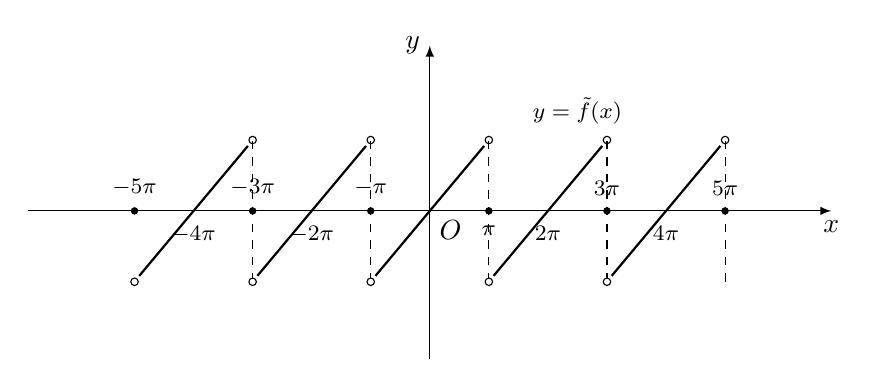
\begin{tikzpicture}[>=latex, scale=0.75]
  \draw[->] (-6.8, 0) -- (6.8, 0) node[below] {$x$};
  \draw[->] (0, -2.5) -- (0, 2.8) node[left] {$y$};
  \node[below right] at (0, 0) {$O$};
  
  \foreach \k in {-2, -1, 0, 1, 2} {
    \draw[thick] (2*\k-0.92, -1.1) -- (2*\k+0.92, 1.1);
    \filldraw[fill=white, draw=black] (2*\k-1, -1.2) circle (1.8pt);
    \filldraw[fill=white, draw=black] (2*\k+1, 1.2) circle (1.8pt);
    \fill (2*\k+1, 0) circle (1.8pt);
    \draw[dashed] (2*\k+1, -1.2) -- (2*\k+1, 1.2);
  }
  \fill (-5, 0) circle (1.8pt);
  
  \draw (-5, 0) node[above=2pt] {\footnotesize $-5\pi$};
  \draw (-4, 0) node[below=2pt] {\footnotesize $-4\pi$};
  \draw (-3, 0) node[above=2pt] {\footnotesize $-3\pi$};
  \draw (-2, 0) node[below=2pt] {\footnotesize $-2\pi$};
  \draw (-1, 0) node[above=2pt] {\footnotesize $-\pi$};
  \draw (1, 0) node[below=2pt] {\footnotesize $\pi$};
  \draw (2, 0) node[below=2pt] {\footnotesize $2\pi$};
  \draw (3, 0) node[above=2pt] {\footnotesize $3\pi$};
  \draw (4, 0) node[below=2pt] {\footnotesize $4\pi$};
  \draw (5, 0) node[above=2pt] {\footnotesize $5\pi$};
  
  \node[above] at (2.5, 1.3) {\footnotesize $y=\tilde{f}(x)$};
\end{tikzpicture}
\caption{}\label{fig:16.1.2}
\end{figure}

取 $x=\displaystyle\frac{\pi}{2}$ 就得到
\[
  \frac{\pi}{2}=\sum_{n=1}^{\infty}(-1)^{n-1}\frac{2}{n}\sin\frac{n\pi}{2},
\]
\[
  \begin{aligned}
    \frac{\pi}{4}&=\sum_{n=1}^{\infty}(-1)^{n-1}\frac{\sin\frac{n\pi}{2}}{n}=\sum_{k=1}^{\infty}(-1)^{2k-2}\frac{\sin\frac{2k-1\pi}{2}}{2k-1}\\
    &=\sum_{k=1}^{\infty}\frac{(-1)^{k-1}}{2k-1}=1-\frac{1}{3}+\frac{1}{5}-\frac{1}{7}+\cdots.
  \end{aligned}
\]
\end{solution}

\begin{example}\label{ex:16.1.2}
设 $f(x)$ 是周期为 $2\pi$ 的函数, 且
\[
  f(x)=\begin{cases}
    x, & x\in(0,2\pi],\\
    2\pi, & x=0.
\end{cases}
\]
求 $f(x)$ 的 Fourier 级数 (图~\ref{fig:16.1.3}) 及函数项级数 $\displaystyle\sum_{n=1}^{\infty}\frac{\sin 2nx}{2n}$, $\displaystyle\sum_{n=1}^{\infty}\frac{\sin 2(n-1)x}{2n-1}$.
\end{example}

\begin{figure}[htbp]
\centering
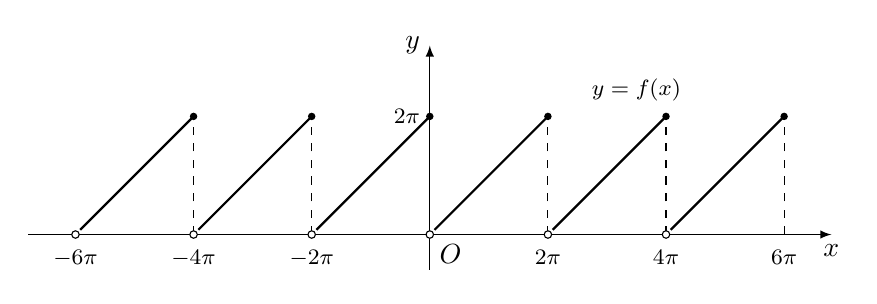
\begin{tikzpicture}[>=latex, scale=0.75]
  \draw[->] (-6.8, 0) -- (6.8, 0) node[below] {$x$};
  \draw[->] (0, -0.6) -- (0, 3.2) node[left] {$y$};
  \node[below right] at (0, 0) {$O$};
  \draw (0, 2) node[left] {\footnotesize $2\pi$};
  
  \foreach \k in {-3, -2, -1, 0, 1, 2} {
    \draw[thick] (2*\k+0.08, 0.08) -- (2*\k+2, 2);
    \filldraw[fill=white, draw=black] (2*\k, 0) circle (1.8pt);
    \fill (2*\k+2, 2) circle (1.8pt);
    \draw[dashed] (2*\k+2, 0) -- (2*\k+2, 2);
  }
  
  \draw (-6, 0) node[below=2pt] {\footnotesize $-6\pi$};
  \draw (-4, 0) node[below=2pt] {\footnotesize $-4\pi$};
  \draw (-2, 0) node[below=2pt] {\footnotesize $-2\pi$};
  \draw (2, 0) node[below=2pt] {\footnotesize $2\pi$};
  \draw (4, 0) node[below=2pt] {\footnotesize $4\pi$};
  \draw (6, 0) node[below=2pt] {\footnotesize $6\pi$};
  
  \node[above] at (3.5, 2.1) {\footnotesize $y=f(x)$};
\end{tikzpicture}
\caption{}\label{fig:16.1.3}
\end{figure}

\begin{solution}
因为
\[
  a_{0}=\frac{1}{\pi}\int_{-\pi}^{\pi}f(x)\,\mathrm{d}x=\frac{1}{\pi}\int_{0}^{2\pi}f(x)\,\mathrm{d}x=\frac{1}{\pi}\int_{0}^{2\pi}x\,\mathrm{d}x=\left.\frac{1}{\pi}\frac{x^{2}}{2}\right|_{0}^{2\pi}=2\pi,
\]
\[
  \begin{aligned}
    a_{n}&=\frac{1}{\pi}\int_{-\pi}^{\pi}f(x)\cos nx\,\mathrm{d}x=\frac{1}{\pi}\int_{0}^{2\pi}f(x)\cos nx\,\mathrm{d}x=\frac{1}{\pi}\int_{0}^{2\pi}x\cos nx\,\mathrm{d}x\\
    &=\frac{1}{n\pi}\int_{0}^{2\pi}x\,\mathrm{d}\sin nx=\frac{1}{n\pi}\left(\left.x\sin nx\right|_{0}^{2\pi}-\int_{0}^{2\pi}\sin nx\,\mathrm{d}x\right)=0,\quad n=1,2,\cdots,
  \end{aligned}
\]
\[
  \begin{aligned}
    b_{n}&=\frac{1}{\pi}\int_{-\pi}^{\pi}f(x)\sin nx\,\mathrm{d}x=\frac{1}{\pi}\int_{0}^{2\pi}f(x)\sin nx\,\mathrm{d}x=\frac{1}{\pi}\int_{0}^{2\pi}x\,\mathrm{d}\left[\frac{\cos nx}{-n}\right]\\
    &=-\frac{1}{n\pi}\left(\left.x\cos nx\right|_{0}^{2\pi}-\int_{0}^{2\pi}\cos nx\,\mathrm{d}x\right)=-\frac{1}{n\pi}(2\pi-0)=-\frac{2}{n},\quad n=1,2,\cdots,
  \end{aligned}
\]
所以,
\[
  f(x)\sim\pi-\sum_{n=1}^{\infty}\frac{2}{n}\sin nx.
\]
根据推论~\ref{cor:16.1.2}, 有
\[
  x=f(x)=\pi-\sum_{n=1}^{\infty}\frac{2}{n}\sin nx,\quad x\in(0,2\pi),
\]
或者
\[
  \frac{\pi-x}{2}=\sum_{n=1}^{\infty}\frac{\sin nx}{n},\quad x\in(0,2\pi).
\]
这正是当年 Abel 给出的例子, 用以说明连续函数项级数的和可能不连续, 根据推论~\ref{cor:13.2.1p}, $\displaystyle\sum_{n=1}^{\infty}\frac{\sin nx}{n}$ 在 $[0,2\pi]$ 上不一致收敛.

进而, 有 (图~\ref{fig:16.1.4})
\[
  \begin{aligned}
    \tilde{f}(x)&=\begin{cases}
      f(x), & x\neq 2k\pi,\\
      \displaystyle\frac{f(0+0)+f(0-0)}{2}, & x=2k\pi,
\end{cases}\quad k=0,\pm 1,\pm 2,\cdots\\
    &=\begin{cases}
      f(x), & x\neq 2k\pi,\\
      \displaystyle\frac{0+2\pi}{2}, & x=2k\pi,
\end{cases}\quad k=0,\pm 1,\pm 2,\cdots\\
    &=\begin{cases}
      f(x), & x\neq 2k\pi,\\
      \pi, & x=2k\pi,
\end{cases}\quad k=0,\pm 1,\pm 2,\cdots\\
    &=\pi-\sum_{n=1}^{\infty}\frac{2}{n}\sin nx,\quad x\in(-\infty,+\infty).
  \end{aligned}
\]

\begin{figure}[htbp]
\centering
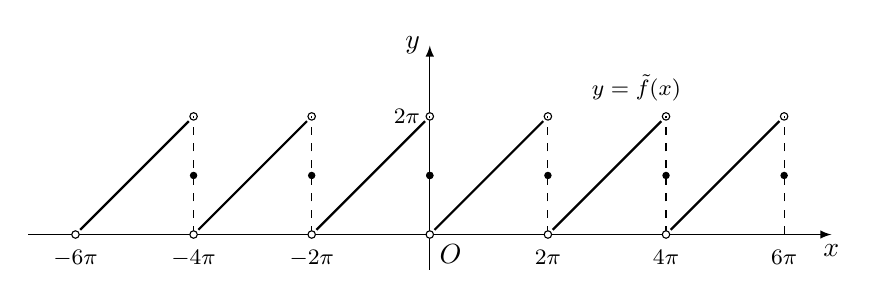
\begin{tikzpicture}[>=latex, scale=0.75]
  \draw[->] (-6.8, 0) -- (6.8, 0) node[below] {$x$};
  \draw[->] (0, -0.6) -- (0, 3.2) node[left] {$y$};
  \node[below right] at (0, 0) {$O$};
  \draw (0, 2) node[left] {\footnotesize $2\pi$};
  
  \foreach \k in {-3, -2, -1, 0, 1, 2} {
    \draw[thick] (2*\k+0.08, 0.08) -- (2*\k+1.92, 1.92);
    \filldraw[fill=white, draw=black] (2*\k, 0) circle (1.8pt);
    \filldraw[fill=white, draw=black] (2*\k+2, 2) circle (1.8pt);
    \fill (2*\k+2, 1) circle (1.8pt);
    \draw[dashed] (2*\k+2, 0) -- (2*\k+2, 2);
  }
  \fill (0, 1) circle (1.8pt);
  
  \draw (-6, 0) node[below=2pt] {\footnotesize $-6\pi$};
  \draw (-4, 0) node[below=2pt] {\footnotesize $-4\pi$};
  \draw (-2, 0) node[below=2pt] {\footnotesize $-2\pi$};
  \draw (2, 0) node[below=2pt] {\footnotesize $2\pi$};
  \draw (4, 0) node[below=2pt] {\footnotesize $4\pi$};
  \draw (6, 0) node[below=2pt] {\footnotesize $6\pi$};
  
  \node[above] at (3.5, 2.1) {\footnotesize $y=\tilde{f}(x)$};
\end{tikzpicture}
\caption{}\label{fig:16.1.4}
\end{figure}

从
\[
  \frac{\pi-x}{2}=\sum_{n=1}^{\infty}\frac{\sin nx}{n},\quad x\in(0,2\pi)
\]
不经计算可得到其他一些有趣的等式. 例如, 将 $x$ 换成 $2x$ 便可得到
\[
  \frac{\pi}{4}-\frac{x}{2}=\sum_{n=1}^{\infty}\frac{\sin 2nx}{2n},\quad x\in(0,\pi).
\]
两式相减就有
\[
  \frac{\pi}{4}=\sum_{n=1}^{\infty}\frac{\sin(2n-1)x}{2n-1},\quad x\in(0,\pi).
\]
令 $x=\displaystyle\frac{\pi}{2}$, 再一次得到
\[
  \frac{\pi}{4}=\sum_{n=1}^{\infty}\frac{\sin(2n-1)\frac{\pi}{2}}{2n-1}=\sum_{n=1}^{\infty}\frac{(-1)^{n-1}}{2n-1}=1-\frac{1}{3}+\frac{1}{5}-\frac{1}{7}+\cdots.
\]
\end{solution}
\begin{example}\label{ex:16.1.3}
将函数 $f(x)=x^{2}$, $x\in[-\pi,\pi]$ 展开为 Fourier 级数. 由此证明:
\[
  \sum_{n=1}^{\infty}\frac{1}{x^{2}}=\frac{\pi^{2}}{6},\quad\sum_{n=1}^{\infty}\frac{(-1)^{n-1}}{n^{2}}=\frac{\pi^{2}}{12}.% 原书如此: 印刷为 x^2, 实为 n^2
\]
\end{example}

\begin{solution}
将 $f(x)$ 的定义延拓到整个数轴上, 使之成为周期为 $2\pi$ 的函数 (图~\ref{fig:16.1.5}), 记延拓后的函数为 $\tilde{f}(x)$, 则 $\tilde{f}(x)$ 是 $(-\infty,+\infty)$ 上的周期为 $2\pi$ 的连续偶函数. 于是,
\[
  a_{0}=\frac{1}{\pi}\int_{-\pi}^{\pi}f(x)\,\mathrm{d}x=\frac{2}{\pi}\int_{0}^{\pi}x^{2}\,\mathrm{d}x=\left.\frac{2}{\pi}\frac{x^{3}}{3}\right|_{0}^{\pi}=\frac{2}{3}\pi^{2},
\]
\[
  \begin{aligned}
    a_{n}&=\frac{1}{\pi}\int_{-\pi}^{\pi}f(x)\cos nx\,\mathrm{d}x=\frac{2}{\pi}\int_{0}^{\pi}x^{2}\cos nx\,\mathrm{d}x=\frac{2}{n\pi}\int_{0}^{\pi}x^{2}\,\mathrm{d}\sin nx\\
    &=\frac{2}{n\pi}\left(\left.x^{2}\sin nx\right|_{0}^{\pi}-\int_{0}^{\pi}2x\sin nx\,\mathrm{d}x\right)=\frac{4}{n^{2}\pi}\int_{0}^{\pi}x\,\mathrm{d}\cos nx\\
    &=\frac{4}{n^{2}\pi}\left(\left.x\cos nx\right|_{0}^{\pi}-\int_{0}^{\pi}cos nx\,\mathrm{d}x\right)=\frac{4}{n^{2}\pi}[\pi(-1)^{n}-0]=(-1)^{n}\frac{4}{n^{2}},\quad n=1,2,\cdots,
  \end{aligned}
\]
\[
  b_{n}=\frac{1}{\pi}\int_{-\pi}^{\pi}f(x)\sin nx\,\mathrm{d}x=\frac{1}{\pi}\int_{-\pi}^{\pi}x^{2}\sin nx\,\mathrm{d}x\xlongequal{\text{奇函数}}0,\quad n=1,2,\cdots.
\]

\begin{figure}[htbp]
\centering
\begin{tikzpicture}[>=latex, scale=0.8]
  \draw[->] (-10.5, 0) -- (10.5, 0) node[below] {$x$};
  \draw[->] (0, -0.6) -- (0, 3.8) node[left] {$y$};
  \node[below right] at (0, 0) {$O$};
  \draw (0, 3.1) node[left] {\footnotesize $\pi^2$};
  
  \foreach \k in {-1, 0, 1} {
    \draw[thick, smooth, domain=-3.14159:3.14159, variable=\t] plot ({2*\k*3.14159/1.8 + \t/1.8}, {(\t)^2 / (3.14159^2) * 3.1});
  }
  
  \draw (-3*3.14159/1.8, 0) node[below=2pt] {\footnotesize $-3\pi$};
  \draw (-2*3.14159/1.8, 0) node[below=2pt] {\footnotesize $-2\pi$};
  \draw (-3.14159/1.8, 0) node[below=2pt] {\footnotesize $-\pi$};
  \draw (3.14159/1.8, 0) node[below=2pt] {\footnotesize $\pi$};
  \draw (2*3.14159/1.8, 0) node[below=2pt] {\footnotesize $2\pi$};
  \draw (3*3.14159/1.8, 0) node[below=2pt] {\footnotesize $3\pi$};
  
  \draw[dashed] (-3*3.14159/1.8, 0) -- (-3*3.14159/1.8, 3.1);
  \draw[dashed] (3*3.14159/1.8, 0) -- (3*3.14159/1.8, 3.1);
  
  \node[above] at (1.8*3.14159/1.8, 3.1) {\footnotesize $y=\tilde{f}(x)$};
\end{tikzpicture}
\caption{}\label{fig:16.1.5}
\end{figure}

根据推论~\ref{cor:16.1.2}, 有
\[
  \tilde{f}(x)=\frac{\pi^{2}}{3}+4\sum_{n=1}^{\infty}\frac{(-1)^{n}}{n^{2}}\cos nx,\quad x\in(-\infty,+\infty).
\]
限制在区间 $[-\pi,\pi]$ 上有
\[
  x^{2}=f(x)=\frac{\pi^{2}}{3}+4\sum_{n=1}^{\infty}\frac{(-1)^{n}}{n^{2}}\cos nx,\quad x\in[-\pi,\pi],
\]
或者
\[
  \sum_{n=1}^{\infty}(-1)^{n}\frac{\cos nx}{n^{2}}=\frac{x^{2}}{4}-\frac{\pi^{2}}{12},\quad x\in[-\pi,\pi].
\]
令 $x=\pi$ 就得
\[
  \sum_{n=1}^{\infty}\frac{1}{n^{2}}=\frac{\pi^{2}}{4}-\frac{\pi^{2}}{12}=\frac{\pi^{2}}{6}.
\]
令 $x=0$ 就得
\[
  \sum_{n=1}^{\infty}\frac{(-1)^{n}}{n^{2}}=\frac{0^{2}}{4}-\frac{\pi^{2}}{12}=-\frac{\pi^{2}}{12},
\]
\[
  \sum_{n=1}^{\infty}\frac{(-1)^{n-1}}{n^{2}}=\frac{\pi^{2}}{12}.
\]
\end{solution}

\begin{example}\label{ex:16.1.4}
设 $a$ 不为整数, 将 $f(x)=\cos ax$ 在 $[-\pi,\pi]$ 上展开为 Fourier 级数并证明
\[
  \frac{\pi}{\sin a\pi}=\frac{1}{a}+\sum_{n=1}^{\infty}(-1)^{n}\frac{2a}{a^{2}-n^{2}},\quad a\notin\mathbb{Z}.
\]
\end{example}

\begin{solution}
将 $f(x)$ 延拓为整个数轴上的以 $2\pi$ 为周期的函数, 记延拓后的函数为 $\tilde{f}(x)$, 则 $\tilde{f}(x)$ 是 $(-\infty,+\infty)$ 上的周期为 $2\pi$ 的连续偶函数. 因此,
\[
  a_{n}=\frac{1}{n}\int_{-\pi}^{\pi}f(x)\cos ax\,\mathrm{d}x=\frac{2}{\pi}\int_{0}^{\pi}\cos ax\cos nx\,\mathrm{d}x% 原书如此: 印刷为 \frac{1}{n} 和 \cos ax
\]
\[
  \begin{aligned}
    &=\frac{1}{\pi}\int_{0}^{\pi}[\cos(a-n)x+\cos(a+n)x]\,\mathrm{d}x=\left.\frac{1}{\pi}\left[\frac{\sin(a-n)x}{a-n}+\frac{\sin(a+n)x}{a+n}\right]\right|_{0}^{\pi}\\
    &=\frac{1}{\pi}\left[\frac{\sin(a-n)\pi}{a-n}+\frac{\sin(a+n)\pi}{a+n}\right]=\frac{1}{\pi}\left[\frac{(-1)^{n}\sin a\pi}{a-n}+\frac{(-1)^{n}\sin a\pi}{a+n}\right]\\
    &=\frac{(-1)^{n}}{\pi}\frac{2a\sin a\pi}{a^{2}-n^{2}},\quad n=0,1,2,\cdots,
  \end{aligned}
\]
\[
  b_{n}=\frac{1}{\pi}\int_{-\pi}^{\pi}f(x)\sin ax\,\mathrm{d}x=\frac{1}{\pi}\int_{-\pi}^{\pi}\cos ax\sin nx\,\mathrm{d}x\xlongequal{\text{奇函数}}0,\quad n=1,2,\cdots.% 原书如此: 前式印刷为 \sin ax
\]
根据推论~\ref{cor:16.1.2}, 可知 $\tilde{f}(x)$ 的 Fourier 级数为
\[
  \tilde{f}(x)=\frac{\sin a\pi}{\pi}\left[\frac{1}{a}+\sum_{n=1}^{\infty}(-1)^{n}\frac{2a}{a^{2}-n^{2}}\cos nx\right],\quad x\in(-\infty,+\infty).
\]
限制在 $[-\pi,\pi]$ 上就有
\[
  \cos ax=\frac{\sin a\pi}{\pi}\left[\frac{1}{a}+\sum_{n=1}^{\infty}(-1)^{n}\frac{2a}{a^{2}-n^{2}}\cos nx\right],\quad x\in[-\pi,\pi].
\]
如果在上式中, 令 $x=0$, 就可得
\[
  \frac{\pi}{\sin a\pi}=\frac{1}{a}+\sum_{n=1}^{\infty}(-1)^{n}\frac{2a}{a^{2}-n^{2}},\quad a\notin\mathbb{Z}.
\]
\end{solution}

应用例~\ref{ex:16.1.4} 中的公式
\[
  \frac{\pi}{\sin a\pi}=\frac{1}{a}+\sum_{n=1}^{\infty}(-1)^{n}\frac{2a}{a^{2}-n^{2}},\quad a\notin\mathbb{Z}
\]
可以计算出下面积分的值.

\begin{example}\label{ex:16.1.5}
证明: 无穷积分
\[
  \int_{0}^{+\infty}\frac{x^{p-1}}{1+x}\,\mathrm{d}x=\frac{1}{p}+\sum_{n=1}^{\infty}(-1)^{n}\frac{2p}{p^{2}-n^{2}}=\frac{\pi}{\sin p\pi},\quad 0<p<1.
\]
\end{example}

\begin{proof}
当 $0<x<1$ 时, 有展开式
\[
  \frac{x^{p-1}}{1+x}=\sum_{n=0}^{\infty}(-1)^{n}x^{n+p-1},
\]
且这个级数在区间 $(0,1)$ 的任何内闭区间 $[a,b]\subset(0,1)$ 上都一致收敛, 如果记它的部分和为 $f_{n}(x)$, 则 $\{f_{n}(x)\}$ 在区间 $(0,1)$ 的任何内闭区间 $[a,b]\subset(0,1)$ 上一致收敛. 由于
\[
  0\leqslant f_{n}(x)=\sum_{k=0}^{n-1}(-1)^{k}x^{k+p-1}=\frac{x^{p-1}[1-(-1)^{n}x^{n}]}{1+x}\leqslant 2\cdot\frac{x^{p-1}}{1+x}\leqslant 2x^{p-1},
\]
而 $\displaystyle\int_{0}^{1}x^{p-1}\,\mathrm{d}x$ 收敛, 故 $\displaystyle\int_{0}^{1}f_{n}(x)\,\mathrm{d}x$ 关于 $n$ 一致收敛.
\[
  \begin{aligned}
    \int_{0}^{1}\frac{x^{p-1}}{1+x}\,\mathrm{d}x&=\int_{0}^{1}\sum_{n=0}^{\infty}(-1)^{n}x^{n+p-1}\,\mathrm{d}x\xlongequal{\text{定理~\ref{thm:15.2.6}}}\sum_{n=0}^{\infty}(-1)^{n}\int_{0}^{1}x^{n+p-1}\,\mathrm{d}x\\
    &=\sum_{n=0}^{\infty}\frac{(-1)^{n}}{n+p}.
  \end{aligned}
\]
进而, 有
\[
  \begin{aligned}
    \int_{1}^{+\infty}\frac{x^{p-1}}{1+x}\,\mathrm{d}x&\xlongequal{x=\frac{1}{t}}\int_{1}^{0}\frac{\left(\frac{1}{t}\right)^{p-1}}{1+\frac{1}{t}}\cdot\frac{-1}{t^{2}}\,\mathrm{d}t=\int_{0}^{1}\frac{t^{-p}}{1+t}\,\mathrm{d}t\\
    &=\int_{0}^{1}\frac{t^{(1-p)+1}}{1+t}\,\mathrm{d}t\xlongequal{\text{由上面结果}}\sum_{n=0}^{\infty}\frac{(-1)^{n}}{n+1-p}=\sum_{n=1}^{\infty}\frac{(-1)^{n}}{p-n}.% 原书如此: 印刷为 t^{(1-p)+1}
  \end{aligned}
\]
综合上述得到
\[
  \begin{aligned}
    \int_{0}^{+\infty}\frac{x^{p-1}}{1+x}\,\mathrm{d}x&=\int_{0}^{1}\frac{x^{p-1}}{1+x}\,\mathrm{d}x+\int_{1}^{+\infty}\frac{x^{p-1}}{1+x}\,\mathrm{d}x\\
    &=\sum_{n=0}^{\infty}\frac{(-1)^{n}}{p+n}+\sum_{n=1}^{\infty}\frac{(-1)^{n}}{p-n}=\frac{1}{p}+\sum_{n=1}^{\infty}(-1)^{n}\frac{2p}{p^{2}-n^{2}}\\
    &\xlongequal{\text{例~\ref{ex:16.1.4}}}\frac{\pi}{\sin p\pi},\quad 0<p<1.
  \end{aligned}
\]
\end{proof}

\begin{example}\label{ex:16.1.6}
将函数 $\mathrm{e}^{ax}$ 在区间 $(0,2\pi)$ 上展开为 Fourier 级数, 并求 $\displaystyle\sum_{n=1}^{\infty}\frac{1}{1+n^{2}}$.
\end{example}

\begin{solution}
先计算 Fourier 系数:
\[
  \begin{aligned}
    a_{n}&=\frac{1}{\pi}\int_{0}^{2\pi}\mathrm{e}^{ax}\cos nx\,\mathrm{d}x=\left.\frac{1}{\pi}\frac{\mathrm{e}^{ax}}{a^{2}+n^{2}}(a\cos nx+n\sin nx)\right|_{0}^{2\pi}\\
    &=\frac{\mathrm{e}^{2\pi a}-1}{\pi}\frac{a}{a^{2}+n^{2}},\quad n=0,1,2,\cdots.
  \end{aligned}
\]
\[
  \begin{aligned}
    b_{n}&=\frac{1}{\pi}\int_{0}^{2\pi}\mathrm{e}^{ax}\sin nx\,\mathrm{d}x=\left.\frac{1}{\pi}\frac{\mathrm{e}^{ax}}{a^{2}+n^{2}}(a\sin nx-n\cos nx)\right|_{0}^{2\pi}\\
    &=\frac{\mathrm{e}^{2\pi a}-1}{\pi}\frac{-n}{a^{2}+n^{2}},\quad n=1,2,\cdots.
  \end{aligned}
\]
于是,
\[
  \mathrm{e}^{ax}=\frac{\mathrm{e}^{2\pi a}-1}{\pi}\left(\frac{1}{2a}+\sum_{n=1}^{\infty}\frac{a\cos nx-n\sin nx}{a^{2}+n^{2}}\right),\quad 0<x<2\pi.
\]
如果将 $f(x)=\mathrm{e}^{ax}$ ($0<x<2\pi$) 延拓为 $(-\infty,+\infty)$ 上以 $2\pi$ 为周期的函数 $\tilde{f}(x)$, 则必须有
\[
  \tilde{f}(0)=\tilde{f}(2\pi)=\frac{f(2\pi-0)+f(0+0)}{2}=\frac{\mathrm{e}^{2\pi a}+\mathrm{e}^{0\cdot a}}{2}=\frac{\mathrm{e}^{2\pi a}+1}{2}.
\]
由此得到
\[
  \tilde{f}(x)=\frac{\mathrm{e}^{2\pi a}-1}{\pi}\left(\frac{1}{2a}+\sum_{n=1}^{\infty}\frac{a\cos nx-n\sin nx}{a^{2}+n^{2}}\right),\quad -\infty<x<+\infty.
\]
令 $a=1$, $x=0$, 就有
\[
  \frac{\mathrm{e}^{2\pi}+1}{2}=\frac{\mathrm{e}^{2\pi}-1}{\pi}\left(\frac{1}{2}+\sum_{n=1}^{\infty}\frac{1}{1+n^{2}}\right),
\]
即
\[
  \sum_{n=1}^{\infty}\frac{1}{1+n^{2}}=\frac{\mathrm{e}^{2\pi}+1}{2}\cdot\frac{\pi}{\mathrm{e}^{2\pi}-1}-\frac{1}{2}=\frac{\pi}{2}\frac{\mathrm{e}^{2\pi}+1}{\mathrm{e}^{2\pi}-1}-\frac{1}{2}.
\]
\end{solution}

\begin{remark}\label{rem:16.1.2}
从例~\ref{ex:16.1.1}$\sim$例~\ref{ex:16.1.4}, 例~\ref{ex:16.1.6} 可看到, 经某个函数的 Fourier 级数的计算, 并取特殊点求得一些数项级数之和, 这些数项级数之和是难以用其他方法得到的.
\end{remark}

上面各例都是先给出函数在 $(-\pi,\pi)$ 或 $(0,2\pi)$ 上的表达式, 然后将它延拓为整个数轴上的周期 $2\pi$ 的函数, 再将它展开为 Fourier 级数.

对于只在 $(0,\pi)$ 上定义的函数, 如何展开为 Fourier 级数呢? 这时, 在 $(-\pi,0)$ 上可以任意补充 $f(x)$ 的定义, 使 $f(x)$ 在 $(-\pi,\pi)$ 上有定义, 然后再将它以 $2\pi$ 为周期延拓到整个数轴上去. 对于各种不同的延拓, 得到的 Fourier 级数自然也是不同的. 但在 $(0,\pi)$ 上, 它们都收敛到同一个函数. 而偶性延拓与奇性延拓是常用的两种延拓方法.

\begin{definition}\label{def:16.1.3}
设 $f(x)$ 是定义在 $(0,\pi)$ 上的函数, 令
\[
  f(x)=f(-x),\quad x\in(-\pi,0)
\]
来补充 $f(x)$ 在 $(-\pi,0)$ 上的定义, 使 $f(x)$ 在 $(-\pi,\pi)$ 上成为偶函数 (延拓后的函数 $\tilde{f}(x)$ 仍记为 $f(x)$), 这种延拓方法称为\textbf{偶性延拓}. 这样便有
\[
  a_{n}=\frac{1}{\pi}\int_{-\pi}^{\pi}f(x)\cos nx\,\mathrm{d}x=\frac{2}{\pi}\int_{0}^{\pi}f(x)\cos nx\,\mathrm{d}x,\quad n=0,1,2,\cdots,
\]
\[
  b_{n}=\frac{1}{\pi}\int_{-\pi}^{\pi}f(x)\sin nx\,\mathrm{d}x=0,\quad n=1,2,\cdots.
\]
因此, $f(x)$ 的 Fourier 级数中只含余弦项:
\[
  f(x)\sim\frac{a_{0}}{2}+\sum_{n=1}^{\infty}a_{n}\cos nx,
\]
称它为 $f(x)$, $x\in(0,\pi)$ 的\textbf{余弦级数}.

如果令
\[
  f(x)=-f(-x),\quad x\in(-\pi,0)
\]
来补充 $f(x)$ 在 $(-\pi,0)$ 上的定义, 使 $f(x)$ 在 $(-\pi,\pi)$ 上成为奇函数 (延拓后的函数 $\tilde{f}(x)$ 仍记为 $f(x)$), 这种延拓方法称为\textbf{奇性延拓} (注意: 由 $f(0)=f(-0)=-f(0)$, 知 $f(0)=0$). 这样便有
\[
  a_{n}=\frac{1}{\pi}\int_{-\pi}^{\pi}f(x)\cos nx\,\mathrm{d}x=0,\quad n=0,1,2,\cdots,
\]
\[
  b_{n}=\frac{1}{\pi}\int_{-\pi}^{\pi}f(x)\sin nx\,\mathrm{d}x=\frac{2}{\pi}\int_{0}^{\pi}f(x)\sin nx\,\mathrm{d}x,\quad n=1,2,\cdots.
\]
因此, $f(x)$ 的 Fourier 级数中只含正弦项:
\[
  f(x)\sim\sum_{n=1}^{\infty}b_{n}\sin nx,
\]
称它为 $f(x)$, $x\in(0,\pi)$ 的\textbf{正弦级数}.
\end{definition}

由此可见, 对于只定义在区间 $(0,\pi)$ 上的函数, 只要满足 Dini 定理的条件, 就可考虑它的正弦级数, 也可考虑它的余弦级数.

\begin{example}\label{ex:16.1.7}
将函数
\[
  f(x)=x,\quad x\in(0,\pi)
\]
分别展开为余弦级数与正弦级数.
\end{example}

\begin{solution}
若要展开成余弦级数, 可先将 $f(x)$, $x\in(0,\pi)$ 偶性延拓到区间 $(-\pi,0)$ 上, 然后再将它以周期 $2\pi$ 延拓到整个区间 $(-\infty,+\infty)$ 上, 所得的函数记为 $\tilde{f}(x)$ (图~\ref{fig:16.1.6}). 于是,
\[
  a_{0}=\frac{2}{\pi}\int_{0}^{\pi}x\,\mathrm{d}x=\pi,
\]
\[
  \begin{aligned}
    a_{n}&=\frac{2}{\pi}\int_{0}^{\pi}x\cos nx\,\mathrm{d}x=\frac{2}{n\pi}\int_{0}^{\pi}x\,\mathrm{d}\sin nx\\
    &=\frac{2}{n\pi}\left(\left.x\sin nx\right|_{0}^{\pi}-\int_{0}^{\pi}\sin nx\,\mathrm{d}x\right)=\left.\frac{2}{n^{2}\pi}\cos nx\right|_{0}^{\pi}\\
    &=\frac{2}{n^{2}\pi}[(-1)^{n}-1]=\begin{cases}
      0, & n=2k,\\
      \displaystyle-\frac{4}{(2k-1)^{2}\pi}, & n=2k-1,
\end{cases}\quad k=1,2,\cdots,
  \end{aligned}
\]
\[
  b_{n}=0,\quad n=1,2,\cdots.
\]
所以,
\[
  x=\frac{\pi}{2}-\frac{4}{\pi}\sum_{k=1}^{\infty}\frac{\cos(2k-1)x}{(2k-1)^{2}},\quad x\in[0,\pi].% 原书如此: 公式中分子印刷为 \cos(2k-1)\pi
\]
\[
  \tilde{f}(x)=\frac{\pi}{2}-\frac{4}{\pi}\sum_{k=1}^{\infty}\frac{\cos(2k-1)x}{(2k-1)^{2}},\quad x\in(-\infty,+\infty).% 原书如此: 同样印刷为 \cos(2k-1)\pi
\]

\begin{figure}[htbp]
\centering
\begin{tikzpicture}[>=latex, scale=0.85]
  \draw[->] (-7.5, 0) -- (7.5, 0) node[below] {$x$};
  \draw[->] (0, -0.6) -- (0, 3.2) node[left] {$y$};
  \node[below right] at (0, 0) {$O$};
  
  % 刻度标记
  \draw (-2*2.2, 0) node[below=2pt] {\footnotesize $-2\pi$};
  \draw (-2.2, 0) node[below=2pt] {\footnotesize $-\pi$};
  \draw (2.2, 0) node[below=2pt] {\footnotesize $\pi$};
  \draw (2*2.2, 0) node[below=2pt] {\footnotesize $2\pi$};
  
  % 折线段
  \draw[thick] (-2*2.2, 0) -- (-2.2, 2.2);
  \draw[thick, dashed] (-2.2, 2.2) -- (0, 0);
  \draw[thick] (0, 0) -- (2.2, 2.2) -- (2*2.2, 0);
  \draw[thick] (-2*2.2, 0) -- (-2.6*2.2, 0.6*2.2);
  \draw[thick] (2*2.2, 0) -- (2.6*2.2, 0.6*2.2);
\end{tikzpicture}
\caption{}\label{fig:16.1.6}
\end{figure}

令 $x=0$ 得
\[
  \sum_{k=1}^{\infty}\frac{1}{(2k-1)^{2}}=\frac{\pi^{2}}{8}.
\]
此数项级数之和也可如下得到:
\[
  \sum_{n=1}^{\infty}\frac{1}{n^{2}}=\sum_{k=1}^{\infty}\frac{1}{(2k-1)^{2}}+\sum_{k=1}^{\infty}\frac{1}{(2k)^{2}},
\]
\[
  \sum_{k=1}^{\infty}\frac{1}{(2k-1)^{2}}=\sum_{n=1}^{\infty}\frac{1}{n^{2}}-\sum_{k=1}^{\infty}\frac{1}{(2k)^{2}}=\frac{3}{4}\sum_{n=1}^{\infty}\frac{1}{n^{2}}\xlongequal{\text{例~\ref{ex:16.1.3}}}\frac{3}{4}\times\frac{\pi^{2}}{6}=\frac{\pi^{2}}{8}.
\]
若要展开成正弦级数, 可先将 $f(x)$, $x\in(0,\pi)$ 奇性延拓到 $(-\pi,0)$ 上, 然后再将它以周期 $2\pi$ 延拓到整个区间 $(-\infty,+\infty)$ 上, 所得的函数记为 $\tilde{f}(x)$ (图~\ref{fig:16.1.7}). 于是, 由例~\ref{ex:16.1.1} 知
\[
  x=2\sum_{n=1}^{\infty}(-1)^{n-1}\frac{\sin nx}{n},\quad x\in[0,\pi).
\]

\begin{figure}[htbp]
\centering
\begin{tikzpicture}[>=latex, scale=0.85]
  \draw[->] (-8.5, 0) -- (8.5, 0) node[below] {$x$};
  \draw[->] (0, -2.6) -- (0, 2.8) node[left] {$y$};
  \node[below right] at (0, 0) {$O$};
  
  % 刻度标记
  \draw (-3*2.2, 0) node[below=2pt] {\footnotesize $-3\pi$};
  \draw (-2*2.2, 0) node[below=2pt] {\footnotesize $-2\pi$};
  \draw (-2.2, 0) node[below=2pt] {\footnotesize $-\pi$};
  \draw (2.2, 0) node[below=2pt] {\footnotesize $\pi$};
  \draw (2*2.2, 0) node[below=2pt] {\footnotesize $2\pi$};
  \draw (3*2.2, 0) node[below=2pt] {\footnotesize $3\pi$};
  
  % 中间周期
  \draw[thick, dashed] (-2.2+0.05, -1.8+0.05) -- (0, 0);
  \draw[thick] (0, 0) -- (2.2-0.05, 1.8-0.05);
  \filldraw[fill=white, draw=black] (-2.2, -1.8) circle (1.8pt);
  \filldraw[fill=white, draw=black] (2.2, 1.8) circle (1.8pt);
  
  % 右侧周期
  \draw[thick] (2.2+0.05, -1.8+0.05) -- (3*2.2-0.05, 1.8-0.05);
  \filldraw[fill=white, draw=black] (2.2, -1.8) circle (1.8pt);
  \filldraw[fill=white, draw=black] (3*2.2, 1.8) circle (1.8pt);
  
  % 左侧周期
  \draw[thick] (-3*2.2+0.05, -1.8+0.05) -- (-2.2-0.05, 1.8-0.05);
  \filldraw[fill=white, draw=black] (-3*2.2, -1.8) circle (1.8pt);
  \filldraw[fill=white, draw=black] (-2.2, 1.8) circle (1.8pt);
\end{tikzpicture}
\caption{}\label{fig:16.1.7}
\end{figure}

如果 $\tilde{f}[(2k-1)\pi]=\frac{\pi+(-\pi)}{2}=0$, 则
\[
  \tilde{f}(x)=2\sum_{n=1}^{\infty}(-1)^{n-1}\frac{\sin nx}{n},\quad x\in(-\infty,+\infty).
\]
\end{solution}

下面来讨论周期为 $2l$ 的函数的 Fourier 展开.

\begin{definition}\label{def:16.1.4}
设 $f(x)$ 是以 $2l$ 为周期的函数, 作变换 $x=\frac{l}{\pi}t$, 并记
\[
  f(x)=f\left(\frac{l}{\pi}t\right)=g(t),
\]
则 $g(t)$ 是周期为 $2\pi$ 的函数. 如果 $g(t)$ 满足 Dini 定理推论的条件, 便有
\[
  g(t)=\frac{a_{0}}{2}+\sum_{n=1}^{\infty}(a_{n}\cos nt+b_{n}\sin nt),\quad t\in(-\infty,+\infty),
\]
其中
\[
  a_{n}=\frac{1}{\pi}\int_{-\pi}^{\pi}g(t)\cos nt\,\mathrm{d}t,\quad n=0,1,2,\cdots,
\]
\[
  b_{n}=\frac{1}{\pi}\int_{-\pi}^{\pi}g(t)\sin nt\,\mathrm{d}t,\quad n=1,2,\cdots.
\]
回到原来的变量 $x$ 就有
\[
  f(x)=\frac{a_{0}}{2}+\sum_{n=1}^{\infty}\left(a_{n}\cos\frac{n\pi}{l}x+b_{n}\sin\frac{n\pi}{l}x\right),\quad x\in(-\infty,+\infty),
\]
而
\[
  \begin{aligned}
    a_{n}&=\frac{1}{\pi}\int_{-\pi}^{\pi}g(t)\cos nt\,\mathrm{d}t\xlongequal{t=\frac{\pi}{l}x}\frac{1}{\pi}\int_{-l}^{l}f(x)\cos\frac{n\pi}{l}x\,\mathrm{d}\left(\frac{\pi}{l}x\right)\\
    &=\frac{1}{l}\int_{-l}^{l}f(x)\cos\frac{n\pi}{l}x\,\mathrm{d}x,\quad n=0,1,2,\cdots,
  \end{aligned}
\]
\[
  \begin{aligned}
    b_{n}&=\frac{1}{\pi}\int_{-\pi}^{\pi}g(t)\sin nt\,\mathrm{d}t\xlongequal{t=\frac{\pi}{l}x}\frac{1}{\pi}\int_{-l}^{l}f(x)\sin\frac{n\pi}{l}x\,\mathrm{d}\left(\frac{\pi}{l}x\right)\\
    &= \frac{1}{l}\int_{-l}^{l}f(x)\sin\frac{n\pi}{l}x\,\mathrm{d}x,\quad n=1,2,\cdots.
  \end{aligned}
\]
这就给出了周期 $2l$ 的函数 $f(x)$ 的 Fourier 展开式.

如果 $f(x)$ 只定义在 $(0,l)$ 上, 则它既可展开为余弦级数
\[
  f(x)=\frac{a_{0}}{2}+\sum_{n=1}^{\infty}a_{n}\cos\frac{n\pi}{l}x,
\]
其中
\[
  a_{n}=\frac{2}{l}\int_{0}^{l}f(x)\cos\frac{n\pi}{l}x\,\mathrm{d}x,\quad n=0,1,2,\cdots,
\]
也可展开为正弦级数
\[
  f(x)=\sum_{n=1}^{\infty}b_{n}\sin\frac{n\pi}{l}x,
\]
其中
\[
  b_{n}=\frac{2}{l}\int_{0}^{l}f(x)\sin\frac{n\pi}{l}x\,\mathrm{d}x,\quad n=1,2,\cdots.
\]
\end{definition}

\begin{example}\label{ex:16.1.8}
将函数
\[
  f(x)=\begin{cases}
    x, & x\in\left[0,\dfrac{l}{2}\right],\\
    l-x, & x\in\left[\dfrac{l}{2},l\right]
\end{cases}
\]
在 $[0,l]$ 上展开为正弦级数.
\end{example}

\begin{solution}
将 $f(x)$ 作奇性延拓 (图~\ref{fig:16.1.8}) 得 $\tilde{f}(x)$, 则
\[
  \begin{aligned}
    b_{n}&=\frac{2}{l}\int_{0}^{l}f(x)\sin\frac{n\pi}{l}x\,\mathrm{d}x\\
    &=\frac{2}{l}\int_{0}^{\frac{l}{2}}x\sin\frac{n\pi}{l}x\,\mathrm{d}x+\frac{2}{l}\int_{\frac{l}{2}}^{l}(l-x)\sin\frac{n\pi}{l}x\,\mathrm{d}x\\
    &=\frac{2}{l}\int_{0}^{\frac{l}{2}}x\,\mathrm{d}\left(-\frac{l}{n\pi}\cos\frac{n\pi}{l}x\right)+\frac{2}{l}\int_{\frac{l}{2}}^{l}(l-x)\,\mathrm{d}\left(-\frac{l}{n\pi}\cos\frac{n\pi}{l}x\right)\\
    &=\frac{2}{l}\left(-\left.\frac{l}{n\pi}x\cos\frac{n\pi}{l}x\right|_{0}^{\frac{l}{2}}+\int_{0}^{\frac{l}{2}}\frac{l}{n\pi}\cos\frac{n\pi}{l}x\,\mathrm{d}x\right.\\
    &\quad\left.-\left.\frac{l}{n\pi}(l-x)\cos\frac{n\pi}{l}x\right|_{\frac{l}{2}}^{l}-\frac{l}{n\pi}\int_{\frac{l}{2}}^{l}\cos\frac{n\pi}{l}x\,\mathrm{d}x\right)\\
    &=\frac{2}{n\pi}\left(-\frac{l}{2}\cos\frac{n\pi}{2}+\left.\frac{l}{n\pi}\sin\frac{n\pi}{l}x\right|_{0}^{\frac{l}{2}}+\frac{l}{2}\cos\frac{n\pi}{2}-\left.\frac{l}{n\pi}\sin\frac{n\pi}{l}x\right|_{\frac{l}{2}}^{l}\right)\\
    &=\frac{2}{n\pi}\left(\frac{l}{n\pi}\sin\frac{n\pi}{2}+\frac{l}{n\pi}\sin\frac{n\pi}{2}\right)=\frac{4l}{n^{2}\pi^{2}}\sin\frac{n\pi}{2}\\
    &=\begin{cases}
      0, & n=2k,\\
      \displaystyle\frac{4l}{\pi^{2}}\frac{(-1)^{k}}{(2k+1)^{2}}, & n=2k+1,
\end{cases}\quad k=0,1,2,\cdots.
  \end{aligned}
\]
由此得到 $f(x)$, $x\in[0,l]$ 的正弦展开式为
\[
  f(x)=\frac{4l}{\pi^{2}}\sum_{k=0}^{\infty}\frac{(-1)^{k}}{(2k+1)^{2}}\sin\frac{2k+1}{l}\pi x,\quad x\in[0,l].% 原书如此: 印刷为 x\in[0,1]
\]
\[
  \tilde{f}(x)=\frac{4l}{\pi^{2}}\sum_{k=0}^{\infty}\frac{(-1)^{k}}{(2k+1)^{2}}\sin\frac{2k+1}{l}\pi x,\quad x\in(-\infty,+\infty).
\]
\end{solution}

\begin{center}
\begin{minipage}{\linewidth}
\centering
\begin{tikzpicture}[>=latex, scale=0.75]
  \draw[->] (-5, 0) -- (5, 0) node[below] {$x$};
  \draw[->] (0, -2.2) -- (0, 2.4) node[left] {$y$};
  \node[below right] at (0, 0) {$O$};
  
  \coordinate (L2) at (1.6, 0);
  \coordinate (L) at (3.2, 0);
  \coordinate (NL2) at (-1.6, 0);
  \coordinate (NL) at (-3.2, 0);
  \coordinate (TOP) at (1.6, 1.6);
  \coordinate (BOT) at (-1.6, -1.6);
  
  % 实线部分 (正侧)
  \draw[thick] (0, 0) -- (TOP) -- (L);
  % 虚线部分 (负侧奇延拓)
  \draw[thick, dashed] (NL) -- (BOT) -- (0, 0);
  
  % 辅助线
  \draw[dashed] (0, 1.6) node[left] {\footnotesize $\dfrac{l}{2}$} -- (TOP) -- (1.6, 0);
  \draw[dashed] (0, -1.6) node[right=1pt] {\footnotesize $-\dfrac{l}{2}$} -- (BOT) -- (-1.6, 0);
  
  % 坐标标注
  \draw (1.6, 0) node[below=2pt] {\footnotesize $\dfrac{l}{2}$};
  \draw (3.2, 0) node[below=2pt] {\footnotesize $l$};
  \draw (-1.6, 0) node[above=2pt] {\footnotesize $-\dfrac{l}{2}$};
  \draw (-3.2, 0) node[below=2pt] {\footnotesize $-l$};
  
  \node[above] at (1.5, 0.9) {\footnotesize $f(x)$};
\end{tikzpicture}
\captionof{figure}{}\label{fig:16.1.8}
\end{minipage}
\end{center}

\begin{exblock}{练习题 16.1}
\item 证明: 三角多项式
\[
  T_{n}(x)=\sum_{k=0}^{n}(\alpha_{k}\cos kx+\beta_{k}\sin kx)
\]
的 Fourier 级数就是它本身.
\item 设 $f(x)$ 是周期为 $2\pi$ 的可积或绝对可积函数. 证明:

(1) 如果 $f(x)$ 在 $[-\pi,\pi]$ 中满足 $f(x+\pi)=f(x)$, 则 $a_{2n-1}=b_{2n-1}=0$, $n=1,2,\cdots$;

(2) 如果 $f(x)$ 在 $[-\pi,\pi]$ 中满足 $f(x+\pi)=-f(x)$, 则 $a_{2n}=b_{2n}=0$, $n=0,1,2,\cdots$.
\item 设 $a_{n}, b_{n}$ 是周期为 $2\pi$ 的可积或绝对可积函数 $f(x)$ 的 Fourier 系数. 证明: 平移函数 $f(x+h)$ 的 Fourier 系数为
\[
  \tilde{a}_{n}=a_{n}\cos nh+b_{n}\sin nh,\quad n=0,1,2,\cdots,% 原书如此: 印刷为 \cosh 和 \sinh
\]
\[
  \tilde{b}_{n}=b_{n}\cos nh-a_{n}\sin nh,\quad n=1,2,\cdots.
\]
\item 如果级数
\[
  \frac{|a_{0}|}{2}+\sum_{k=1}^{\infty}(|a_{k}|+|b_{k}|)<+\infty,
\]
则级数
\[
  \frac{a_{0}}{2}+\sum_{k=1}^{\infty}(a_{k}\cos kx+b_{k}\sin kx)
\]
必是某个周期为 $2\pi$ 的函数的 Fourier 级数.
\item 计算极限 $\displaystyle\lim_{\lambda\to\infty}\int_{0}^{1}\ln x\cos^{2}\lambda x\,\mathrm{d}x$.
\item 将函数
\[
  f(x)=\operatorname{sgn}x,\quad x\in(-\pi,\pi)
\]
展开为 Fourier 级数, 并利用这个级数求级数 $\displaystyle\sum_{n=1}^{\infty}\frac{(-1)^{n-1}}{2n-1}$ 的和.
\item 在区间 $(-\pi,\pi)$ 上将下列函数展开为 Fourier 级数:

(1) $|x|$; \qquad (2) $\sin ax$; \qquad (3) $x\sin x$.
\item 将 $f(x)=x-[x]$ 在 $[0,1]$ 上展开为 Fourier 级数.
\item 在区间 $(-l,l)$ 上将下列函数展开为 Fourier 级数:

(1) $x$; \qquad (2) $x+|x|$.
\item 将函数
\[
  f(x)=\begin{cases}
    x, & 0\leqslant x\leqslant 1,\\
    1, & 1<x<2,\\
    3-x, & 2\leqslant x\leqslant 3
\end{cases}
\]
展开为 Fourier 级数.
\end{exblock}

\begin{exblock}{思考题 16.1}
\item 设 $f(x)$ 是周期为 $2\pi$ 的可积或绝对可积函数, $b_{n}$ ($n=1,2,\cdots$) 是其 Fourier 系数. 证明:

(1) 如果 $f(x)$ 在 $(0,2\pi)$ 中单调减少, 则 $b_{n}\geqslant 0$;

(2) 如果 $f(x)$ 在 $(0,2\pi)$ 中单调增加, 则 $b_{n}\leqslant 0$.
\item 设 $f(x)$ 是周期为 $2\pi$ 的 Riemann 可积函数, 如果它在 $(-\pi,\pi)$ 中单调, 证明:
\[
  a_{n}=O\left(\frac{1}{n}\right),\quad b_{n}=O\left(\frac{1}{n}\right),\quad n\to+\infty.
\]
\item 设 $f(x)$ 在 $[a,b]$ 上 Riemann 可积, 证明:
\[
  \lim_{n\to+\infty}\int_{a}^{b}f(x)|\sin nx|\,\mathrm{d}x=\frac{2}{\pi}\int_{a}^{b}f(x)\,\mathrm{d}x;
\]
\[
  \lim_{n\to+\infty}\int_{a}^{b}f(x)|\cos nx|\,\mathrm{d}x=\frac{2}{\pi}\int_{a}^{b}f(x)\,\mathrm{d}x.
\]
\item 设 $f(x)$ 在 $(-\infty,+\infty)$ 上绝对可积, 证明:
\[
  \lim_{n\to+\infty}\int_{-\infty}^{+\infty}f(x)|\sin nx|\,\mathrm{d}x=\frac{2}{\pi}\int_{-\infty}^{+\infty}f(x)\,\mathrm{d}x;
\]
\[
  \lim_{n\to+\infty}\int_{-\infty}^{+\infty}f(x)|\cos nx|\,\mathrm{d}x=\frac{2}{\pi}\int_{-\infty}^{+\infty}f(x)\,\mathrm{d}x.% 原书如此: 印刷为 f(x)f(x)
\]
\item 证明: 对任意 $x\in(-\infty,+\infty)$ 有
\[
  |\cos x|=\frac{2}{\pi}+\frac{4}{\pi}\sum_{n=1}^{\infty}\frac{(-1)^{n+1}}{4n^{2}-1}\cos 2nx.
\]
由此结果证明: 如果 $f(x)$ 在 $[a,b]$ 中 Riemann 可积, 则
\[
  \lim_{\lambda\to+\infty}\int_{a}^{b}f(x)|\cos\lambda x|\,\mathrm{d}x=\frac{2}{\pi}\int_{a}^{b}f(x)\,\mathrm{d}x
\]
(参阅题 3).
\item 将函数 $f(x)=\ln\left(2\cos\dfrac{x}{2}\right)$ 在 $(-\pi,\pi)$ 上展开为 Fourier 级数, 由此证明:
\[
  \sum_{n=1}^{\infty}\frac{\cos nx}{n}=-\ln\left(2\sin\frac{x}{2}\right),\quad 0<x<2\pi.
\]
\item 设函数
\[
  \varphi(-x)=\psi(x),
\]
问: $\varphi(x)$ 与 $\psi(x)$ 的 Fourier 系数 $a_{n}, b_{n}$ 与 $\alpha_{n}, \beta_{n}$ 之间有何关系?
\item 设函数 $\varphi(-x)=-\psi(x)$, 问 $\varphi(x)$ 与 $\psi(x)$ 的 Fourier 系数 $a_{n}, b_{n}$ 与 $\alpha_{n}, \beta_{n}$ 之间有何关系?
\item 已知周期为 $2\pi$ 的可积函数 $f(x)$ 的 Fourier 系数为 $a_{n}, b_{n}$. 试计算函数
\[
  f_{h}(x)=\frac{1}{2h}\int_{x-h}^{x+h}f(\xi)\,\mathrm{d}\xi
\]
的 Fourier 系数 $A_{n}, B_{n}$.
\item 设 $f(x)$ 是以 $2\pi$ 为周期的连续函数, 并且 $a_{n}, b_{n}$ 为其 Fourier 系数. 求卷积函数
\[
  F(x)=\frac{1}{\pi}\int_{-\pi}^{\pi}f(t)f(x+t)\,\mathrm{d}t
\]
的 Fourier 系数 $A_{n}, B_{n}$.
\end{exblock}

% ====================================================================
%  徐森林、金亚东、薛春华《数学分析》（第三册）
%  \S16.2  平方平均收敛
%  源：原书印刷页 267–286（PDF 物理页 273–292）
%  约定：全西文标点；行间公式用一对方括号；多行公式用 align 或 aligned；
%        跨册引用一律用 extref；数学模式内的中文必须包 text
% ====================================================================
\section{平方平均收敛}\label{sec:16.2}

定理~\ref{thm:14.3.8} 中已经证明, 周期为 $2\pi$ 的连续函数能用三角多项式一致逼近. 根据定理~\ref{thm:13.2.1} 知, 能用周期为 $2\pi$ 的三角多项式一致逼近的函数必是周期为 $2\pi$ 的连续函数. 因此, 周期为 $2\pi$ 的且在 $[-\pi, \pi]$ 上可积的函数, 只要它不连续(如: $f(x) = \begin{cases} 0, & x \neq 2k\pi, \\ 1, & x = 2k\pi, \end{cases}\ k = 0, \pm 1, \pm 2, \cdots$) 就不能用三角多项式一致逼近. 问题出在哪里呢? 所谓一致逼近, 就是
\[
  \sup_{-\pi\leqslant x\leqslant\pi}\left|f(x)-T_{n}(x)\right|\to0,\quad n\to+\infty.
\]
这就要求 $f(x)$ 与三角多项式 $T_{n}(x)$ 之差在整个 $[-\pi, \pi]$ 上均匀地趋于 $0$, 而不允许有点例外. 由于连续函数在邻近点处的值相差很小, 上述要求能办到, 而一般的周期为 $2\pi$ 的且在 $[-\pi, \pi]$ 上可积的函数就不一定做得到了. 在这种情况下, 我们只能放弃一致逼近, 退而求其次, 要求能用三角多项式 $T_{n}(x)$ 平均地逼近 $f(x)$, 即
\[
  \int_{-\pi}^{\pi}\left[f(x)-T_{n}(x)\right]^{2}\mathrm{d}x\to0,\quad n\to+\infty.
\]
这是比一致逼近弱一点的概念.

\begin{definition}\label{def:16.2.1}
设 $f(x)$ 是 $[-\pi, \pi]$ 上的可积函数, 如果存在三角多项式序列 $\{T_{n}(x)\}$, 使得
\[
  \lim_{n\to+\infty}\int_{-\pi}^{\pi}\left[f(x)-T_{n}(x)\right]^{2}\mathrm{d}x=0,
\]
则称 $\{T_{n}(x)\}$ \textbf{平方平均收敛}于 $f(x)$, 或称 $f(x)$ 可用三角多项式\textbf{平方平均逼近}.
\end{definition}

\begin{theorem}\label{thm:16.2.1}
如果 $[-\pi, \pi]$ 上的三角多项式序列 $\{T_{n}(x)\}$ 能一致逼近 $f(x)$, 则 $\{T_{n}(x)\}$ 必平方平均收敛于 $f(x)$. 但反之不真.
\end{theorem}

\begin{proof}
设 $[-\pi, \pi]$ 上的三角多项式序列 $\{T_{n}(x)\}$ 能一致逼近 $f(x)$, 即 $\forall \varepsilon > 0, \exists N \in \mathbb{N}$, 当 $n > N$ 时, 有
\[
  |f(x)-T_{n}(x)|<\sqrt{\frac{\varepsilon}{2\pi}},\quad\forall x\in[-\pi,\pi].
\]
则
\[
  \int_{-\pi}^{\pi}\left[f(x)-T_{n}(x)\right]^{2}\mathrm{d}x<\frac{\varepsilon}{2\pi}\cdot2\pi=\varepsilon,
\]
即
\[
  \int_{-\pi}^{\pi}\left[f(x)-T_{n}(x)\right]^{2}\mathrm{d}x\to0,\quad n\to+\infty,
\]
这就表明 $\{T_{n}(x)\}$ 平方平均收敛于 $f(x)$.

但反之不真. 事实上, 设 $T_{n}(x)=0, x\in[-\pi,\pi]$,
\[
  f(x)=\begin{cases}
    0, & x\neq0,2\pi,\\
    1, & x=0,2\pi.
\end{cases}
\]
显然, $\{T_{n}(x)\}=\{0\}$ 平方平均收敛于 $f(x)$, 但 $\{T_{n}(x)\}$ 在 $[-\pi, \pi]$ 上非一致收敛于 $f(x)$.
\end{proof}

\begin{remark}\label{rem:16.2.1}
如果 $f(x)$ 在 $[a,b]$ 上为有界函数, 假定 $f(x)$ 是 Riemann 可积的, 因而 $f^{2}(x)$ 也是 Riemann 可积的; 如果 $f(x)$ 是 $[a,b]$ 上的无界函数, 假定 $f^{2}(x)$ 是广义可积的. 从不等式
\[
  |f(x)|\leqslant\frac{1+|f(x)|^{2}}{2}
\]
知, $|f(x)|$ 是广义可积的, 因而只要 $f(x)$ 在 $[a,b]$ 的任意不含 $f(x)$ 的瑕点的内闭区间上 Riemann 可积, $f(x)$ 必广义可积. 提醒读者, 研究例子
\[
  f(x)=\begin{cases}
    \dfrac{1}{x^{1/4}}, & x\text{ 为 }(0,1]\text{ 中的有理数},\\
    -\dfrac{1}{x^{1/4}}, & x\text{ 为 }(0,1]\text{ 中的无理数}.
\end{cases}
\]
显然, $f(x)$ 在 $[0,1]$ 上非广义可积, 但 $f^{2}(x)$ 在 $[0,1]$ 上广义可积.
\end{remark}

\begin{remark}\label{rem:16.2.2}
在定义~\ref{def:16.2.1} 中, 如果 $f(x)$ 为无界函数, 由
\[
  \lim_{n\to+\infty}\int_{-\pi}^{\pi}\left[f(x)-T_{n}(x)\right]^{2}\mathrm{d}x=0,
\]
可知 $\exists N \in \mathbb{N}$, 当 $n > N$ 时,
\[
  \int_{-\pi}^{\pi}\left[f(x)-T_{n}(x)\right]^{2}\mathrm{d}x<1.
\]
根据注~\ref{rem:16.2.1}, $f(x)-T_{n}(x)$ 在 $[-\pi,\pi]$ 上广义可积, 从而 $f(x)=[f(x)-T_{n}(x)]+T_{n}(x)$ 也广义可积.
\end{remark}

对于可积函数 $f(x)$, 是否存在平方平均收敛于 $f(x)$ 的三角多项式序列 $\{T_{n}(x)\}$ 呢? 回答是肯定的.

我们将 $[a,b]$ 上所有既可积(按注~\ref{rem:16.2.1}理解)又平方可积的函数的全体记为 $R[a,b]$. 在 $R[a,b]$ 中, 按通常函数的加法
\[
  (f+g)(x)=f(x)+g(x),
\]
及数乘
\[
  (\lambda f)(x)=\lambda f(x),\quad\forall f,g\in R[a,b],\ \forall\lambda\in\mathbb{R}
\]
成为一个线性空间.

\begin{theorem}\label{thm:16.2.2}
对 $\forall f, g \in R[a, b]$, 令
\[
  \langle f,g\rangle=\int_{a}^{b}f(x)g(x)\mathrm{d}x,
\]
则 $\langle\cdot,\cdot\rangle$ 有以下简单性质:
\begin{enumerate}
  \item $\langle f, f\rangle \geqslant 0, \forall f \in R[a, b]$; $\langle f, f\rangle = 0 \iff f(x) \overset{\mathrm{a.e.}}{=} 0, x \in [a, b]$;
  \item $\langle f, g\rangle = \langle g, f\rangle, \forall f, g \in R[a, b]$ (对称性);
  \item $\langle\alpha_{1}f_{1}+\alpha_{2}f_{2},g\rangle=\alpha_{1}\langle f_{1},g\rangle+\alpha_{2}\langle f_{2},g\rangle,\forall f_{1},f_{2},g\in R[a,b],\forall\alpha_{1},\alpha_{2}\in\mathbb{R}$.
\end{enumerate}
由性质 (2)、性质 (3) 立即推出
\[
  \langle f,\alpha_{1}g_{1}+\alpha_{2}g_{2}\rangle=\alpha_{1}\langle f,g_{1}\rangle+\alpha_{2}\langle f,g_{2}\rangle,\quad\forall f,g_{1},g_{2}\in R[a,b],\ \forall\alpha_{1},\alpha_{2}\in \mathbb{R}\quad(\text{双线性}).
\]
于是, $(R[a,b],\langle\cdot,\cdot\rangle)$ 成为 $R[a,b]$ 上的一个``内积''.
\end{theorem}

\begin{proof}
(1) 显然 $\langle f, f \rangle = \int_{a}^{b} f(x) f(x) \, \mathrm{d}x = \int_{a}^{b} f^{2}(x) \, \mathrm{d}x \geqslant 0.$
\[
  \langle f,f\rangle=\int_{a}^{b}f^{2}(x)\mathrm{d}x=0\xleftarrow{\text{\extref{例 6.2.3(2)}}}f^{2}(x)\overset{\mathrm{a.e.}}{=}0,\ x\in[a,b]\iff f(x)\overset{\mathrm{a.e.}}{=}0,\ x\in[a,b].
\]

(2)
\[
  \langle f,g\rangle=\int_{a}^{b}f(x)g(x)\mathrm{d}x=\int_{a}^{b}g(x)f(x)\mathrm{d}x=\langle g,f\rangle.
\]

(3)
\[
  \begin{aligned}
    \langle\alpha_{1}f_{1}+\alpha_{2}f_{2},g\rangle&=\int_{a}^{b}(\alpha_{1}f_{1}+\alpha_{2}f_{2})(x)g(x)\mathrm{d}x\\
    &=\alpha_{1}\int_{a}^{b}f_{1}(x)g(x)\mathrm{d}x+\alpha_{2}\int_{a}^{b}f_{2}(x)g(x)\mathrm{d}x\\
    &=\alpha_{1}\langle f_{1},g\rangle+\alpha_{2}\langle f_{2},g\rangle.
  \end{aligned}
\]
\[
  \begin{aligned}
    \langle f,\alpha_{1}g_{1}+\alpha_{2}g_{2}\rangle&\xlongequal{(2)}\langle\alpha_{1}g_{1}+\alpha_{2}g_{2},f\rangle\xlongequal{(3)}\alpha_{1}\langle g_{1},f\rangle+\alpha_{2}\langle g_{2},f\rangle\\
    &=\alpha_{1}\langle f,g_{1}\rangle+\alpha_{2}\langle f,g_{2}\rangle.
  \end{aligned}
\]
\end{proof}

\begin{remark}\label{rem:16.2.3}
应该指出的是, $\langle\cdot,\cdot\rangle$ 并不是 $R[a,b]$ 上的一个内积, 这是因为 $\langle f,f\rangle=0$, 只能推得 $f\overset{\mathrm{a.e.}}{=}0$, 而不能推得 $f=0$.

为了得到一个真正的内积, 我们在 $R[a,b]$ 上引进一个等价关系: $f,g\in R[a,b]$, $f\sim g$ ($f$ 等价于 $g$) $\iff f\overset{\mathrm{a.e.}}{=}g,\forall x\in[a,b]$. 记 $\tilde{f}=\{g\mid g\in R[a,b],g\sim f\}$ 为 $f$ 的等价类, 并称
\[
  \widetilde{R[a,b]}=\{\tilde{f}\mid f\in R[a,b]\}
\]
为 $R[a,b]$ 在``$\sim$''下的商集合. 如果定义
\[
  \langle\tilde{f},\tilde{g}\rangle=\int_{a}^{b}f(x)g(x)\mathrm{d}x=\langle f,g\rangle,
\]
则显然它与 $f, g$ 的代表元的选取无关, 并且满足定理~\ref{thm:16.2.2} 中 3 个条件. 更重要的是, $\langle \tilde{f}, \tilde{f} \rangle = 0 \iff f \overset{\mathrm{a.e.}}{=} 0, \forall x \in [a, b] \iff \tilde{f} = \tilde{0}$. 由此可看出, $\langle\cdot,\cdot\rangle$ 为 $\widetilde{R[a,b]}$ 上的一个内积, $(\widetilde{R[a,b]},\langle\cdot,\cdot\rangle)$ 为 $\widetilde{R[a,b]}$ 上的一个内积空间. 如果 $f(x)\overset{\mathrm{a.e.}}{=}g(x),\forall x\in[a,b]$, 即 $\tilde{f}=\tilde{g}$, 我们就视 $f$ 与 $g$ 是相等的, 并粗略地视 $(R[a,b],\langle\cdot,\cdot\rangle)$ 为一个内积空间.
\end{remark}

\begin{lemma}\label{lem:16.2.1}
对 $f \in R[a, b]$, 若令 $\| f \| = \sqrt{\langle f, f \rangle} = \left[ \int_{a}^{b} f^{2}(x) \, \mathrm{d}x \right]^{1/2}$, 则 $\forall f, g \in R[a, b]$ 有 Cauchy-Schwarz 不等式
\[
  \left|\langle f,g\rangle\right|\leqslant\| f\|\,\| g\|,
\]
且等号当且仅当在 $[a, b]$ 上 $f(x) \overset{\mathrm{a.e.}}{=} \lambda g(x)$ 或 $g(x) \overset{\mathrm{a.e.}}{=} \lambda f(x)$ 时成立, 其中 $\lambda \in \mathbb{R}$.
\end{lemma}

\begin{proof}
对 $\forall t \in \mathbb{R}$, 由于
\[
  0\leqslant\int_{a}^{b}\left[f(x)-tg(x)\right]^{2}\mathrm{d}x=\int_{a}^{b}f^{2}(x)\mathrm{d}x-2t\int_{a}^{b}f(x)g(x)\mathrm{d}x+t^{2}\int_{a}^{b}g^{2}(x)\mathrm{d}x,
\]
当 $\int_{a}^{b}g^{2}(x)\mathrm{d}x=0$ 时, $g(x)\overset{\mathrm{a.e.}}{=}0,x\in[a,b]$. 从而 $f(x)g(x)\overset{\mathrm{a.e.}}{=}0,x\in[a,b]$,
\[
  |\langle f,g\rangle|=\left|\int_{a}^{b}f(x)g(x)\mathrm{d}x\right|=0=\|f\|\cdot\|0\|=\|f\|\,\|g\|.
\]
当 $\int_{a}^{b} g^{2}(x) \,\mathrm{d}x > 0$ 时, 上面关于 $t$ 的二次三项式的判别式
\[
  \Delta=4\left[\int_{a}^{b}f(x)g(x)\mathrm{d}x\right]^{2}-4\int_{a}^{b}f^{2}(x)\mathrm{d}x\cdot\int_{a}^{b}g^{2}(x)\mathrm{d}x\leqslant0,
\]
即
\[
  |\langle f,g\rangle|\leqslant\| f\|\,\| g\|.
\]
如果 $f(x)\overset{\mathrm{a.e.}}{=}\lambda g(x),x\in[a,b]$, 则
\[
  \begin{aligned}
    |\langle f,g\rangle|&=|\langle\lambda g,g\rangle|=|\lambda\langle g,g\rangle|=|\lambda|\,\|g\|^{2}\\
    &=\|\lambda g\|\,\|g\|=\|f\|\,\|g\|.
  \end{aligned}
\]
反之, 如果
\[
  |\langle f,g\rangle|=\| f\|\,\| g\|,
\]
则当 $\| g \| = 0$ 时, $g(x) \overset{\mathrm{a.e.}}{=} 0 \cdot f(x), x \in [a, b]$; 如果 $\| g \| > 0$, 则由
\[
  \Delta=4\bigl[\langle f,g\rangle^{2}-\| f\|^{2}\| g\|^{2}\bigr]=0
\]
可知, 关于 $t$ 的二次方程 $\int_{a}^{b} f^{2}(x) \, \mathrm{d}x - 2t \int_{a}^{b} f(x) g(x) \, \mathrm{d}x + t^{2} \int_{a}^{b} g^{2}(x) \, \mathrm{d}x = 0$ 必有实解 $t = \lambda$. 于是,
\[
  \int_{a}^{b}\left[f(x)-\lambda g(x)\right]^{2}\mathrm{d}x=\int_{a}^{b}f^{2}(x)\mathrm{d}x-2\lambda\int_{a}^{b}f(x)g(x)\mathrm{d}x+\lambda^{2}\int_{a}^{b}g^{2}(x)\mathrm{d}x=0.
\]
由此得到
\[
  f(x)-\lambda g(x)\overset{\mathrm{a.e.}}{=}0,\quad x\in[a,b],
\]
即 $f(x)\overset{\mathrm{a.e.}}{=}\lambda g(x),x\in[a,b]$.
\end{proof}

\begin{theorem}\label{thm:16.2.3}
$\| f \| = \sqrt{\langle f, f \rangle} = \left[ \int_{a}^{b} f^{2}(x) \, \mathrm{d}x \right]^{1/2}, f \in R[a, b]$, 有下列简单性质:
\begin{enumerate}
  \item $\| f \| \geqslant 0, \forall f \in R[a,b]$; $\| f \| = 0 \iff f(x)\overset{\mathrm{a.e.}}{=}0, x \in [a,b]$;
  \item $\|\lambda f\| = |\lambda|\,\|f\|, \forall f \in R[a, b], \forall \lambda \in \mathbb{R}$;
  \item $\| f + g \| \leqslant \| f \| + \| g \|$ (三角不等式或三点不等式).
\end{enumerate}
\end{theorem}

\begin{proof}
(1) $\| f \| = \left[ \int_{a}^{b} f^{2}(x) \, \mathrm{d}x \right]^{1/2} \geqslant 0$.
\[
  \| f\|=\left[\int_{a}^{b}f^{2}(x)\mathrm{d}x\right]^{1/2}=0\iff f^{2}(x)\overset{\mathrm{a.e.}}{=}0,x\in[a,b]\iff f(x)\overset{\mathrm{a.e.}}{=}0,x\in[a,b].
\]

(2)
\[
  \|\lambda f\|=\left[\int_{a}^{b}\lambda^{2}f^{2}(x)\mathrm{d}x\right]^{1/2}=|\lambda|\left[\int_{a}^{b}f^{2}(x)\mathrm{d}x\right]^{1/2}=|\lambda|\,\| f\|.
\]

(3) $\| f + g \|^{2} = \langle f + g, f + g \rangle = \langle f, f \rangle + 2 \langle f, g \rangle + \langle g, g \rangle$
\[
  \begin{aligned}
    \overset{\text{引理~\ref{lem:16.2.1}}}{\leqslant}\| f\|^{2}+2\| f\|\,\| g\|+\| g\|^{2}=(\| f\|+\| g\|)^{2},
  \end{aligned}
\]
两边开平方即得
\[
  \| f+g\|\leqslant\| f\|+\| g\|.
\]
\end{proof}

\begin{remark}\label{rem:16.2.4}
值得注意, $\|\cdot\|$ 并不是 $R[a,b]$ 上的一个模或范数, 这是因为 $\|f\|=0$, 只能推出 $f(x)\overset{\mathrm{a.e.}}{=}0, x\in[a,b]$, 而不能推得 $f=0$.

类似注~\ref{rem:16.2.3}, 可定义
\[
  \|\tilde{f}\|=\sqrt{\langle\tilde{f},\tilde{f}\rangle}=\left[\int_{a}^{b}f^{2}(x)\mathrm{d}x\right]^{1/2}=\|f\|,
\]
则 $\|\tilde{f}\|=0\iff f(x)\overset{\mathrm{a.e.}}{=}0, x\in[a,b]\iff\tilde{f}=0$. 显见, $\|\cdot\|$ 还满足定理~\ref{thm:16.2.3} 中的 3 个条件. 因此, $\|\cdot\|$ 为 $\widetilde{R[a,b]}$ 上的一个模或范数, 而 $(\widetilde{R[a,b]}, \|\cdot\|)$ 为 $\widetilde{R[a,b]}$ 上的一个模空间或赋范空间. 如果 $f(x)\overset{\mathrm{a.e.}}{=}g(x), x\in[a,b]$, 即 $\tilde{f}=\tilde{g}$, 我们就视 $f$ 与 $g$ 是相等的, 并粗略地视 $(R[a,b], \|\cdot\|)$ 为一个模空间或赋范空间.
\end{remark}

\begin{theorem}\label{thm:16.2.4}
设
\[
  d(f,g)=\| f-g\|=\sqrt{\langle f-g,f-g\rangle}=\sqrt{\int_{a}^{b}\left[f(x)-g(x)\right]^{2}\mathrm{d}x},\quad\forall f,g\in R[a,b],
\]
则
\begin{enumerate}
  \item $d(f,g) \geqslant 0, \forall f, g \in R[a,b]$; $d(f,g) = 0 \iff f(x) \overset{\mathrm{a.e.}}{=} g(x), x \in [a,b]$ (正定性);
  \item $d(f,g)=d(g,f), \forall f,g\in R[a,b]$ (对称性);
  \item $d(f,g) \leqslant d(f,h) + d(h,g), \forall f,g,h \in R[a,b]$ (三角不等式或三点不等式).
\end{enumerate}
\end{theorem}

\begin{proof}
(1) $d(f, g) = \| f - g \| \overset{\text{定理~\ref{thm:16.2.3}(1)}}{\geqslant} 0$.
\[
  d(f,g)=\| f-g\|=0\xLongleftrightarrow{\text{定理~\ref{thm:16.2.3}(1)}}f(x)-g(x)\overset{\mathrm{a.e.}}{=}0\iff f(x)\overset{\mathrm{a.e.}}{=}g(x),x\in[a,b].
\]

(2) $d(f,g)=\| f-g\|=\|-(g-f)\|\xlongequal{\text{定理~\ref{thm:16.2.3}(2)}}\| g-f\|=d(g,f)$.

(3)
\[
  \begin{aligned}
    d(f,g)&=\| f-g\|=\|(f-h)+(h-g)\|\\
    &\overset{\text{定理~\ref{thm:16.2.3}(3)}}{\leqslant}\| f-h\|+\| h-g\|=d(f,h)+d(h,g).
  \end{aligned}
\]
\end{proof}

\begin{remark}\label{rem:16.2.5}
同注~\ref{rem:16.2.3} 与注~\ref{rem:16.2.4}, $d(\cdot, \cdot)$ 并不是 $R[a, b]$ 上的一个距离或度量, 这是因为 $d(f, g) = 0$, 只能推出 $f(x) \overset{\mathrm{a.e.}}{=} g(x), x \in [a, b]$, 而不能推得 $f = g$.

类似注~\ref{rem:16.2.3} 与注~\ref{rem:16.2.4}, 可定义
\[
  d(\tilde{f},\tilde{g})=\left[\int_{a}^{b}(f(x)-g(x))^{2}\mathrm{d}x\right]^{1/2}=d(f,g),
\]
则 $d(\tilde{f}, \tilde{g}) = 0 \iff \|\tilde{f} - \tilde{g}\| = 0 \iff f(x) - g(x) \overset{\mathrm{a.e.}}{=} 0, x \in [a, b] \iff f(x) \overset{\mathrm{a.e.}}{=} g(x), x \in [a, b] \iff \tilde{f} = \tilde{g}$. 显见, $d(\cdot, \cdot)$ 还满足定理~\ref{thm:16.2.4} 中的 3 个条件. 因此, $d(\cdot, \cdot)$ 为 $\widetilde{R[a, b]}$ 上的一个距离或度量, 而 $(\widetilde{R[a, b]}, d(\cdot, \cdot))$ 为 $\widetilde{R[a, b]}$ 上的一个距离空间或度量空间. 如果 $f(x) \overset{\mathrm{a.e.}}{=} g(x), x \in [a, b]$, 即 $\tilde{f} = \tilde{g}$, 我们就视 $f$ 与 $g$ 是相等的, 并粗略地视 $(R[a, b], d(\cdot, \cdot))$ 为一个距离空间或度量空间.

读者应牢记, $R[a,b]$ 中的内积、模与距离在不致混淆的情况下仍分别记为 $\langle\cdot,\cdot\rangle$, $\|\cdot\|$, $d(\cdot,\cdot)$.
\end{remark}

\begin{definition}\label{def:16.2.2}
设 $f, g \in R[a, b]$ 满足
\[
  \langle f,g\rangle=\int_{a}^{b}f(x)g(x)\mathrm{d}x=0,
\]
则称 $f$ 与 $g$ 是\textbf{正交}的.

设 $\{\varphi_{0},\varphi_{1},\cdots,\varphi_{n},\cdots\}\subseteq R[a,b]$ 为一个函数系, 如果
\[
  \langle\varphi_{k},\varphi_{l}\rangle=\int_{a}^{b}\varphi_{k}(x)\varphi_{l}(x)\mathrm{d}x=\begin{cases}
    0, & k\neq l,\\
    \lambda_{k}>0, & k=l,
\end{cases}
\]
则称 $\{\varphi_{k}\mid k=0,1,2,\cdots\}$ 为 $R[a,b]$ 中的\textbf{正交系}. 若还有
\[
  \lambda_{k}=1,\quad k=0,1,2,\cdots,
\]
则称这函数系是\textbf{规范正交系}(或\textbf{标准正交系}).
\end{definition}

\begin{definition}\label{def:16.2.3}
设 $\{\varphi_k\} = \{\varphi_k \mid k = 0, 1, 2, \cdots\}$ 为 $R[a, b]$ 中的一个给定的规范正交系. $\forall f \in R[a, b]$, 称
\[
  c_{k}=\langle f,\varphi_{k}\rangle=\int_{a}^{b}f(x)\varphi_{k}(x)\mathrm{d}x
\]
为 $f$ 关于规范正交系 $\{\varphi_{k}\}$ 的 \textbf{Fourier 系数}, 由此产生的级数 $\sum_{k=0}^{\infty} c_{k}\varphi_{k}(x)$ 称为 $f$ 关于规范正交系 $\{\varphi_{k}\}$ 的 \textbf{Fourier 级数}, 记为
\[
  f(x)\sim\sum_{k=0}^{\infty}c_{k}\varphi_{k}(x).
\]
上述 Fourier 级数的部分和
\[
  S_{n}(x)=\sum_{k=0}^{n}c_{k}\varphi_{k}(x)
\]
有下面的极值性质, 它是证明可积函数存在平方平均收敛于 $f$ 的三角多项式序列 $\{T_{n}(x)\}$ 的关键, 其中 $T_{n}(x)=\sum_{k=0}^{n}\alpha_{k}\varphi_{k}(x)$ 称为 $n$ 次 $\varphi$ 多项式, $\alpha_{k}$ 是任意给定的实数.
\end{definition}

\begin{theorem}\label{thm:16.2.5}
设 $f \in R[a, b]$, $\{\varphi_k\}$ 为 $[a, b]$ 的一个规范正交系, $\{c_k\}$ 为 $f$ 关于 $\{\varphi_k\}$ 的 Fourier 系数, 则
\begin{enumerate}
  \item ($f$ 的部分和 $S_{n}$ 的极值性质) $\forall \alpha_{0}, \alpha_{1}, \cdots, \alpha_{n} \in \mathbb{R}$,
  \[
    \|f-T_{n}\|=\left\|f-\sum_{k=0}^{n}\alpha_{k}\varphi_{k}\right\|\geqslant\left\|f-\sum_{k=0}^{n}c_{k}\varphi_{k}\right\|=\|f-S_n\|,
\]
  即当 $\alpha_{k}=c_{k}, k=0,1,\cdots,n$ 时,
  \[
    \| f-T_{n}\|=\left[\int_{a}^{b}(f(x)-T_{n}(x))^{2}\mathrm{d}x\right]^{1/2}
\]
  达到最小值, 即平方平均误差最小;
  \item $\left\|f - \sum_{k=0}^{n} c_{k}\varphi_{k}\right\|^{2} = \|f\|^{2} - \sum_{k=0}^{n} c_{k}^{2}$;
  \item (Bessel 不等式) $\sum_{k=0}^{n} c_{k}^{2} \leqslant \| f \|^{2}$, $\sum_{k=0}^{\infty} c_{k}^{2} \leqslant \| f \|^{2}$.
\end{enumerate}
\end{theorem}

\begin{proof}
(1)、(2) $\|f-T_{n}\|^{2}=\langle f-T_{n},f-T_{n}\rangle$
\[
  \begin{aligned}
    &=\left\langle f-\sum_{k=0}^{n}\alpha_{k}\varphi_{k},\ f-\sum_{l=0}^{n}\alpha_{l}\varphi_{l}\right\rangle\\
    &=\langle f,f\rangle-\sum_{l=0}^{n}\alpha_{l}\langle f,\varphi_{l}\rangle-\sum_{k=0}^{n}\alpha_{k}\langle\varphi_{k},f\rangle+\sum_{k=0}^{n}\sum_{l=0}^{n}\alpha_{k}\alpha_{l}\langle\varphi_{k},\varphi_{l}\rangle\\
    &=\langle f,f\rangle-2\sum_{k=0}^{n}\alpha_{k}\langle f,\varphi_{k}\rangle+\sum_{k=0}^{n}\alpha_{k}^{2}\\
    &=\| f\|^{2}-2\sum_{k=0}^{n}\alpha_{k}c_{k}+\sum_{k=0}^{n}\alpha_{k}^{2}=\| f\|^{2}-\sum_{k=0}^{n}c_{k}^{2}+\sum_{k=0}^{n}(\alpha_{k}-c_{k})^{2}\\
    &\geqslant\| f\|^{2}-\sum_{k=0}^{n}c_{k}^{2}.
  \end{aligned}
\]
由此可见, 当且仅当
\[
  \alpha_{k}=c_{k},\quad k=0,1,2,\cdots,n
\]
时 $\| f-T_{n}\|^{2}$ 才达到最小值
\[
  \left\|f-\sum_{k=0}^{n}c_{k}\varphi_{k}\right\|^{2}=\| f\|^{2}-\sum_{k=0}^{n}c_{k}^{2}.
\]

(3) 从上式立即得到
\[
  \sum_{k=0}^{n}c_{k}^{2}\leqslant\sum_{k=0}^{n}c_{k}^{2}+\left\|f-\sum_{k=0}^{n}c_{k}\varphi_{k}\right\|^{2}=\| f\|^{2}.
\]
令 $n \to +\infty$, 有
\[
  \sum_{k=0}^{\infty}c_{k}^{2}\leqslant\| f\|^{2}.
\]
\end{proof}

\begin{corollary}\label{cor:16.2.1}
在定理~\ref{thm:16.2.5} 中, 有
\[
  \lim_{k\to+\infty}c_{k}=\lim_{k\to+\infty}\int_{a}^{b}f(x)\varphi_{k}(x)\mathrm{d}x=0.
\]
\end{corollary}

\begin{proof}
因为 $\sum_{k=0}^{\infty} c_{k}^{2} \leqslant \|f\|^2 < +\infty$, 所以根据定理~\ref{thm:12.1.2} 知, $\lim_{k \to +\infty} c_{k} = 0$.
\end{proof}

\begin{definition}\label{def:16.2.4}
设 $\{\varphi_{k}\}$ 为 $R[a,b]$ 中的规范正交系, 如果定理~\ref{thm:16.2.5}(3) 中的不等式成为等式, 即
\[
  \sum_{k=0}^{\infty}c_{k}^{2}=\|f\|^{2},
\]
则称之为 \textbf{Parseval 等式}或\textbf{封闭公式}.

Parseval 等式有明确的几何意义. 如果 $f(x) \in R[a,b]$ 能展开成 Fourier 级数, 即
\[
  f(x)=\sum_{k=0}^{\infty}c_{k}\varphi_{k}(x),
\]
则 $\{c_{0},c_{1},\cdots,c_{n},\cdots\}$ 可以视作向量 $f(x)$ 在基 $\{\varphi_{k}\}$ 下的坐标. 于是, Parseval 等式就类似于 Euclid 空间中的勾股定理.

如果 $\forall f(x) \in R[a, b]$, 均有 Parseval 等式(或封闭公式)成立, 则称 $\{\varphi_k\}$ 是\textbf{封闭}的.
\end{definition}

从定理~\ref{thm:16.2.5} 立即可得下面定理.

\begin{theorem}\label{thm:16.2.6}
$\{\varphi_{k}\}$ 是封闭的 $\iff \forall f \in R[a,b]$ 有 $\lim_{n\to+\infty}\left\|f - \sum_{k=0}^{n}c_{k}\varphi_{k}\right\|^{2} = 0$, 即 $f$ 可用它的 Fourier 级数的部分和平方平均逼近.
\end{theorem}

\begin{proof}
由定理~\ref{thm:16.2.5}(2),
\[
  \sum_{k=0}^{\infty}c_{k}^{2}=\|f\|^{2}\iff\lim_{n\to+\infty}\left\|f-\sum_{k=0}^{n}c_{k}\varphi_{k}\right\|^{2}=\lim_{n\to+\infty}\left[\|f\|^{2}-\sum_{k=0}^{n}c_{k}^{2}\right]=0.
\]
\end{proof}

\begin{example}\label{ex:16.2.1}
根据\extref{例 6.3.3} 知,
\[
  \{1,\cos x,\sin x,\cdots,\cos nx,\sin nx,\cdots\}
\]
为 $[-\pi, \pi]$ 上的正交系, 而三角函数系
\[
  \left\{\frac{1}{\sqrt{2\pi}},\frac{\cos x}{\sqrt{\pi}},\frac{\sin x}{\sqrt{\pi}},\cdots,\frac{\cos nx}{\sqrt{\pi}},\frac{\sin nx}{\sqrt{\pi}},\cdots\right\}
\]
为 $[-\pi,\pi]$ 上的规范正交系.

令
\[
  \varphi_{0}(x)=\frac{1}{\sqrt{2\pi}},\quad\varphi_{2k-1}(x)=\frac{\cos k x}{\sqrt{\pi}},\quad\varphi_{2k}(x)=\frac{\sin k x}{\sqrt{\pi}},\quad k=1,2,\cdots,
\]
则 $\forall f(x) \in R[-\pi, \pi]$, 有
\[
  c_{0}=\int_{-\pi}^{\pi}f(x)\varphi_{0}(x)\mathrm{d}x=\frac{1}{\sqrt{2\pi}}\int_{-\pi}^{\pi}f(x)\mathrm{d}x=\sqrt{\frac{\pi}{2}}a_{0},
\]
\[
  c_{2k-1}=\int_{-\pi}^{\pi}f(x)\varphi_{2k-1}(x)\mathrm{d}x=\frac{1}{\sqrt{\pi}}\int_{-\pi}^{\pi}f(x)\cos kx\,\mathrm{d}x=\sqrt{\pi}a_{k},\quad k=1,2,\cdots,
\]
\[
  c_{2k}=\int_{-\pi}^{\pi}f(x)\varphi_{2k}(x)\mathrm{d}x=\frac{1}{\sqrt{\pi}}\int_{-\pi}^{\pi}f(x)\sin k x\,\mathrm{d}x=\sqrt{\pi}b_{k},\quad k=1,2,\cdots,
\]
这里 $a_{k}, b_{k}$ 是定义~\ref{def:16.1.1} 中定义的 Fourier 系数. 于是,
\[
  \sum_{k=0}^{2n}c_{k}\varphi_{k}(x)=\frac{a_{0}}{2}+\sum_{k=1}^{n}\left(a_{k}\cos kx+b_{k}\sin kx\right),
\]
\[
  \sum_{k=0}^{\infty}c_{k}\varphi_{k}(x)=\frac{a_{0}}{2}+\sum_{k=1}^{\infty}\left(a_{k}\cos k x+b_{k}\sin k x\right).
\]
此时, Bessel 不等式为
\[
  \frac{a_{0}^{2}}{2}+\sum_{k=1}^{n}(a_{k}^{2}+b_{k}^{2})=\frac{1}{\pi}\sum_{k=0}^{2n}c_{k}^{2}\leqslant\frac{1}{\pi}\int_{-\pi}^{\pi}f^{2}(x)\mathrm{d}x,
\]
\[
  \frac{a_{0}^{2}}{2}+\sum_{k=1}^{\infty}(a_{k}^{2}+b_{k}^{2})=\frac{1}{\pi}\sum_{k=0}^{\infty}c_{k}^{2}\leqslant\frac{1}{\pi}\int_{-\pi}^{\pi}f^{2}(x)\mathrm{d}x.
\]
而 Parseval 等式为
\[
  \frac{a_{0}^{2}}{2}+\sum_{k=1}^{\infty}(a_{k}^{2}+b_{k}^{2})=\frac{1}{\pi}\int_{-\pi}^{\pi}f^{2}(x)\mathrm{d}x.
\]
\end{example}

\begin{theorem}\label{thm:16.2.7}
$[-\pi,\pi]$ 上的三角函数系
\[
  \left\{\frac{1}{\sqrt{2\pi}},\frac{\cos x}{\sqrt{\pi}},\frac{\sin x}{\sqrt{\pi}},\cdots,\frac{\cos kx}{\sqrt{\pi}},\frac{\sin kx}{\sqrt{\pi}},\cdots\right\}
\]
是封闭的, 即总成立 Parseval 等式
\[
  \frac{a_{0}^{2}}{2}+\sum_{k=1}^{\infty}(a_{k}^{2}+b_{k}^{2})=\frac{1}{\pi}\int_{-\pi}^{\pi}f^{2}(x)\mathrm{d}x.
\]
\end{theorem}

\begin{proof}
分三步来证明.

(1) 设 $f(x)$ 为 $[-\pi, \pi]$ 上的连续函数, 且 $f(-\pi) = f(\pi)$.

根据 Weierstrass 定理~\ref{thm:14.3.8} 或 Fej\'er 定理 16.4.4 知, $\forall\varepsilon>0$, 总 $\exists n_{0}\in\mathbb{N}$, 使得
\[
  |f(x)-T_{n_{0}}(x)|<\frac{\sqrt{\varepsilon}}{\sqrt{2\pi}},\quad\forall x\in[-\pi,\pi],
\]
再根据 Fourier 级数部分和 $S_{n}$ 的极值性质, 有
\[
  \|f-S_{n_{0}}\|^{2}\leqslant\|f-T_{n_{0}}\|^{2}<\varepsilon.
\]
由定理~\ref{thm:16.2.5}(2) 可以看出, $\| f - S_n \|^2 = \left\| f - \sum_{k=0}^{n} c_k \varphi_k \right\|^2$ 随着 $n$ 的增大而递减. 因此, 当 $n > n_0$ 时, 有
\[
  \|f-S_{n}\|^{2}\leqslant\|f-S_{n_{0}}\|^{2}<\varepsilon.
\]
这就证明了 $\lim_{n\to\infty}\|f-S_{n}\|=0$, 故由定理~\ref{thm:16.2.6} 知道, Parseval 等式(或封闭公式)成立.

(2) 设 $f$ 在 $[-\pi, \pi]$ 上 Riemann 可积, 故对 $\forall\varepsilon > 0$, 存在 $[-\pi, \pi]$ 的一个分割
\[
  -\pi=x_{0}<x_{1}<\cdots<x_{m-1}<x_{m}=\pi,
\]
使得
\[
  \sum_{i=1}^{m}\omega_{i}\Delta x_{i}<\frac{\varepsilon}{4\Omega+1},
\]
其中 $\omega_{i}=M_{i}-m_{i}$ 是 $f$ 在小区间 $[x_{i-1},x_{i}]$ 上的振幅, $\Omega=M-m$ 为 $[-\pi,\pi]$ 上的振幅. 令
\[
  g(x)=\begin{cases}
    f(-\pi), & x=-\pi,\pi,\\
    f(x_{i}), & x=x_i,\ i=1,2,\cdots,m-1,\\
    g(x_{i-1})+\dfrac{g(x_{i})-g(x_{i-1})}{x_{i}-x_{i-1}}(x-x_{i-1}), & x\in(x_{i-1},x_{i}),\ i=1,2,\cdots,m.
\end{cases}
\]
显然, $g(x)$ 为连续函数, 而且 $g(-\pi)=f(-\pi)=g(\pi)$. 从几何上看, 函数 $y=g(x)$ 的图形是连接 $(x_{i-1},g(x_{i-1}))$ 与 $(x_{i},g(x_{i}))$ 的一条折线. 根据 (1) 中证明的结论, 存在三角多项式 $T(x)$, 使得
\[
  \int_{-\pi}^{\pi}\left[g(x)-T(x)\right]^{2}\mathrm{d}x<\frac{\varepsilon}{4}.
\]
当 $x \in [x_{i-1}, x_{i}]$ 时, 显然有
\[
  m_{i}\leqslant f(x)\leqslant M_{i},\quad m_{i}\leqslant g(x)\leqslant M_i,
\]
因而,
\[
  |f(x)-g(x)|\leqslant M_{i}-m_{i}=\omega_{i},\quad x\in[x_{i-1},x_{i}].
\]
于是,
\[
  \begin{aligned}
    \int_{-\pi}^{\pi}\left[f(x)-g(x)\right]^{2}\mathrm{d}x&=\sum_{i=1}^{m}\int_{x_{i-1}}^{x_{i}}\left[f(x)-g(x)\right]^{2}\mathrm{d}x\leqslant\sum_{i=1}^{m}\omega_{i}^{2}\Delta x_{i}\\
    &\leqslant\Omega\sum_{i=1}^{m}\omega_{i}\Delta x_{i}<\Omega\cdot\frac{\varepsilon}{4\Omega+1}<\frac{\varepsilon}{4}.
  \end{aligned}
\]
应用初等不等式 $(a+b)^2 \leqslant 2(a^2+b^2)$, 便有
\[
  \begin{aligned}
    \| f-T\|^{2}&=\int_{-\pi}^{\pi}\left[f(x)-T(x)\right]^{2}\mathrm{d}x\\
    &\leqslant2\int_{-\pi}^{\pi}\left[f(x)-g(x)\right]^{2}\mathrm{d}x+2\int_{-\pi}^{\pi}\left[g(x)-T(x)\right]^{2}\mathrm{d}x\\
    &<2\cdot\frac{\varepsilon}{4}+2\cdot\frac{\varepsilon}{4}=\varepsilon.
  \end{aligned}
\]
再用与 (1) 同样的推理, 根据 Fourier 级数部分和的极值性质, 有
\[
  \| f-S_{n_{0}}\|^{2}\leqslant\| f-T\|^{2}<\varepsilon,
\]
其中 $T = T_{n_{0}}$. 从定理~\ref{thm:16.2.5}(2) 可以看出, $\| f - S_{n} \|^{2}$ 随着 $n$ 的增大而递减. 因此, 当 $n > n_{0}$ 时, 便有
\[
  \| f-S_{n}\|^{2}\leqslant\| f-S_{n_{0}}\|^{2}<\varepsilon.
\]
这就证明了 $\lim_{n\to\infty}\|f-S_n\|=0$, 故由定理~\ref{thm:16.2.6} 知道, Parseval 等式(或封闭公式)成立.

(3) 设 $f$ 在 $[-\pi, \pi]$ 上广义可积, 且 $f^{2}$ 也广义可积.

不失一般性, 设 $\pi$ 为 $f$ 的瑕点. 于是, $\forall \varepsilon > 0, \exists \eta > 0$, 使得
\[
  \int_{\pi-\eta}^{\pi}f^{2}(x)\mathrm{d}x<\frac{\varepsilon}{4}.
\]
作函数
\[
  f_{1}(x)=\begin{cases}
    f(x), & x\in[-\pi,\pi-\eta],\\
    0, & x\in(\pi-\eta,\pi],
\end{cases}\qquad
  f_{2}(x)=\begin{cases}
    0, & x\in[-\pi,\pi-\eta],\\
    f(x), & x\in(\pi-\eta,\pi].
\end{cases}
\]
显然, $f(x)=f_{1}(x)+f_{2}(x)$. 由于 $f_{1}$ 在 $[-\pi,\pi]$ 上 Riemann 可积, 故由 (2) 的结论, 存在三角多项式 $T(x)$, 使得
\[
  \int_{-\pi}^{\pi}\left[f_{1}(x)-T(x)\right]^{2}\mathrm{d}x<\frac{\varepsilon}{4}.
\]
于是,
\[
  \begin{aligned}
    \int_{-\pi}^{\pi}\left[f(x)-T(x)\right]^{2}\mathrm{d}x&= \int_{-\pi}^{\pi}\left[f_{1}(x)+f_{2}(x)-T(x)\right]^{2}\mathrm{d}x\\
    &\leqslant2\int_{-\pi}^{\pi}\left[f_{1}(x)-T(x)\right]^{2}\mathrm{d}x+2\int_{-\pi}^{\pi}f_{2}^{2}(x)\mathrm{d}x\\
    &<2\cdot\frac{\varepsilon}{4}+2\int_{\pi-\eta}^{\pi}f^{2}(x)\mathrm{d}x<\frac{\varepsilon}{2}+2\cdot\frac{\varepsilon}{4}=\varepsilon.
  \end{aligned}
\]
重复上面的讨论, 即得
\[
  \lim_{n\to+\infty}\| f-S_{n}\|=0.
\]
故由定理~\ref{thm:16.2.6}, Parseval 等式(或封闭公式)在这种情形也成立.
\end{proof}

从 Parseval 等式可以得到下面两个重要的推论.

\begin{corollary}\label{cor:16.2.2}
设 $f(x) \in R[-\pi,\pi]$ 与规范正交系
\[
  \left\{\frac{1}{\sqrt{2\pi}},\frac{\cos x}{\sqrt{\pi}},\frac{\sin x}{\sqrt{\pi}},\cdots,\frac{\cos nx}{\sqrt{\pi}},\frac{\sin nx}{\sqrt{\pi}},\cdots\right\}
\]
或三角函数系 $\{1,\cos x,\sin x,\cdots,\cos nx,\sin nx,\cdots\}$ 都正交, 则必有 $f(x)\overset{\mathrm{a.e.}}{=}0,x\in[-\pi,\pi]$. 特别当 $f$ 连续时, 有 $f\equiv0$.
\end{corollary}

\begin{proof}
根据假定,
\[
  a_{n}=\frac{1}{\pi}\int_{-\pi}^{\pi}f(x)\cos n x\,\mathrm{d}x=0,\quad n=0,1,2,\cdots,
\]
\[
  b_{n}=\frac{1}{\pi}\int_{-\pi}^{\pi}f(x)\sin n x\,\mathrm{d}x=0,\quad n=1,2,\cdots.
\]
于是, 由 Parseval 等式得到
\[
  \int_{-\pi}^{\pi}f^{2}(x)\mathrm{d}x=\pi\left[\frac{a_{0}^{2}}{2}+\sum_{k=1}^{\infty}(a_{k}^{2}+b_{k}^{2})\right]=0.
\]
从而 $f(x)\overset{\mathrm{a.e.}}{=}0, x\in[-\pi, \pi]$. 当 $f$ 连续时, 有 $f\equiv0$.
\end{proof}

\begin{corollary}[唯一性定理]\label{cor:16.2.3}
设 $f, g \in R[-\pi, \pi]$, 且它们有相同的 Fourier 级数, 则 $f \overset{\mathrm{a.e.}}{=} g, x \in [-\pi, \pi]$. 特别当 $f, g$ 连续时, 有 $f \equiv g$.
\end{corollary}

\begin{proof}
由于 $f, g$ 有相同的 Fourier 级数, 则它们有相同的 Fourier 系数, 从而 $f-g$ 的 Fourier 系数全为 $0$. 应用推论~\ref{cor:16.2.2} 知, $f-g\overset{\mathrm{a.e.}}{=}0, x\in[-\pi,\pi]$, 即 $f\overset{\mathrm{a.e.}}{=}g, x\in[-\pi,\pi]$. 当 $f,g$ 连续时, $f\equiv g$.
\end{proof}

Parseval 等式还可以推广到两个不同的函数.

\begin{theorem}\label{thm:16.2.8}
设 $f(x), g(x) \in R[-\pi, \pi]$, $a_n, b_n$ 与 $\alpha_n, \beta_n$ 分别为 $f(x)$ 与 $g(x)$ 的 Fourier 系数, 则
\[
  \frac{1}{\pi}\int_{-\pi}^{\pi}f(x)g(x)\mathrm{d}x=\frac{a_{0}\alpha_{0}}{2}+\sum_{n=1}^{\infty}(a_{n}\alpha_{n}+b_{n}\beta_{n}).
\]
\end{theorem}

\begin{proof}
由 $f+g$ 与 $f-g$ 的 Parseval 等式得到
\[
  \begin{aligned}
    \frac{1}{\pi}\int_{-\pi}^{\pi}f(x)g(x)\mathrm{d}x&=\frac{1}{4}\left\{\frac{1}{\pi}\int_{-\pi}^{\pi}\left[f(x)+g(x)\right]^{2}\mathrm{d}x-\frac{1}{\pi}\int_{-\pi}^{\pi}\left[f(x)-g(x)\right]^{2}\mathrm{d}x\right\}\\
    &=\frac{1}{4}\Biggl\{\frac{(a_{0}+\alpha_{0})^{2}}{2}+\sum_{n=1}^{\infty}\left[(a_{n}+\alpha_{n})^{2}+(b_{n}+\beta_{n})^{2}\right]-\frac{(a_{0}-\alpha_{0})^{2}}{2}\\
    &\quad-\sum_{n=1}^{\infty}\left[(a_{n}-\alpha_{n})^{2}+(b_{n}-\beta_{n})^{2}\right]\Biggr\}\\
    &=\frac{a_{0}\alpha_{0}}{2}+\sum_{n=1}^{\infty}(a_{n}\alpha_{n}+b_{n}\beta_{n}).
  \end{aligned}
\]
\end{proof}

作为定理~\ref{thm:16.2.8} 的应用, 下面证明 Fourier 级数的逐项积分定理.

\begin{theorem}[逐项积分定理]\label{thm:16.2.9}
设 $f(x) \in R[-\pi, \pi]$, 其 Fourier 级数为
\[
  f(x)\sim\frac{a_{0}}{2}+\sum_{n=1}^{\infty}\left(a_{n}\cos nx+b_{n}\sin nx\right),
\]
则对任何闭区间 $[a,b]\subset[-\pi,\pi]$ 有
\[
  \int_{a}^{b}f(x)\mathrm{d}x=\int_{a}^{b}\frac{a_{0}}{2}\mathrm{d}x+\sum_{n=1}^{\infty}\int_{a}^{b}(a_{n}\cos nx+b_{n}\sin nx)\mathrm{d}x.
\]
\end{theorem}

\begin{proof}
任取 $g(x) \in R[-\pi, \pi]$, 其 Fourier 级数为
\[
  g(x)\sim\frac{\alpha_{0}}{2}+\sum_{n=1}^{\infty}\left(\alpha_{n}\cos nx+\beta_{n}\sin nx\right).
\]
将 $g(x)$ 的 Fourier 系数
\[
  \alpha_{n}=\frac{1}{\pi}\int_{-\pi}^{\pi}g(x)\cos nx \,\mathrm{d}x,\quad n=0,1,2,\cdots,
\]
\[
  \beta_{n}=\frac{1}{\pi}\int_{-\pi}^{\pi}g(x)\sin n x\,\mathrm{d}x,\quad n=1,2,\cdots
\]
代入推广的 Parseval 等式, 即得
\[
  \begin{aligned}
    \frac{1}{\pi}\int_{-\pi}^{\pi}f(x)g(x)\mathrm{d}x&=\frac{a_{0}\alpha_{0}}{2}+\sum_{n=1}^{\infty}(a_{n}\alpha_{n}+b_{n}\beta_{n})\\
    &=\frac{1}{\pi}\int_{-\pi}^{\pi}\frac{a_{0}}{2}g(x)\mathrm{d}x+\sum_{n=1}^{\infty}\frac{1}{\pi}\int_{-\pi}^{\pi}g(x)(a_{n}\cos nx+b_{n}\sin nx)\mathrm{d}x.
  \end{aligned}
\]
上式对任何 $g(x) \in R[-\pi, \pi]$ 都成立. 今取
\[
  g(x)=\begin{cases}
    1, & x\in[a,b],\\
    0, & x\in[-\pi,a)\cup(b,\pi],
\end{cases}
\]
则上式就变成
\[
  \int_{a}^{b}f(x)\mathrm{d}x=\int_{a}^{b}\frac{a_{0}}{2}\mathrm{d}x+\sum_{n=1}^{\infty}\int_{a}^{b}(a_{n}\cos nx+b_{n}\sin nx)\mathrm{d}x.
\]
\end{proof}

值得注意的是, 不论 $f(x)$ 的 Fourier 级数是否收敛, 但永远可以逐项积分. 这是 Fourier 级数特有的性质.

\begin{example}\label{ex:16.2.2}
证明:
\begin{enumerate}
  \item $\displaystyle\sum_{n=1}^{\infty} \frac{1}{n^{2}} = \frac{\pi^{2}}{6}$;
  \item $\displaystyle\sum_{k=1}^{\infty} \frac{1}{(2k-1)^{2}} = \frac{\pi^{2}}{8}$;
  \item $\displaystyle\sum_{n=1}^{\infty} \frac{(-1)^{n-1}}{n^{2}} = \frac{\pi^{2}}{12}$;
  \item $\displaystyle\sum_{n=1}^{\infty} \frac{(-1)^{n-1}}{n^{4}} = \frac{7\pi^{4}}{720}$;
  \item $\displaystyle\sum_{n=1}^{\infty} \frac{1}{n^{4}} = \frac{\pi^{4}}{90}$.
\end{enumerate}
\end{example}

\begin{solution}[证法 1]
(1)、(2)、(3)、(5) 可由此方法证明.

(1) 由例~\ref{ex:16.1.1}, 有
\[
  x=\sum_{n=1}^{\infty}(-1)^{n-1}\frac{2}{n}\sin n x,\quad x\in(-\pi,\pi),
\]
应用 Parseval 等式得到
\[
  4\sum_{n=1}^{\infty}\frac{1}{n^{2}}=\frac{1}{\pi}\int_{-\pi}^{\pi}x^{2}\mathrm{d}x=\frac{1}{\pi}\cdot\left.\frac{x^{3}}{3}\right|_{-\pi}^{\pi}=\frac{2}{3}\pi^{2},
\]
故
\[
  \sum_{n=1}^{\infty}\frac{1}{n^{2}}=\frac{\pi^{2}}{6}.
\]

(2) 由 $\sum_{n=1}^{\infty}\frac{1}{n^{2}}=\sum_{k=1}^{\infty}\frac{1}{(2k-1)^{2}}+\sum_{k=1}^{\infty}\frac{1}{(2k)^{2}}$, 得
\[
  \sum_{k=1}^{\infty}\frac{1}{(2k-1)^{2}}=\frac{3}{4}\sum_{n=1}^{\infty}\frac{1}{n^{2}}=\frac{3}{4}\times\frac{\pi^{2}}{6}=\frac{\pi^{2}}{8}.
\]

(3)
\[
  \sum_{n=1}^{\infty}\frac{(-1)^{n-1}}{n^{2}}=\sum_{k=1}^{\infty}\left[\frac{1}{(2k-1)^{2}}-\frac{1}{(2k)^{2}}\right]=\frac{\pi^{2}}{8}-\frac{1}{4}\times\frac{\pi^{2}}{6}=\frac{\pi^{2}}{12}.
\]

(5) 由例~\ref{ex:16.1.3}, 有
\[
  x^{2}=\frac{\pi^{2}}{3}+4\sum_{n=1}^{\infty}\frac{(-1)^{n}}{n^{2}}\cos nx,\quad x\in[-\pi,\pi],
\]
应用 Parseval 等式得到
\[
  \frac{\left(\frac{2}{3}\pi^{2}\right)^{2}}{2}+16\sum_{n=1}^{\infty}\frac{1}{n^{4}}=\frac{1}{\pi}\int_{-\pi}^{\pi}x^{4}\mathrm{d}x=\frac{2}{\pi}\cdot\left.\frac{x^{5}}{5}\right|_{0}^{\pi}=\frac{2}{5}\pi^{4},
\]
于是
\[
  \sum_{n=1}^{\infty}\frac{1}{n^{4}}=\frac{1}{16}\left(\frac{2}{5}\pi^{4}-\frac{2}{9}\pi^{4}\right)=\frac{\pi^{4}}{90}.
\]
\noqedhere
\end{solution}

\begin{solution}[证法 2]
将 $x(-\pi<x<\pi)$ 的 Fourier 展开式
\[
  x=\sum_{n=1}^{\infty}(-1)^{n-1}\frac{2}{n}\sin n x,\quad x\in(-\pi,\pi)
\]
两边积分, 有
\[
  \begin{aligned}
    \frac{1}{2}x^{2}&=2\sum_{n=1}^{\infty}\frac{(-1)^{n+1}}{n}\left.\frac{-\cos nx}{n}\right|_{0}^{x}\\
    &=2\sum_{n=1}^{\infty}\frac{(-1)^{n}\cos nx}{n^{2}}+2\sum_{n=1}^{\infty}\frac{(-1)^{n+1}}{n^{2}},\quad x\in(-\pi,\pi).
  \end{aligned}
\]
令 $x=\pi$, 得
\[
  \begin{aligned}
    \frac{1}{2}\pi^{2}&=2\sum_{n=1}^{\infty}\frac{(-1)^{2n}}{n^{2}}+2\sum_{n=1}^{\infty}\frac{(-1)^{n+1}}{n^{2}}\\
    &=2\sum_{n=1}^{\infty}\frac{1+(-1)^{n+1}}{n^{2}}=4\sum_{k=1}^{\infty}\frac{1}{(2k-1)^{2}},
  \end{aligned}
\]
即
\[
  \sum_{k=1}^{\infty}\frac{1}{(2k-1)^{2}}=\frac{\pi^{2}}{8}.
\]
而由
\[
  \sum_{n=1}^{\infty}\frac{1}{n^{2}}=\sum_{k=1}^{\infty}\frac{1}{(2k-1)^{2}}+\sum_{k=1}^{\infty}\frac{1}{(2k)^{2}},
\]
得
\[
  \frac{3}{4}\sum_{n=1}^{\infty}\frac{1}{n^{2}}=\sum_{k=1}^{\infty}\frac{1}{(2k-1)^{2}}=\frac{\pi^{2}}{8}.
\]
于是
\[
  \sum_{n=1}^{\infty}\frac{1}{n^{2}}=\frac{\pi^{2}}{6},
\]
\[
  \sum_{n=1}^{\infty}\frac{(-1)^{n-1}}{n^{2}}=\sum_{k=1}^{\infty}\frac{1}{(2k-1)^{2}}-\sum_{k=1}^{\infty}\frac{1}{(2k)^{2}}=\frac{\pi^{2}}{8}-\frac{1}{4}\cdot\frac{\pi^{2}}{6}=\frac{\pi^{2}}{12}.
\]
代入
\[
  \frac{1}{2}x^{2}=2\sum_{n=1}^{\infty}\frac{(-1)^{n}\cos nx}{n^{2}}+2\sum_{n=1}^{\infty}\frac{(-1)^{n+1}}{n^{2}}
\]
中, 得
\[
  x^{2}=\frac{\pi^{2}}{3}+4\sum_{n=1}^{\infty}\frac{(-1)^{n}}{n^{2}}\cos nx,\quad x\in[-\pi,\pi].
\]
两边再积分,
\[
  \begin{aligned}
    \frac{x^{3}}{3}&=\frac{\pi^{2}}{3}x+4\sum_{n=1}^{\infty}\frac{(-1)^{n}}{n^{2}}\frac{\sin nx}{n}\\
    &=\frac{\pi^{2}}{3}\cdot2\sum_{n=1}^{\infty}(-1)^{n+1}\frac{\sin nx}{n}+4\sum_{n=1}^{\infty}(-1)^{n}\frac{\sin nx}{n^{3}},
  \end{aligned}
\]
\[
  x^{3}=2\pi^{2}\sum_{n=1}^{\infty}\frac{(-1)^{n+1}}{n}\sin n x+12\sum_{n=1}^{\infty}\frac{(-1)^{n}}{n^{3}}\sin n x,\quad x\in(-\pi,\pi).
\]
再两边积分, 得
\[
  \frac{x^{4}}{4}=2\pi^{2}\sum_{n=1}^{\infty}(-1)^{n+1}\frac{1-\cos nx}{n^{2}}+12\sum_{n=1}^{\infty}(-1)^{n}\frac{1-\cos nx}{n^{4}},
\]
\[
  \begin{aligned}
    x^{4}&=\left[8\pi^{2}\sum_{n=1}^{\infty}\frac{(-1)^{n-1}}{n^{2}}+48\sum_{n=1}^{\infty}\frac{(-1)^{n}}{n^{4}}\right]\\
    &\quad+8\pi^{2}\sum_{n=1}^{\infty}(-1)^{n}\frac{\cos nx}{n^{2}}+48\sum_{n=1}^{\infty}\frac{(-1)^{n+1}}{n^{4}}\cos nx,\quad x\in[-\pi,\pi],
  \end{aligned}
\]
其中常数项由平均值计算:
\[
  8\pi^{2}\sum_{n=1}^{\infty}\frac{(-1)^{n-1}}{n^{2}}+48\sum_{n=1}^{\infty}\frac{(-1)^{n}}{n^{4}}=\frac{1}{2\pi}\int_{-\pi}^{\pi}x^{4}\mathrm{d}x=\frac{2}{2\pi}\cdot\left.\frac{x^{5}}{5}\right|_{0}^{\pi}=\frac{\pi^{4}}{5}.
\]
于是,
\[
  x^{4}=\frac{\pi^{4}}{5}+8\pi^{2}\sum_{n=1}^{\infty}\frac{(-1)^{n}}{n^{2}}\cos nx+48\sum_{n=1}^{\infty}\frac{(-1)^{n+1}}{n^{4}}\cos nx,\quad x\in[-\pi,\pi].
\]
令 $x=0$, 并移项就有
\[
  \begin{aligned}
    \sum_{n=1}^{\infty}\frac{(-1)^{n-1}}{n^{4}}&=\frac{1}{48}\left[-\frac{\pi^{4}}{5}-8\pi^{2}\sum_{n=1}^{\infty}\frac{(-1)^{n}}{n^{2}}\right]\\
    &=\frac{1}{48}\left(-\frac{\pi^{4}}{5}+8\pi^{2}\cdot\frac{\pi^{2}}{12}\right)=\frac{7}{720}\pi^{4}.
  \end{aligned}
\]
再令 $x=\pi$, 代入得
\[
  \pi^{4}=\frac{\pi^{4}}{5}+8\pi^{2}\sum_{n=1}^{\infty}\frac{1}{n^{2}}-48\sum_{n=1}^{\infty}\frac{1}{n^{4}}=\frac{\pi^{4}}{5}+8\pi^{2}\cdot\frac{\pi^{2}}{6}-48\sum_{n=1}^{\infty}\frac{1}{n^{4}},
\]
于是,
\[
  \sum_{n=1}^{\infty}\frac{1}{n^{4}}=\frac{1}{48}\left(-\pi^{4}+\frac{\pi^{4}}{5}+\frac{4}{3}\pi^{4}\right)=\frac{1}{48}\cdot\frac{8}{15}\pi^{4}=\frac{\pi^{4}}{90}.
\]
\end{solution}

\begin{example}\label{ex:16.2.3}
证明: 级数 $\sum_{n=2}^{\infty} \frac{\sin nx}{\ln n}$ 收敛, 但不存在 $[-\pi, \pi]$ 上的可积与平方可积的函数 $f(x)$ 使得 $\sum_{n=2}^{\infty} \frac{\sin nx}{\ln n}$ 为其 Fourier 级数.
\end{example}

\begin{solution}[证法 1]
当 $x = 2k\pi\ (k = 0, \pm 1, \pm 2, \cdots)$ 时, $\sum_{n=2}^{N} \sin n x = 0$; 当 $x \neq 2k\pi\ (k = 0, \pm 1, \pm 2, \cdots)$ 时,
\[
  \left|\sum_{n=2}^{N}\sin nx\right|=\left|\frac{\sum_{n=2}^{N}2\sin\frac{x}{2}\sin nx}{2\sin\frac{x}{2}}\right|=\left|\frac{\cos\frac{3}{2}x-\cos\left(N+\frac{1}{2}\right)x}{2\sin\frac{x}{2}}\right|\leqslant\frac{1}{\left|\sin\frac{x}{2}\right|}.
\]
又 $\frac{1}{\ln n}$ 单调减趋于 $0$, 根据 Dirichlet 判别法知, $\sum_{n=2}^{\infty}\frac{\sin nx}{\ln n}$ 收敛.

[反证] 假设 $f(x) \in R[-\pi, \pi]$ 以 $\sum_{n=2}^{\infty} \frac{\sin nx}{\ln n}$ 为其 Fourier 级数, 则由 Fourier 级数的逐项积分定理有
\[
  \begin{aligned}
    \int_{0}^{\pi}f(x)\mathrm{d}x&=\sum_{n=2}^{\infty}\int_{0}^{\pi}\frac{\sin nx}{\ln n}\mathrm{d}x=\sum_{n=2}^{\infty}\left.\frac{-\cos n x}{n\ln n}\right|_{0}^{\pi}=\sum_{n=2}^{\infty}\frac{1+(-1)^{n+1}}{n\ln n}\\
    &=\sum_{k=1}^{\infty}\frac{2}{(2k+1)\ln(2k+1)}=+\infty,
  \end{aligned}
\]
这与 $f(x)$ 可积矛盾.
\noqedhere
\end{solution}

\begin{solution}[证法 2]
[反证] 假设 $f(x) \in R[-\pi, \pi]$ 以 $\sum_{n=2}^{\infty} \frac{\sin nx}{\ln n}$ 为其 Fourier 级数, 根据 Parseval 等式
\[
  \frac{1}{\pi}\int_{-\pi}^{\pi}f^{2}(x)\mathrm{d}x=\sum_{n=2}^{\infty}\frac{1}{(\ln n)^{2}}.
\]
由于 $f(x)$ 平方可积, 上式左边为一个有限数, 而右边由
\[
  \lim_{n\to+\infty}\frac{\frac{1}{n}}{\frac{1}{(\ln n)^{2}}}=\lim_{n\to+\infty}\frac{(\ln n)^{2}}{n}=0
\]
知, $\sum_{n=2}^{\infty}\frac{1}{(\ln n)^{2}}=+\infty$, 矛盾.
\end{solution}

\begin{example}\label{ex:16.2.4}
设 $f(x)$ 在区间 $[-\pi, \pi]$ 上连续, 且在该区间上有可积与平方可积的导函数 $f'(x)$. 如果 $f(x)$ 满足 $f(-\pi) = f(\pi)$, $\int_{-\pi}^{\pi} f(x) \, \mathrm{d}x = 0$, 则有不等式
\[
  \int_{-\pi}^{\pi}\left[f'(x)\right]^{2}\mathrm{d}x\geqslant\int_{-\pi}^{\pi}f^{2}(x)\mathrm{d}x;
\]
等号当且仅当 $f(x)=A\cos x+B\sin x$ 时才成立.
\end{example}

\begin{proof}
因为
\[
  \begin{aligned}
    a_{n}&=\frac{1}{\pi}\int_{-\pi}^{\pi}f(x)\cos nx \,\mathrm{d}x=\frac{1}{\pi}\left(\left.\frac{f(x)}{n}\sin nx\right|_{-\pi}^{\pi}-\frac{1}{n}\int_{-\pi}^{\pi}f'(x)\sin nx \,\mathrm{d}x\right)\\
    &=-\frac{b_{n}'}{n},\quad n=1,2,\cdots,
  \end{aligned}
\]
\[
  a_{0}=\frac{1}{\pi}\int_{-\pi}^{\pi}f(x)\mathrm{d}x=0,
\]
\[
  \begin{aligned}
    b_{n}&=\frac{1}{\pi}\int_{-\pi}^{\pi}f(x)\sin n x\,\mathrm{d}x=\frac{1}{\pi}\left(\left.f(x)\frac{-\cos n x}{n}\right|_{-\pi}^{\pi}+\frac{1}{n}\int_{-\pi}^{\pi}f'(x)\cos n x\,\mathrm{d}x\right)\\
    &=\frac{a_{n}'}{n},\quad n=1,2,\cdots,
  \end{aligned}
\]
由 Parseval 等式就得到
\[
  \begin{aligned}
    \frac{1}{\pi}\int_{-\pi}^{\pi}f^{2}(x)\mathrm{d}x&=\sum_{n=1}^{\infty}\left(a_{n}^{2}+b_{n}^{2}\right)=\sum_{n=1}^{\infty}\frac{1}{n^{2}}\left(b_{n}'^{2}+a_{n}'^{2}\right)\\
    &\leqslant\sum_{n=1}^{\infty}\left(a_{n}'^{2}+b_{n}'^{2}\right)\leqslant\frac{a_{0}'^{2}}{2}+\sum_{n=1}^{\infty}\left(a_{n}'^{2}+b_{n}'^{2}\right)=\frac{1}{\pi}\int_{-\pi}^{\pi}\left[f'(x)\right]^{2}\mathrm{d}x,
  \end{aligned}
\]
即
\[
  \int_{-\pi}^{\pi}\left[f'(x)\right]^{2}\mathrm{d}x\geqslant\int_{-\pi}^{\pi}f^{2}(x)\mathrm{d}x.
\]
由上式还知, 等号成立
\[
  \begin{aligned}
    &\iff a_{0}'=0,\ a_{n}'=b_{n}'=0,\ n\geqslant2\\
    &\iff a_{0}=0,\ a_{n}=b_{n}=0,\ n\geqslant2\\
    &\iff f(x)=A\cos x+B\sin x.
  \end{aligned}
\]
\end{proof}

% ----------------------------------------------------------------------
% 练习题 16.2
% ----------------------------------------------------------------------
\begin{exblock}{练习题 16.2}
\textbf{1.} 利用 $f(x) = |x|$ 在 $[-\pi, \pi]$ 上的 Fourier 展开式与 Parseval 等式, 求级数 $\sum_{n=0}^{\infty} \frac{1}{(2n+1)^4}$ 之和.

\textbf{2.} 写出函数 $f(x)=\begin{cases}1,&|x|<a,\\0,&a<|x|<\pi\end{cases}$ 的 Parseval 等式, 并求级数 $\sum_{n=1}^{\infty}\frac{\sin^{2}na}{n^{2}}$ 和 $\sum_{n=1}^{\infty}\frac{\cos^{2}na}{n^{2}}$ 的和.

\textbf{3.} 对展开式
\[
  x=2\sum_{n=1}^{\infty}(-1)^{n+1}\frac{\sin n x}{n},\quad-\pi<x<\pi
\]
逐项积分, 证明: 函数 $x^{2}$, $x^{3}$ 与 $x^{4}$ 在区间 $(-\pi, \pi)$ 内的 Fourier 展开式分别为
\[
  \begin{aligned}
    x^{2}&=4\sum_{n=1}^{\infty}\frac{(-1)^{n+1}}{n^{2}}+4\sum_{n=1}^{\infty}\frac{(-1)^{n}\cos nx}{n^{2}}\\&=\frac{\pi^{2}}{3}+4\sum_{n=1}^{\infty}\frac{(-1)^{n}}{n^{2}}\cos nx,
  \end{aligned}
\]
\[
  x^{3}=2\pi^{2}\sum_{n=1}^{\infty}\frac{(-1)^{n+1}}{n}\sin n x+12\sum_{n=1}^{\infty}\frac{(-1)^{n}}{n^{3}}\sin n x,
\]
\[
  x^{4}=\frac{\pi^{4}}{5}+8\pi^2\sum_{n=1}^{\infty}\frac{(-1)^{n}}{n^{2}}\cos nx+48\sum_{n=1}^{\infty}\frac{(-1)^{n+1}}{n^{4}}\cos nx.
\]
进而, 再证明:
\[
  \sum_{n=1}^{\infty}\frac{1}{n^{2}}=\frac{\pi^{2}}{6},\quad\sum_{n=1}^{\infty}\frac{1}{(2n-1)^{2}}=\frac{\pi^{2}}{8},\quad\sum_{n=1}^{\infty}\frac{(-1)^{n-1}}{n^{2}}=\frac{\pi^{2}}{12},
\]
\[
  \sum_{n=1}^{\infty}\frac{(-1)^{n-1}}{n^{4}}=\frac{7}{720}\pi^{4},\quad\sum_{n=1}^{\infty}\frac{1}{n^{4}}=\frac{\pi^{4}}{90}.
\]

\textbf{4.} 设 $f(x)=\begin{cases}\dfrac{\pi-1}{2}x,&0\leqslant x\leqslant1,\\[
6pt]\dfrac{\pi-x}{2},&1\leqslant x\leqslant\pi,\end{cases}$ 并奇延拓至 $[-\pi,\pi]$.
\begin{enumerate}
  \item 证明: $f(x)=\sum_{n=1}^{\infty}\frac{\sin n}{n^{2}}\sin nx,\quad|x|\leqslant\pi;$
  \item 利用 (1) 与例~\ref{ex:16.1.2} 的结果, 证明:
  \[
    \sum_{n=1}^{\infty}\frac{\sin n}{n}=\sum_{n=1}^{\infty}\left(\frac{\sin n}{n}\right)^{2}=\frac{\pi-1}{2};
\]
  \item 利用 (1) 中展开式相应的 Parseval 等式证明:
  \[
    \sum_{n=1}^{\infty}\frac{\sin^{2}n}{n^{4}}=\frac{(\pi-1)^{2}}{6}.
\]
\end{enumerate}

\textbf{5.} 将函数
\[
  f(x)=\begin{cases}
    x(\pi-x), & 0\leqslant x\leqslant\pi,\\
    (\pi-x)(2\pi-x), & \pi<x\leqslant2\pi
\end{cases}
\]
展开成周期为 $2\pi$ 的 Fourier 级数, 并由此证明:
\[
  \sum_{k=0}^{\infty}\frac{1}{(2k+1)^6}=\frac{\pi^6}{960}.
\]
\end{exblock}

% ----------------------------------------------------------------------
% 思考题 16.2
% ----------------------------------------------------------------------
\begin{exblock}{思考题 16.2}
\textbf{1.} 设 $a_{n}, b_{n}$ 为 $f(x) \in R[-\pi, \pi]$ 的 Fourier 系数, 证明: $\sum_{n=1}^{\infty} \frac{a_{n}}{n}$, $\sum_{n=1}^{\infty} \frac{b_{n}}{n}$ 收敛.

\textbf{2.} 证明: 三角级数 $\sum_{n=2}^{\infty} \frac{\sin nx}{\ln n}$ 在不包含 $2\pi$ 整数倍的闭区间中一致收敛. 但它不是 $R[-\pi, \pi]$ 中任意一个函数的 Fourier 级数.

\textbf{3.} 设 $f(x)$ 是周期为 $2\pi$ 的连续函数, 令 $F(x) = \frac{1}{\pi}\int_{-\pi}^{\pi} f(t) f(x+t) \,\mathrm{d}t$, 并用 $a_{n}, b_{n}$ 与 $A_{n}, B_{n}$ 分别记 $f(x)$ 与 $F(x)$ 的 Fourier 系数. 证明:
\[
  A_{0}=a_{0}^{2},\quad A_{n}=a_{n}^{2}+b_{n}^{2},\quad B_{n}=0.
\]
由此推得 $f(x)$ 的 Parseval 等式.

\textbf{4.} 设 $f(x) \in R[0, l]$, $a_n = \frac{2}{l} \int_0^l f(x) \cos \frac{n\pi}{l} x \, \mathrm{d}x, n = 0, 1, 2, \cdots$. 证明:
\[
  \frac{a_{0}^{2}}{2}+\sum_{n=1}^{\infty}a_{n}^{2}=\frac{2}{l}\int_{0}^{l}f^{2}(x)\mathrm{d}x.
\]

\textbf{5.} (1) 如果
\[
  \frac{a_{0}}{2}+\sum_{n=1}^{\infty}(a_{n}\cos nx+b_{n}\sin nx)
\]
在 $[-\pi, \pi]$ 上一致收敛于 $f(x)$, 则
\[
  a_{n}=\frac{1}{\pi}\int_{-\pi}^{\pi}f(x)\cos n x\,\mathrm{d}x,\quad n=0,1,2,\cdots,
\]
\[
  b_{n}=\frac{1}{\pi}\int_{-\pi}^{\pi}f(x)\sin n x\,\mathrm{d}x,\quad n=1,2,\cdots;
\]

(2) 如果 $f(x)$ 在 $[-\pi, \pi]$ 上二阶可导, 且 $f''(x)$ 可积或绝对可积及 $f(\pi) = f(-\pi)$, $f'(\pi) = f'(-\pi)$, 则 $f(x)$ 的 Fourier 级数一致收敛于 $f(x)$.
\end{exblock}

% ====================================================================
%  徐森林、金亚东、薛春华《数学分析》（第三册）
%  \S16.3  Fourier 积分与 Fourier 变换
%  源：原书印刷页 286–299（PDF 物理页 292–305）
%  约定：全西文标点；行间公式用一对方括号；多行公式用 align 或 aligned；
%        跨册引用一律用 extref；数学模式内的中文必须包 text
% ====================================================================
\section{Fourier 积分与 Fourier 变换}\label{sec:16.3}

\S16.1 节已指出, 如果 $f(x)$ 在闭区间 $[-l,l]$ 上满足一定的条件(例如可导), 则它就能在 $[-l,l]$ 上展开为 Fourier 级数:
\[
  f(x)=\frac{a_{0}}{2}+\sum_{n=1}^{\infty}\left(a_{n}\cos\frac{n\pi}{l}x+b_{n}\sin\frac{n\pi}{l}x\right),
\]
其中
\[
  a_{n}=\frac{1}{l}\int_{-l}^{l}f(x)\cos\frac{n\pi}{l}x\mathrm{d}x,\quad n=0,1,2,\cdots,
\]
\[
  b_{n}=\frac{1}{l}\int_{-l}^{l}f(x)\sin\frac{n\pi}{l}x\mathrm{d}x,\quad n=1,2,\cdots.
\]
如果 $f(x)$ 定义在整个数轴上, 在任何有限区间中满足收敛定理的条件, 且在 $(-\infty,+\infty)$ 中绝对可积, 则对任何固定的 $x$ 值总能选取充分大的 $l$, 使得 $l>|x|$. 因此, $f(x)$ 总能用上式表示, 但是对于不同的 $x$, 表达式可能不一样.

为了让 $f(x)$ 在 $(-\infty,+\infty)$ 中能有一个统一的表达式, 必须换一种方法考虑.

设 $f(x)$ 在 $(-\infty,+\infty)$ 中绝对可积, 对任意实数 $u$, 定义
\[
  a(u)=\frac{1}{\pi}\int_{-\infty}^{+\infty}f(t)\cos ut\mathrm{d}t,
\]
\[
  b(u)=\frac{1}{\pi}\int_{-\infty}^{+\infty}f(t)\sin ut\mathrm{d}t.
\]
由于 $f(x)$ 在 $(-\infty,+\infty)$ 中绝对可积, 根据比较判别法, 上述两个积分都是绝对收敛的. 仿照 Fourier 级数中的做法, 我们称
\[
  \int_{0}^{+\infty}\left[a(u)\cos ux+b(u)\sin ux\right]\mathrm{d}u
\]
为 $f(x)$ 的 \textbf{Fourier 积分}, 记为
\[
  f(x)\sim\int_{0}^{+\infty}\left[a(u)\cos ux+b(u)\sin ux\right]\mathrm{d}u.
\]
与 Fourier 级数一样, 右端的积分是否收敛, 如果收敛, 是否收敛到 $f(x)$ 都是不知道的. 为了研究 Fourier 积分的收敛性, 记
\[
  S(\lambda,x)=\int_{0}^{\lambda}\left[a(u)\cos ux+b(u)\sin ux\right]\mathrm{d}u,
\]
它相当于 Fourier 级数的部分和. 为了说明 $S(\lambda,x)$ 是有意义的, 我们先证明下面的定理.

\begin{theorem}\label{thm:16.3.1}
设 $f(x)$ 在 $(-\infty,+\infty)$ 中绝对可积, 则
\[
  a(u)=\frac{1}{\pi}\int_{-\infty}^{+\infty}f(t)\cos ut\mathrm{d}t,
\]
\[
  b(u)=\frac{1}{\pi}\int_{-\infty}^{+\infty}f(t)\sin ut\mathrm{d}t
\]
都在 $(-\infty,+\infty)$ 中一致连续.
\end{theorem}

\begin{proof}
因为 $f(x)$ 在 $(-\infty,+\infty)$ 中绝对可积, 故 $\forall\varepsilon>0,\ \exists A>0$, 使得
\[
  \int_{-\infty}^{-A}|f(t)|\mathrm{d}t+\int_{A}^{+\infty}|f(t)|\mathrm{d}t<\frac{\pi}{4}\varepsilon.
\]
又因 $\cos x$ 在 $(-\infty,+\infty)$ 中一致连续, 故 $\forall\varepsilon>0,\ \exists\eta>0$, 当 $|x'-x''|<\eta$ 时, 有
\[
  \left|\cos x'-\cos x''\right|<\frac{\varepsilon}{2}\left(\frac{1}{\pi}\int_{-A}^{A}|f(t)|\mathrm{d}t\right)^{-1}.
\]
今取 $\delta=\dfrac{\eta}{A}$, 当 $|u'-u''|<\delta$, $t\in[-A,A]$ 时, 由于
\[
  |u't-u''t|=|u'-u''||t|<\delta A=\eta,
\]
所以,
\[
  |\cos u't-\cos u''t|<\frac{\varepsilon}{2}\left(\frac{1}{\pi}\int_{-A}^{A}|f(t)|\mathrm{d}t\right)^{-1}.
\]
于是, 当 $|u'-u''|<\delta$ 时, 有
\begin{align*}
  |a(u')-a(u'')|&\leqslant\frac{1}{\pi}\int_{-\infty}^{+\infty}|f(t)||\cos u't-\cos u''t|\mathrm{d}t\\
  &\leqslant\frac{2}{\pi}\int_{-\infty}^{-A}|f(t)|\mathrm{d}t+\frac{2}{\pi}\int_{A}^{+\infty}|f(t)|\mathrm{d}t+\frac{1}{\pi}\int_{-A}^{A}|f(t)||\cos u't-\cos u''t|\mathrm{d}t\\
  &<\frac{2}{\pi}\cdot\frac{\pi}{4}\varepsilon+\frac{1}{\pi}\cdot\frac{\varepsilon}{2}\left(\frac{1}{\pi}\int_{-A}^{A}|f(t)|\mathrm{d}t\right)^{-1}\int_{-A}^{A}|f(t)|\mathrm{d}t\\
  &=\frac{\varepsilon}{2}+\frac{\varepsilon}{2}=\varepsilon.
\end{align*}
这就证明了 $a(u)$ 在 $(-\infty,+\infty)$ 中是一致连续的. 同理可证 $b(u)$ 在 $(-\infty,+\infty)$ 中也一致连续.
\end{proof}

由此可知, $S(\lambda,x)$ 对任何 $\lambda\in(0,+\infty)$ 都是有意义的. 进而, 有
\begin{align*}
  S(\lambda,x)&=\int_{0}^{\lambda}[a(u)\cos ux+b(u)\sin ux]\mathrm{d}u\\
  &=\frac{1}{\pi}\int_{0}^{\lambda}\left(\int_{-\infty}^{+\infty}f(t)\cos ut\mathrm{d}t\cdot\cos ux+\int_{-\infty}^{+\infty}f(t)\sin ut\mathrm{d}t\cdot\sin ux\right)\mathrm{d}u\\
  &=\frac{1}{\pi}\int_{0}^{\lambda}\left[\int_{-\infty}^{+\infty}f(t)\cos u(x-t)\mathrm{d}t\right]\mathrm{d}u.
\end{align*}
为了研究 $S(\lambda,x)$ 当 $\lambda\to+\infty$ 时的性态, 将 $S(\lambda,x)$ 写成类似于 Fourier 级数中的 Dirichlet 积分那样更为方便.

\begin{theorem}\label{thm:16.3.2}
设 $f(x)$ 在 $(-\infty,+\infty)$ 上绝对可积, 则 $\forall\lambda>0$, 有
\[
  S(\lambda,x)=\frac{1}{\pi}\int_{0}^{+\infty}\left[f(x+t)+f(x-t)\right]\frac{\sin\lambda t}{t}\mathrm{d}t.
\]
\end{theorem}

\begin{proof}
\begin{align*}
  S(\lambda,x)&=\frac{1}{\pi}\int_{0}^{\lambda}\left[\int_{-\infty}^{+\infty}f(x)\cos u(x-t)\mathrm{d}t\right]\mathrm{d}u\\
  &\xlongequal{\text{积分号可交换}}\frac{1}{\pi}\int_{-\infty}^{+\infty}f(t)\left[\int_{0}^{\lambda}\cos u(x-t)\mathrm{d}u\right]\mathrm{d}t\\
  &=\frac{1}{\pi}\int_{-\infty}^{+\infty}f(t)\frac{\sin\lambda(x-t)}{x-t}\mathrm{d}t\\
  &\xlongequal{s=x-t}\frac{1}{\pi}\int_{-\infty}^{+\infty}f(x-s)\frac{\sin\lambda s}{s}\mathrm{d}s\\
  &=\frac{1}{\pi}\int_{0}^{+\infty}\left[f(x+t)+f(x-t)\right]\frac{\sin\lambda t}{t}\mathrm{d}t.
\end{align*}
需证明积分号可交换, 注意对任何 $\lambda$ 与 $A$, 作为 $t$ 和 $u$ 的二元函数 $f(t)\cos u(x-t)$ 是矩形 $[-A,A]\times[0,\lambda]$ 上的可积函数, 而且对每个 $t\in[-A,A]$, 它作为 $u$ 的函数在 $[0,\lambda]$ 上可积; 对每个 $u\in[0,\lambda]$, 它作为 $t$ 的函数在 $[-A,A]$ 上可积. 于是, 由重积分的知识知,
\[
  \int_{0}^{\lambda}\left[\int_{-A}^{A}f(t)\cos u(x-t)\mathrm{d}t\right]\mathrm{d}u=\int_{-A}^{A}\left[\int_{0}^{\lambda}f(t)\cos u(x-t)\mathrm{d}u\right]\mathrm{d}t.
\]
因为 $\int_{-\infty}^{+\infty}|f(t)|\mathrm{d}t<+\infty$, 故对任何固定的 $\lambda>0$ 与 $\varepsilon>0$, 存在 $A_{0}$, 当 $A>A_{0}$ 时, 有
\[
  \int_{-\infty}^{-A}|f(t)|\mathrm{d}t+\int_{A}^{+\infty}|f(t)|\mathrm{d}t<\frac{\varepsilon}{\lambda}.
\]
于是, 当 $A>A_{0}$ 时,
\begin{align*}
  &\left|\int_{0}^{\lambda}\left[\int_{-A}^{A}f(t)\cos u(x-t)\mathrm{d}t\right]\mathrm{d}u-\int_{0}^{\lambda}\left[\int_{-\infty}^{+\infty}f(t)\cos u(x-t)\mathrm{d}t\right]\mathrm{d}u\right|\\
  &\leqslant\int_{0}^{\lambda}\left[\int_{-\infty}^{-A}|f(t)|\mathrm{d}t+\int_{A}^{+\infty}|f(t)|\mathrm{d}t\right]\mathrm{d}u<\frac{\varepsilon}{\lambda}\cdot\lambda=\varepsilon.
\end{align*}
这就证明了
\[
  \lim_{A\to+\infty}\int_{0}^{\lambda}\left[\int_{-A}^{A}f(t)\cos u(x-t)\mathrm{d}t\right]\mathrm{d}u=\int_{0}^{\lambda}\left[\int_{-\infty}^{+\infty}f(t)\cos u(x-t)\mathrm{d}t\right]\mathrm{d}u.
\]
由此得到
\begin{align*}
  &\int_{-\infty}^{+\infty}\left[\int_{0}^{\lambda}f(t)\cos u(x-t)\mathrm{d}u\right]\mathrm{d}t=\lim_{A\to+\infty}\int_{-A}^{A}\left[\int_{0}^{\lambda}f(t)\cos u(x-t)\mathrm{d}u\right]\mathrm{d}t\\
  &=\lim_{A\to+\infty}\int_{0}^{\lambda}\left[\int_{-A}^{A}f(t)\cos u(x-t)\mathrm{d}u\right]\mathrm{d}t\\
  &=\int_{0}^{\lambda}\left[\int_{-\infty}^{+\infty}f(t)\cos u(x-t)\mathrm{d}t\right]\mathrm{d}u.
\end{align*}
\end{proof}

从定理~\ref{thm:16.3.2} 立即可以得到 Fourier 积分的局部化定理.

\begin{theorem}[Fourier 积分的局部化定理]\label{thm:16.3.3}
设 $f(x)$ 在 $(-\infty,+\infty)$ 中绝对可积, 则 $f(x)$ 的 Fourier 积分在某点 $x$ 是否收敛以及收敛于什么值, 仅与 $f(x)$ 在点 $x$ 附近的函数值有关.
\end{theorem}

\begin{proof}
$\forall\varepsilon>0$, 因为 $f$ 在 $(-\infty,+\infty)$ 中绝对可积, 则 $\exists A_{0}>1$, 使得
\[
  \int_{A_{0}}^{+\infty}|f(x+t)+f(x-t)|\mathrm{d}t<\varepsilon.
\]
而当 $t>A_{0}$ 时, 有
\[
  \left|\frac{\sin\lambda t}{t}\right|\leqslant\frac{1}{t}<\frac{1}{A_{0}}<1,
\]
故 $\forall\lambda$, 有
\[
  \left|\int_{A_{0}}^{+\infty}\left[f(x+t)+f(x-t)\right]\frac{\sin\lambda t}{t}\mathrm{d}t\right|\leqslant\int_{A_{0}}^{+\infty}|f(x+t)+f(x-t)|\mathrm{d}t<\varepsilon.
\]
根据 Riemann-Lebesgue 引理知, 对任何正数 $h<A_{0}$, 有
\[
  \lim_{\lambda\to+\infty}\int_{h}^{A_{0}}\left[f(x+t)+f(x-t)\right]\frac{\sin\lambda t}{t}\mathrm{d}t=0.
\]
因而,
\[
  \lim_{\lambda\to+\infty}\int_{h}^{+\infty}\left[f(x+t)+f(x-t)\right]\frac{\sin\lambda t}{t}\mathrm{d}t=0.
\]
这样, 当 $\lambda\to+\infty$ 时, 积分
\[
  S(\lambda,x)=\frac{1}{\pi}\int_{0}^{+\infty}\left[f(x+t)+f(x-t)\right]\frac{\sin\lambda t}{t}\mathrm{d}t
\]
是否收敛以及收敛于什么值, 完全取决于积分
\[
  \frac{1}{\pi}\int_{0}^{h}\left[f(x+t)+f(x-t)\right]\frac{\sin\lambda t}{t}\mathrm{d}t
\]
当 $\lambda\to+\infty$ 时的极限情况, 因而仅与 $f$ 在点 $x$ 附近的值有关.
\end{proof}

关于积分 $\dfrac{1}{\pi}\displaystyle\int_{0}^{h}[f(x+t)+f(x-t)]\dfrac{\sin\lambda t}{t}\mathrm{d}t$ 的收敛情况, 类似于 Fourier 级数的收敛问题的讨论, 可以得到与 Fourier 级数中完全相同的 Dini 判别法及其推论.

\begin{theorem}[Fourier 积分的 Dini 判别法]\label{thm:16.3.4}
设 $f(x)$ 在 $(-\infty,+\infty)$ 中绝对可积, 且对某个实数 $s$, 令
\[
  \varphi(t)=f(x_{0}+t)+f(x_{0}-t)-2s.
\]
如果 $\exists\delta>0$, 使得函数 $\dfrac{\varphi(t)}{t}$ 在 $[0,\delta]$ 上可积或绝对可积, 则 $f(x)$ 的 Fourier 积分在 $x_{0}$ 收敛于 $s$, 即
\[
  \frac{1}{\pi}\int_{0}^{+\infty}\mathrm{d}u\int_{-\infty}^{+\infty}f(t)\cos u(x_{0}-t)\mathrm{d}t=s.
\]
\end{theorem}

\begin{proof}
由例~\ref{ex:15.3.8} 知,
\[
  \frac{2}{\pi}\int_{0}^{+\infty}\frac{\sin\lambda t}{t}\mathrm{d}t=1,\quad\lambda>0.
\]
于是, 对任意 $s$, 便有
\begin{align*}
  S(\lambda,x_{0})-s&=\frac{1}{\pi}\int_{0}^{+\infty}\left[f(x_{0}+t)+f(x_{0}-t)-2s\right]\frac{\sin\lambda t}{t}\mathrm{d}t\\
  &=\frac{1}{\pi}\int_{0}^{+\infty}\varphi(t)\frac{\sin\lambda t}{t}\mathrm{d}t=\frac{1}{\pi}\int_{0}^{+\infty}\frac{\varphi(t)}{t}\sin\lambda t\mathrm{d}t.
\end{align*}
由 $\dfrac{\varphi(t)}{t}$ 在 $[0,\delta]$ 上可积或绝对可积, 根据 Riemann-Lebesgue 引理知,
\[
  \lim_{\lambda\to+\infty}\frac{1}{\pi}\int_{0}^{\delta}\frac{\varphi(t)}{t}\sin\lambda t\mathrm{d}t=0.
\]
再由 $f$ 在 $(-\infty,+\infty)$ 中绝对可积, 有
\[
  \lim_{\lambda\to+\infty}\int_{\delta}^{+\infty}\frac{f(x_{0}+t)+f(x_{0}-t)}{t}\sin\lambda t\mathrm{d}t=0,
\]
并注意到
\[
  \lim_{\lambda\to+\infty}\int_{\delta}^{+\infty}\frac{\sin\lambda t}{t}\mathrm{d}t\xlongequal{\theta=\lambda t}\lim_{\lambda\to+\infty}\int_{\delta}^{+\infty}\frac{\sin\theta}{\theta}\mathrm{d}\theta=0
\]
立即推得
\begin{align*}
  &\frac{1}{\pi}\int_{0}^{+\infty}\mathrm{d}u\int_{-\infty}^{+\infty}f(t)\cos u(x_{0}-t)\mathrm{d}t\\
  &=\lim_{\lambda\to+\infty}\frac{1}{\pi}\int_{0}^{\lambda}\mathrm{d}u\int_{-\infty}^{+\infty}f(t)\cos u(x_{0}-t)\mathrm{d}t\\
  &=\lim_{\lambda\to+\infty}S(\lambda,x_{0})=\lim_{\lambda\to+\infty}\left[(S(\lambda,x_{0})-s)+s\right]=0+s=s.
\end{align*}
\end{proof}

\begin{corollary}\label{cor:16.3.1}
设 $f(x)$ 是 $(-\infty,+\infty)$ 上的绝对可积的函数. 如果 $f(x)$ 在 $x_{0}$ 附近满足 $\alpha\in(0,1]$ 阶 Lipschitz 条件, 即
\[
  |f(x_{0}+t)-f(x_{0}+0)|\leqslant Lt^{\alpha},\quad|f(x_{0}-t)-f(x_{0}-0)|\leqslant Lt^{\alpha},\quad t\in(0,\delta],
\]
则当 $f(x)$ 在 $x_{0}$ 处有第一类间断点时, $f(x)$ 的 Fourier 积分在 $x_{0}$ 处收敛于
\[
  \frac{1}{2}[f(x_{0}+0)+f(x_{0}-0)].
\]
特别当 $f(x)$ 在 $x_{0}$ 处连续时, $f(x)$ 的 Fourier 积分在 $x_{0}$ 处收敛于 $f(x_{0})$.
\end{corollary}

\begin{proof}
在定理~\ref{thm:16.3.4} 中, 取 $s=\dfrac{1}{2}[f(x_{0}+0)+f(x_{0}-0)]$, 于是
\begin{align*}
  \frac{\varphi(t)}{t}&=\frac{f(x_{0}+t)+f(x_{0}-t)-2s}{t}\\
  &=\frac{f(x_{0}+t)-f(x_{0}+0)}{t}+\frac{f(x_{0}-t)-f(x_{0}-0)}{t},\quad\left|\frac{\varphi(t)}{t}\right|\leqslant\frac{2L}{t^{1-\alpha}},\quad 0<t\leqslant\delta.
\end{align*}
当 $\alpha=1$ 时, $\dfrac{\varphi(t)}{t}$ 为有界函数; 当 $0<\alpha<1$ 时, $\dfrac{\varphi(t)}{t}$ 在 $[0,\delta]$ 上绝对可积, 所以 Dini 判别法的条件成立.
\end{proof}

\begin{corollary}\label{cor:16.3.2}
设 $f(x)$ 在 $(-\infty,+\infty)$ 中绝对可积, 且在 $x_{0}$ 处有广义的左、右导数(特别地, $f(x)$ 在 $x_{0}$ 处有有限导数), 则 $f(x)$ 的 Fourier 积分在 $x_{0}$ 处收敛于 $\dfrac{1}{2}[f(x_{0}+0)+f(x_{0}-0)]$, 即
\[
  \frac{1}{\pi}\int_{0}^{+\infty}\mathrm{d}u\int_{-\infty}^{+\infty}f(t)\cos u(x_{0}-t)\mathrm{d}t=\frac{1}{2}\left[f(x_{0}+0)+f(x_{0}-0)\right].
\]
如果 $f(x)$ 在 $x_{0}$ 处连续, 则有
\[
  f(x_{0})=\frac{1}{\pi}\int_{0}^{+\infty}\mathrm{d}u\int_{-\infty}^{+\infty}f(t)\cos u(x_{0}-t)\mathrm{d}t,
\]
并称它为 $f(x)$ 的 \textbf{Fourier 积分公式}.
\end{corollary}

\begin{proof}
因为 $f(x)$ 在 $x_{0}$ 处有有限的广义单侧导数, 因而, $\exists\delta>0$, 当 $0<t<\delta$ 时便有
\[
  |f(x_{0}+t)-f(x_{0}+0)|\leqslant Lt,\quad|f(x_{0}-t)-f(x_{0}-0)|\leqslant Lt,
\]
即 $f(x)$ 在 $x_{0}$ 附近满足 $1$ 阶 Lipschitz 条件. 根据推论~\ref{cor:16.3.1} 知, $f(x)$ 在 $x_{0}$ 处的 Fourier 积分收敛于 $\dfrac{1}{2}[f(x_{0}+0)+f(x_{0}-0)]$.
\end{proof}

在 Fourier 积分公式
\[
  f(x)=\int_{0}^{+\infty}[a(u)\cos ux+b(u)\sin ux]\mathrm{d}u,
\]
\[
  a(u)=\frac{1}{\pi}\int_{-\infty}^{+\infty}f(t)\cos ut\mathrm{d}t,
\]
\[
  b(u)=\frac{1}{\pi}\int_{-\infty}^{+\infty}f(t)\sin ut\mathrm{d}t
\]
中, 如果 $f(x)$ 为偶函数, 则
\[
  a(u)=\frac{2}{\pi}\int_{0}^{+\infty}f(t)\cos ut\mathrm{d}t,\quad b(u)=0.
\]
此时积分公式变为
\begin{align*}
  f(x)&=\int_{0}^{+\infty}\left(\frac{2}{\pi}\int_{0}^{+\infty}f(t)\cos ut\mathrm{d}t\right)\cos ux\mathrm{d}u\\
  &=\frac{2}{\pi}\int_{0}^{+\infty}\cos ux\mathrm{d}u\int_{0}^{+\infty}f(t)\cos ut\mathrm{d}t,
\end{align*}
并称它为 \textbf{Fourier 余弦公式}.

如果 $f(x)$ 为奇函数, 则
\[
  a(u)=0,\quad b(u)=\frac{2}{\pi}\int_{0}^{+\infty}f(t)\sin ut\mathrm{d}t,
\]
积分公式可变为
\begin{align*}
  f(x)&=\int_{0}^{+\infty}\left(\frac{2}{\pi}\int_{0}^{+\infty}f(t)\sin ut\mathrm{d}t\right)\sin ux\mathrm{d}u\\
  &=\frac{2}{\pi}\int_{0}^{+\infty}\sin ux\mathrm{d}u\int_{0}^{+\infty}f(t)\sin ut\mathrm{d}t,
\end{align*}
并称它为 \textbf{Fourier 正弦公式}.

如果 $f(x)$ 只是定义在 $[0,+\infty)$ 上的绝对可积函数, 对它既可做偶性延拓, 也可做奇性延拓, 分别得到 $f(x)$ 的 Fourier 余弦公式与 Fourier 正弦公式.

如果令
\[
  g(u)=\sqrt{\frac{2}{\pi}}\int_{0}^{+\infty}f(t)\cos ut\mathrm{d}t,
\]
则 Fourier 余弦公式就成为
\[
  f(x)=\sqrt{\frac{2}{\pi}}\int_{0}^{+\infty}g(u)\cos ux\mathrm{d}u.
\]
在这两个公式中, $f$ 与 $g$ 以完全相同的形式互相表示. 我们称 $g$ 为 $f$ 的 \textbf{Fourier 余弦变换}, 而后一公式称为该余弦变换的\textbf{反变换公式}.

完全一样, 称
\[
  h(u)=\sqrt{\frac{2}{\pi}}\int_{0}^{+\infty}f(t)\sin ut\mathrm{d}t
\]
为 $f(x)$ 的 \textbf{Fourier 正弦变换}, 而
\[
  f(x)=\sqrt{\frac{2}{\pi}}\int_{0}^{+\infty}h(u)\sin ux\mathrm{d}u
\]
为该正弦变换的反变换公式.

在给出一般的 Fourier 变换概念之前, 我们先给出 Fourier 积分公式
\[
  f(x)=\frac{1}{\pi}\int_{0}^{+\infty}\mathrm{d}u\int_{-\infty}^{+\infty}f(t)\cos u(x-t)\mathrm{d}t
\]
的复数形式.

由于
\[
  \int_{-\infty}^{+\infty}f(t)\cos u(x-t)\mathrm{d}t
\]
为 $u$ 的偶函数, 故上述 Fourier 积分公式可写成更对称的形式
\[
  f(x)=\frac{1}{2\pi}\int_{-\infty}^{+\infty}\mathrm{d}u\int_{-\infty}^{+\infty}f(t)\cos u(x-t)\mathrm{d}t.
\]
又因为 $\displaystyle\int_{-\infty}^{+\infty}f(t)\sin u(x-t)\mathrm{d}t$ 为 $u$ 的奇函数, 所以
\[
  \frac{1}{2\pi}\int_{-\infty}^{+\infty}\mathrm{d}u\int_{-\infty}^{+\infty}f(t)\sin u(x-t)\mathrm{d}t=0.
\]
于是,
\begin{align*}
  f(x)&=\frac{1}{2\pi}\int_{-\infty}^{+\infty}\mathrm{d}u\int_{-\infty}^{+\infty}f(t)\cos u(x-t)\mathrm{d}t+\mathrm{i}\frac{1}{2\pi}\int_{-\infty}^{+\infty}\mathrm{d}u\int_{-\infty}^{+\infty}f(t)\sin u(x-t)\mathrm{d}t\\
  &=\frac{1}{2\pi}\int_{-\infty}^{+\infty}\mathrm{d}u\int_{-\infty}^{+\infty}f(t)\mathrm{e}^{\mathrm{i}u(x-t)}\mathrm{d}t,
\end{align*}
这就是\textbf{复数形式的 Fourier 积分公式}.

\begin{definition}\label{def:16.3.1}
设 $f(t)$ 在 $(-\infty,+\infty)$ 上绝对可积, 称
\[
  \hat{f}(u)=\frac{1}{\sqrt{2\pi}}\int_{-\infty}^{+\infty}f(t)\mathrm{e}^{-\mathrm{i}tu}\mathrm{d}t
\]
为 $f(t)$ 的 \textbf{Fourier 变换}, 其中 $u$ 为实数, $\hat{f}(u)$ 为实变量的复函数.
\end{definition}

从复数形式的 Fourier 积分公式立即可得 Fourier 变换的反变换公式
\[
  f(x)=\frac{1}{\sqrt{2\pi}}\int_{-\infty}^{+\infty}\hat{f}(u)\mathrm{e}^{\mathrm{i}ux}\mathrm{d}u.
\]
如果将 $f(x)$ 的 Fourier 级数也写成复数形式, 则它与这里的 Fourier 变换可以有一个很好的类比.

设
\[
  f(x)\sim\frac{a_{0}}{2}+\sum_{n=1}^{\infty}\left(a_{n}\cos nx+b_{n}\sin nx\right),
\]
将表达式
\[
  \cos nx=\frac{1}{2}\left(\mathrm{e}^{\mathrm{i}nx}+\mathrm{e}^{-\mathrm{i}nx}\right),\quad\sin nx=\frac{1}{2\mathrm{i}}\left(\mathrm{e}^{\mathrm{i}nx}-\mathrm{e}^{-\mathrm{i}nx}\right)
\]
代入上式的右端得到
\begin{align*}
  &\frac{a_{0}}{2}+\sum_{n=1}^{\infty}(a_{n}\cos nx+b_{n}\sin nx)\\
  &=\frac{a_{0}}{2}+\sum_{n=1}^{\infty}\left[\frac{a_{n}}{2}(\mathrm{e}^{\mathrm{i}nx}+\mathrm{e}^{-\mathrm{i}nx})+\frac{b_{n}}{2\mathrm{i}}(\mathrm{e}^{\mathrm{i}nx}-\mathrm{e}^{-\mathrm{i}nx})\right]\\
  &=\frac{a_{0}}{2}+\sum_{n=1}^{\infty}\left(\frac{a_{n}-\mathrm{i}b_{n}}{2}\mathrm{e}^{\mathrm{i}nx}+\frac{a_{n}+\mathrm{i}b_{n}}{2}\mathrm{e}^{-\mathrm{i}nx}\right)=\sum_{n=-\infty}^{\infty}c_{n}\mathrm{e}^{\mathrm{i}nx},
\end{align*}
其中
\[
  c_{0}=\frac{a_{0}}{2},
\]
\begin{align*}
  c_{n}&=\frac{1}{2}(a_{n}-\mathrm{i}b_{n})=\frac{1}{2\pi}\left(\int_{-\pi}^{\pi}f(x)\cos nx\mathrm{d}x-\mathrm{i}\int_{-\pi}^{\pi}f(x)\sin nx\mathrm{d}x\right)\\
  &=\frac{1}{2\pi}\int_{-\pi}^{\pi}f(x)\mathrm{e}^{-\mathrm{i}nx}\mathrm{d}x,
\end{align*}
\begin{align*}
  c_{-n}&=\frac{1}{2}(a_{n}+\mathrm{i}b_{n})=\frac{1}{2\pi}\left(\int_{-\pi}^{\pi}f(x)\cos nx\mathrm{d}x+\mathrm{i}\int_{-\pi}^{\pi}f(x)\sin nx\mathrm{d}x\right)\\
  &=\frac{1}{2\pi}\int_{-\pi}^{\pi}f(x)\mathrm{e}^{\mathrm{i}nx}\mathrm{d}x.
\end{align*}
如果将 $c_{n}$ 记为
\[
  \hat{f}(n)=\frac{1}{2\pi}\int_{-\pi}^{\pi}f(x)\mathrm{e}^{-\mathrm{i}nx}\mathrm{d}x,\quad n=0,\pm1,\pm2,\cdots,
\]
且设 $f(x)$ 满足收敛定理的条件, 则有
\[
  f(x)=\sum_{n=-\infty}^{\infty}\hat{f}(n)\mathrm{e}^{\mathrm{i}nx}.
\]
比较 Fourier 变换
\[
  \hat{f}(u)=\frac{1}{\sqrt{2\pi}}\int_{-\infty}^{+\infty}f(t)\mathrm{e}^{-\mathrm{i}tu}\mathrm{d}t
\]
与反变换公式
\[
  f(x)=\frac{1}{\sqrt{2\pi}}\int_{-\infty}^{+\infty}\hat{f}(n)\mathrm{e}^{\mathrm{i}ux}\mathrm{d}u,
\]
这里的 Fourier 系数公式 $\hat{f}(n)=\dfrac{1}{2\pi}\displaystyle\int_{-\pi}^{\pi}f(x)\mathrm{e}^{-\mathrm{i}nx}\mathrm{d}x$ 与 Fourier 展开式 $f(x)=\displaystyle\sum_{n=-\infty}^{\infty}\hat{f}(n)\mathrm{e}^{\mathrm{i}nx}$ 便可视作``离散的 Fourier 变换''与``离散的 Fourier 反变换''.

\begin{example}\label{ex:16.3.1}
设 $f(x)=\begin{cases}1,&|x|\leqslant1,\\0,&|x|>1.\end{cases}$ 试由 $f(x)$ 的 Fourier 积分公式导出等式
\[
  \int_{0}^{+\infty}\frac{\sin u\cos ux}{u}\mathrm{d}u=
  \begin{cases}
    \dfrac{\pi}{2},&|x|<1,\\[4pt]
    \dfrac{\pi}{4},&|x|=1,\\[4pt]
    0,&|x|>1,
\end{cases}
\]
以及
\[
  \int_{0}^{+\infty}\frac{\sin u}{u}\mathrm{d}u=\frac{\pi}{2}.
\]
\end{example}

\begin{proof}
因为 $f(x)$ 为偶函数, 所以
\[
  a(u)=\frac{2}{\pi}\int_{0}^{+\infty}f(t)\cos ut\mathrm{d}t=\frac{2}{\pi}\int_{0}^{1}\cos ut\mathrm{d}t=\frac{2}{\pi}\frac{\sin u}{u},
\]
\[
  b(u)=0.
\]
故对 $f(x)$ 的连续点 $x$, 由 Fourier 积分的余弦公式有
\[
  f(x)=\int_{0}^{+\infty}a(u)\cos ux\mathrm{d}u=\frac{2}{\pi}\int_{0}^{+\infty}\frac{\sin u\cos ux}{u}\mathrm{d}u.
\]
这样就得到
\[
  \int_{0}^{+\infty}\frac{\sin u\cos ux}{u}\mathrm{d}u=
  \begin{cases}
    \dfrac{\pi}{2},&|x|<1,\\[4pt]
    0,&|x|>1.
\end{cases}
\]
在 $x=\pm1$ 处, $f(x)$ 的 Fourier 积分分别收敛于
\[
  \frac{1}{2}[f(1+0)+f(1-0)]=\frac{1}{2}[f(-1+0)+f(-1-0)]=\frac{1}{2}.
\]
由此得到
\[
  \int_{0}^{+\infty}\frac{\sin u\cos ux}{u}\mathrm{d}u=\frac{\pi}{4},\quad x=\pm1.
\]
如果取 $x=0$, 就再一次得到(参阅例~\ref{ex:15.3.8})
\[
  \int_{0}^{+\infty}\frac{\sin u}{u}\mathrm{d}u=\frac{\pi}{2}.
\]
\end{proof}

\begin{example}\label{ex:16.3.2}
求函数 $f(x)=\mathrm{e}^{-\beta x}\ (\beta>0,\ x>0)$ 的 Fourier 正弦变换与余弦变换, 并由此证明:
\[
  \int_{0}^{+\infty}\frac{\cos xu}{\beta^{2}+u^{2}}\mathrm{d}u=\frac{\pi}{2\beta}\mathrm{e}^{-\beta x},\quad x>0,\ \beta>0;
\]
\[
  \int_{0}^{+\infty}\frac{u\sin xu}{\beta^{2}+u^{2}}\mathrm{d}u=\frac{\pi}{2}\mathrm{e}^{-\beta x},\quad x>0,\ \beta>0.
\]
\end{example}

\begin{proof}
因为 $f(x)=\mathrm{e}^{-\beta x}\ (\beta>0,\ x>0)$ 的 Fourier 余弦变换与正弦变换为
\[
  g(u)=\sqrt{\frac{2}{\pi}}\int_{0}^{+\infty}f(t)\cos ut\mathrm{d}t=\sqrt{\frac{2}{\pi}}\int_{0}^{+\infty}\mathrm{e}^{-\beta t}\cos ut\mathrm{d}t=\sqrt{\frac{2}{\pi}}\frac{\beta}{\beta^{2}+u^{2}}
\]
与
\[
  h(u)=\sqrt{\frac{2}{\pi}}\int_{0}^{+\infty}f(t)\sin ut\mathrm{d}t=\sqrt{\frac{2}{\pi}}\int_{0}^{+\infty}\mathrm{e}^{-\beta t}\sin ut\mathrm{d}t=\sqrt{\frac{2}{\pi}}\frac{u}{\beta^{2}+u^{2}},
\]
所以, 分别用反变换公式可得
\[
  \mathrm{e}^{-\beta x}=\sqrt{\frac{2}{\pi}}\int_{0}^{+\infty}g(u)\cos xu\mathrm{d}u=\sqrt{\frac{2}{\pi}}\int_{0}^{+\infty}\sqrt{\frac{2}{\pi}}\frac{\beta}{\beta^{2}+u^{2}}\cos xu\mathrm{d}u,
\]
\[
  \mathrm{e}^{-\beta x}=\sqrt{\frac{2}{\pi}}\int_{0}^{+\infty}h(u)\sin xu\mathrm{d}u=\sqrt{\frac{2}{\pi}}\int_{0}^{+\infty}\sqrt{\frac{2}{\pi}}\frac{u}{\beta^{2}+u^{2}}\sin xu\mathrm{d}u.
\]
由此我们就得到两个不容易计算的积分的数值:
\[
  \int_{0}^{+\infty}\frac{\cos xu}{\beta^{2}+u^{2}}\mathrm{d}u=\frac{\pi}{2\beta}\mathrm{e}^{-\beta x},\quad x>0,\ \beta>0;
\]
\[
  \int_{0}^{+\infty}\frac{u\sin xu}{\beta^{2}+u^{2}}\mathrm{d}u=\frac{\pi}{2}\mathrm{e}^{-\beta x},\quad x>0,\ \beta>0.
\]
\end{proof}

\begin{remark}\label{rem:16.3.1}
请验证: 对
\[
  \int_{0}^{+\infty}\frac{\cos xu}{\beta^{2}+u^{2}}\mathrm{d}u=\frac{\pi}{2\beta}\mathrm{e}^{-\beta x},\quad x>0,\ \beta>0
\]
两边关于 $x$ 求导得到
\[
  \int_{0}^{+\infty}\frac{u\sin xu}{\beta^{2}+u^{2}}\mathrm{d}u=\frac{\pi}{2}\mathrm{e}^{-\beta x},\quad x>0,\ \beta>0.
\]
\end{remark}

\begin{example}\label{ex:16.3.3}
设
\[
  f(x)=\begin{cases}
    \dfrac{\pi}{2}\sin x,&0\leqslant x\leqslant\pi,\\[4pt]
    0,&\pi<x<+\infty,
\end{cases}
\]
试解积分方程
\[
  \int_{0}^{+\infty}g(u)\sin xu\mathrm{d}u=f(x).
\]
\end{example}

\begin{proof}
将上述方程改写为
\[
  \sqrt{\frac{2}{\pi}}\int_{0}^{+\infty}g(u)\sin xu\mathrm{d}u=\sqrt{\frac{2}{\pi}}f(x),
\]
因此, $\sqrt{\dfrac{2}{\pi}}f(x)$ 为 $g(u)$ 的 Fourier 正弦变换, 利用反变换公式, 即得
\begin{align*}
  g(u)&=\sqrt{\frac{2}{\pi}}\int_{0}^{+\infty}\sqrt{\frac{2}{\pi}}f(x)\sin ux\mathrm{d}x\\
  &=\frac{2}{\pi}\int_{0}^{\pi}\frac{\pi}{2}\sin x\sin ux\mathrm{d}x=\frac{\sin\pi u}{1-u^{2}}.
\end{align*}
\end{proof}

\begin{example}\label{ex:16.3.4}
设 $f(t)$ 在 $(-\infty,+\infty)$ 上绝对可积, $\lim\limits_{t\to\pm\infty}f(t)=0$, 且 $f(t)$ 可导, 其导函数 $f'(t)$ 在 $(-\infty,+\infty)$ 上绝对可积, 则 $\hat{f}'(x)=\mathrm{i}x\hat{f}(x)$. 进而, 如果 $\lim\limits_{t\to+\infty}f^{(k)}(t)=0$, 且 $f^{(k)}(t)$ 在 $(-\infty,+\infty)$ 上绝对可积, $k=1,2,\cdots,n$, 则
\[
  \hat{f}^{(n)}(x)=\left(\mathrm{i}x\right)^{n}\hat{f}(x).
\]
\end{example}

\begin{proof}
由分部积分法,
\begin{align*}
  \hat{f}'(x)&=\frac{1}{\sqrt{2\pi}}\int_{-\infty}^{+\infty}f'(t)\mathrm{e}^{-\mathrm{i}tx}\mathrm{d}t\\
  &=\frac{1}{\sqrt{2\pi}}\left(\left.f(t)\mathrm{e}^{-\mathrm{i}tx}\right|_{-\infty}^{+\infty}+\mathrm{i}x\int_{-\infty}^{+\infty}f(t)\mathrm{e}^{-\mathrm{i}tx}\mathrm{d}t\right)=\mathrm{i}x\hat{f}(x).
\end{align*}
反复应用分部积分法得到
\[
  \hat{f}^{(n)}(x)=\mathrm{i}x\hat{f}^{(n-1)}(x)=\cdots=(\mathrm{i}x)^{n}\hat{f}(x).
\]
\end{proof}

在初等数学中我们知道对数能将乘法运算变为加法运算, 除法运算变为减法运算, 上述例子表明, Fourier 变换能将导数运算(分析运算)转变为用 $\mathrm{i}x$ 相乘(代数运算), 求 $n$ 阶导数就变为乘以 $(\mathrm{i}x)^{n}$.

\begin{example}\label{ex:16.3.5}
运用例~\ref{ex:16.3.4} 中的方法, 使得解常系数线性微分方程变得容易了. 例如, 考察常系数线性微分方程
\[
  a_{n}f^{(n)}(t)+a_{n-1}f^{(n-1)}(t)+\cdots+a_{n}f'(t)+a_{0}f(t)=g(t), % 原书如此: 此处印作 a_n f'(t), 而下文推导式中作 a_1 ix \hat{f}(x)
\]
其中 $a_{n},a_{n-1},\cdots,a_{0}$ 为给定的常数, $g(t)$ 为已知函数, 要求它的解, 就可对上述等式两边作 Fourier 变换, 利用 Fourier 变换的线性性质与例~\ref{ex:16.3.4} 中的结论, 即得
\[
  a_{n}(\mathrm{i}x)^{n}\hat{f}(x)+a_{n-1}(\mathrm{i}x)^{n-1}\hat{f}(x)+\cdots+a_{1}\mathrm{i}x\hat{f}(x)+a_{0}\hat{f}(x)=\hat{g}(x),
\]
于是,
\[
  \hat{f}(x)=\frac{\hat{g}(x)}{a_{n}(\mathrm{i}x)^{n}+a_{n-1}(\mathrm{i}x)^{n-1}+\cdots+a_{1}\mathrm{i}x+a_{0}}.
\]
右边是已知的, 通过 Fourier 反变换即能求得 $f(t)$.
\end{example}

Fourier 变换另一个非常有用的性质, 就是将函数的卷积运算转化为乘法运算.

\begin{example}\label{ex:16.3.6}
称
\[
  (f*g)(t)=\frac{1}{\sqrt{2\pi}}\int_{-\infty}^{+\infty}f(t-u)g(u)\mathrm{d}u
\]
为函数 $f$ 与 $g$ 的\textbf{卷积}. 则
\[
  (\widehat{f*g})(x)=\hat{f}(x)\hat{g}(x).
\]
\end{example}

\begin{proof}
根据卷积的定义, 有
\begin{align*}
  (\widehat{f*g})(x)&=\frac{1}{2\pi}\int_{-\infty}^{+\infty}\left(\int_{-\infty}^{+\infty}f(t-u)g(u)\mathrm{d}u\right)\mathrm{e}^{-\mathrm{i}tx}\mathrm{d}t\\
  &=\frac{1}{2\pi}\int_{-\infty}^{+\infty}\left(g(u)\int_{-\infty}^{+\infty}f(t-u)\mathrm{e}^{-\mathrm{i}tx}\mathrm{d}t\right)\mathrm{d}u\\
  &\xlongequal{v=t-u}\frac{1}{2\pi}\int_{-\infty}^{+\infty}\left(g(u)\int_{-\infty}^{+\infty}f(v)\mathrm{e}^{-\mathrm{i}(u+v)x}\mathrm{d}v\right)\mathrm{d}u\\
  &=\frac{1}{2\pi}\int_{-\infty}^{+\infty}g(u)\mathrm{e}^{-\mathrm{i}ux}\mathrm{d}u\int_{-\infty}^{+\infty}f(v)\mathrm{e}^{-\mathrm{i}vx}\mathrm{d}v=\hat{f}(x)\hat{g}(x).
\end{align*}
\end{proof}

\begin{example}\label{ex:16.3.7}
设 $g(u)$, $h(u)$ 为已知函数, 求解关于未知函数 $f(u)$ 的卷积型积分方程:
\[
  f(u)=g(u)+\frac{1}{\sqrt{2\pi}}\int_{-\infty}^{+\infty}h(u-t)f(t)\mathrm{d}t,\quad-\infty<u<+\infty.
\]
\end{example}

\begin{proof}
对上述方程两边进行 Fourier 变换得到
\[
  \hat{f}(x)=\hat{g}(x)+\hat{h}(x)\hat{f}(x).
\]
由此可得, 当 $\hat{h}(x)\neq1,\ \forall x\in(-\infty,+\infty)$ 时, 有
\[
  \hat{f}(x)=\frac{\hat{g}(x)}{1-\hat{h}(x)}.
\]
再由 $\hat{f}(x)$ 通过 Fourier 反变换即能求得 $f(u)$.
\end{proof}

卷积运算的重要意义在于它描述了一类重要的物理现象——平移不变的线性系统, 这类系统的输入 $f(t)$ 与输出 $g(t)$ 可用卷积运算来描述:
\[
  g(t)=\frac{1}{\sqrt{2\pi}}\int_{-\infty}^{+\infty}h(t-u)f(u)\mathrm{d}u=(h*f)(t),
\]
其中 $h(t)$ 是由系统确定的函数. 由例~\ref{ex:16.3.6} 知, 输入 $f(t)$ 与输出 $g(t)$ 的 Fourier 变换 $\hat{f}(x)$ 与 $\hat{g}(x)$ 满足
\[
  \hat{g}(x)=\hat{h}(x)\hat{f}(x).
\]
在通信理论中, 常称一个函数的 Fourier 变换为其\textbf{频谱}, 因此, 对平移不变的线性系统, 其输入与输出的频谱之间的关系式 $\hat{g}(x)=\hat{h}(x)\hat{f}(x)$ 是十分简单的. 所以研究 $\hat{f}(x)$ 与 $\hat{g}(x)$ 之间的关系比直接研究 $f(t)$ 与 $g(t)$ 之间的关系要简单方便得多. 这就是所谓在频率域上考虑问题或\textbf{频谱分析}的方法.

但是, 根据 Fourier 变换的定义, $\hat{f}(x)$, $\hat{h}(x)$ 取决于信号 $f(t)$, $g(t)$ 在实轴 $(-\infty,+\infty)$ 上的整体性质, 因此它不能反映出信号在局部时间范围中的特征, 而在实际问题中, 这却是非常重要的. 例如对地震信号, 人们关心的是在什么位置出现什么样的反射波, 而这正是 Fourier 变换难以弄清的问题. 从 $20$ 世纪 $80$ 年代开始发展起来的\textbf{小波变换}, 一方面继承了 Fourier 变换的许多长处, 同时又在一定程度上克服了 Fourier 变换缺乏局部性的弱点, 对解决实际问题更为有利. 关于小波变换, 有兴趣的读者可参阅有关的专著与文献.

% ----------------------------------------------------------------------
% 练习题 16.3
% ----------------------------------------------------------------------
\begin{exblock}{练习题 16.3}
\textbf{1.} 用 Fourier 积分表示下列函数:
\begin{enumerate}
\item $f(x)=\begin{cases}\operatorname{sgn}x,&|x|\leqslant1,\\0,&|x|>1;\end{cases}$
\item $f(x)=\begin{cases}\sin x,&|x|\leqslant\pi,\\0,&|x|>\pi;\end{cases}$
\item $f(x)=\mathrm{e}^{-a|x|},\ a>0.$
\end{enumerate}

\textbf{2.} 用 Fourier 积分表示函数 $f(x)=\mathrm{e}^{-x}\ (0<x<+\infty)$. \textbf{(1)} 用偶性延拓; \textbf{(2)} 用奇性延拓.

\textbf{3.} 求 $f(x)=\mathrm{e}^{-\frac{x^{2}}{2}}$ 的 Fourier 变换
\[
  F(x)=\frac{1}{\sqrt{2\pi}}\int_{-\infty}^{+\infty}f(t)\mathrm{e}^{-\mathrm{i}tx}\mathrm{d}t.
\]

\textbf{4.} 求下列积分方程的解:
\begin{enumerate}
\item $\displaystyle\int_{0}^{+\infty}f(t)\sin xt\,\mathrm{d}t=\mathrm{e}^{-x},\quad x>0;$
\item $\displaystyle\int_{0}^{+\infty}f(t)\cos xt\,\mathrm{d}t=\frac{1}{1+x^{2}}.$
\end{enumerate}

\textbf{5.} 证明:
\[
  \frac{2}{\pi}\int_{0}^{+\infty}\frac{\sin^{2}t}{t^{2}}\cos 2xt\,\mathrm{d}t=
  \begin{cases}
    1-x,&0\leqslant x\leqslant1,\\
    0,&x>1.
\end{cases}
\]

\textbf{6.} 求下列函数的 Fourier 反变换:
\begin{enumerate}
\item $F(u)=u\mathrm{e}^{-\beta|u|},\ \beta>0;$
\item $F(u)=\mathrm{e}^{-\frac{u^{2}}{2}}.$
\end{enumerate}
\end{exblock}

% ====================================================================
%  徐森林、金亚东、薛春华《数学分析》（第三册）
%  \S16.4  Fourier 级数的 Cesaro 求和
%  源：原书印刷页 299–304（PDF 物理页 305–310）
%  约定：全西文标点；行间公式用一对方括号；多行公式用 align 或 aligned；
%        跨册引用一律用 extref；数学模式内的中文必须包 text
% ====================================================================
\section{Fourier 级数的 Cesaro 求和}\label{sec:16.4}

Dini 的收敛判别法指出, 除了要求 $f(x)$ 在 $x_{0}$ 处连续外, 还要求 $f(x)$ 在 $x_{0}$ 处有一阶导数, 或有广义的左右导数. 自然要问: 仅有 $f(x)$ 的连续性, 是否能保证它的 Fourier 级数收敛于自己? $1876$ 年, Du Bois-Reymond 举出了一个连续函数, 它的 Fourier 级数在若干点是发散的. 从而否定地回答了上述提出的问题.

转而, 人们不再在连续函数上加条件, 而是去改进级数收敛的定义, 使得在新的收敛意义下, 连续函数的 Fourier 级数能收敛于自己.

设 $\displaystyle\sum_{n=1}^{\infty}a_{n}$ 为一个无穷级数, $S_{n}=\displaystyle\sum_{k=1}^{n}a_{k}$ 为它的部分和. 我们曾定义, 如果 $\lim\limits_{n\to+\infty}S_{n}=S$, 就称级数 $\displaystyle\sum_{n=1}^{\infty}a_{n}$ 收敛于 $S$ 且 $S$ 为它的和. 这个定义既自然又直观, 它与人们通常的认识是一致的. 但它的不足之处是一些很简单的级数, 在上述意义下却没有和. 例如级数
\[
  \sum_{n=1}^{\infty}(-1)^{n-1}=1-1+1-1+\cdots
\]
就是如此.

新给出的收敛定义, 必须使得在原来意义下收敛的级数, 在新的意义下仍然收敛, 而且有相同的和; 而一些在原来意义下发散的级数, 在新的意义下却是收敛的. 换句话说, 新的定义必须比原来的定义能使更多的级数有和. 下面介绍的 Cesaro 求和就能满足这样的要求.

\begin{definition}\label{def:16.4.1}
设 $\displaystyle\sum_{n=1}^{\infty}a_{n}$ 为一个无穷级数, $\{S_{n}\}$ 为它的部分和数列. 如果 $\{S_{n}\}$ 的算术平均值数列
\[
  \sigma_{n}=\frac{S_{1}+S_{2}+\cdots+S_{n}}{n},\quad n=1,2,\cdots
\]
是一个收敛数列, 即 $\lim\limits_{n\to+\infty}\sigma_{n}=\sigma$, 则称级数 $\displaystyle\sum_{n=1}^{\infty}a_{n}$ 在 \textbf{Cesaro 意义下收敛}或\textbf{均值意义下收敛}, $\sigma$ 就称为级数 $\displaystyle\sum_{n=1}^{\infty}a_{n}$ 的 \textbf{Cesaro 和}, 记为 $\displaystyle\sum_{n=1}^{\infty}a_{n}=\sigma\ (\mathrm{C})$, 此时称级数\textbf{可以 Cesaro 求和}.
\end{definition}

\begin{theorem}\label{thm:16.4.1}
如果级数 $\displaystyle\sum_{n=1}^{\infty}a_{n}$ 在通常意义下收敛于 $S$, 即 $\lim\limits_{n\to+\infty}S_{n}=S$, 则 $\{S_{n}\}$ 的算术平均值数列
\[
  \sigma_{n}=\frac{S_{1}+S_{2}+\cdots+S_{n}}{n}
\]
也收敛于 $S$, 即 $\displaystyle\sum_{n=1}^{\infty}a_{n}$ 在 Cesaro 意义下也收敛, 而且有相同的和 $S$. 但反之不成立, 即存在级数在 Cesaro 意义下收敛, 而在通常意义下是发散的.
\end{theorem}

\begin{proof}
根据\extref{例 1.1.15} 知, 从 $\lim\limits_{n\to+\infty}S_{n}=S$ 立即推得
\[
  \lim_{n\to+\infty}\sigma_{n}=\lim_{n\to+\infty}\frac{S_{1}+S_{2}+\cdots+S_{n}}{n}=S.
\]
但反之并不一定成立. 例如, $\displaystyle\sum_{n=1}^{\infty}(-1)^{n-1}$, $a_{n}=(-1)^{n-1}$,
\[
  S_{n}=\begin{cases}
    1,&n\text{ 为奇数},\\
    0,&n\text{ 为偶数},
\end{cases}
\]
在通常意义下 $\{S_{n}\}$ 是发散的. 但由
\[
  \sigma_{2k}=\frac{S_{1}+S_{2}+\cdots+S_{2k}}{2k}=\frac{k}{2k}=\frac{1}{2},
\]
\[
  \sigma_{2k+1}=\frac{S_{1}+S_{2}+\cdots+S_{2k-1}}{2k+1}=\frac{k+1}{2k+1}\to\frac{1}{2}\quad(k\to+\infty),
\]
得
\[
  \sum_{n=1}^{\infty}(-1)^{n-1}=\lim_{n\to+\infty}\sigma_{n}(\mathrm{C})=\frac{1}{2}(\mathrm{C}).
\]
\end{proof}

现在将 Cesaro 求和法用到 Fourier 级数上去. 可以证明: 连续函数 $f(x)$ 的 Fourier 级数在 Cesaro 意义下一定收敛于自己.

设 $f(x)$ 是周期为 $2\pi$ 且在 $[-\pi,\pi]$ 上可积或绝对可积的函数.
\[
  f(x)\sim\frac{a_{0}}{2}+\sum_{n=1}^{\infty}\left(a_{n}\cos nx+b_{n}\sin nx\right),
\]
它的部分和为
\[
  S_{n}(x_{0})=\frac{1}{\pi}\int_{0}^{\pi}\left[f(x_{0}+t)+f(x_{0}-t)\right]\frac{\sin\left(n+\frac{1}{2}\right)t}{2\sin\frac{t}{2}}\mathrm{d}t.
\]
利用三角恒等式
\[
  \sum_{k=0}^{n-1}\sin\left(k+\frac{1}{2}\right)t=\frac{\sin^{2}\frac{nt}{2}}{\sin\frac{t}{2}}
\]
得到 $S_{0}(x_{0})$, $S_{1}(x_{0})$, $\cdots$, $S_{n-1}(x_{0})$ 的算术平均
\begin{align*}
  \sigma_{n}(x_{0})&=\frac{1}{n}\sum_{k=0}^{n-1}S_{k}(x_{0})\\
  &=\frac{1}{n\pi}\int_{0}^{\pi}\left[f(x_{0}+t)+f(x_{0}-t)\right]\sum_{k=0}^{n-1}\frac{\sin\left(k+\frac{1}{2}\right)t}{2\sin\frac{t}{2}}\mathrm{d}t\\
  &=\frac{1}{2n\pi}\int_{0}^{\pi}\left[f(x_{0}+t)+f(x_{0}-t)\right]\left[\frac{\sin\frac{nt}{2}}{\sin\frac{t}{2}}\right]^{2}\mathrm{d}t.
\end{align*}
特别地, 取 $f(x)=1$, 则 $S_{n}(x)=1$, $\sigma_{n}(x_{0})=1$, 代入上式得到
\[
  \frac{1}{n\pi}\int_{0}^{\pi}\left(\frac{\sin\frac{nt}{2}}{\sin\frac{t}{2}}\right)^{2}\mathrm{d}t=1.
\]

\begin{theorem}[Fej\'er 定理]\label{thm:16.4.2}
设 $f(x)$ 是周期为 $2\pi$ 且在 $[-\pi,\pi]$ 上可积或绝对可积的函数. 如果 $f(x)$ 在 $x_{0}$ 处有左、右极限 $f(x_{0}-0)$ 与 $f(x_{0}+0)$, 则它的 Fourier 级数在 $x_{0}$ 处的 Cesaro 和为
\[
  \frac{1}{2}\left[f(x_{0}+0)+f(x_{0}-0)\right].
\]
特别地, 当 $f(x)$ 在 $x_{0}$ 处连续时, 它的 Fourier 级数的 Cesaro 和为 $f(x_{0})$.
\end{theorem}

\begin{proof}
记 $s=\dfrac{1}{2}[f(x_{0}+0)+f(x_{0}-0)]$, $\varphi(t)=f(x_{0}+t)+f(x_{0}-t)-2s$, 则
\begin{align*}
  \sigma_{n}(x_{0})-s&=\frac{1}{2n\pi}\int_{0}^{\pi}\left[f(x_{0}+t)+f(x_{0}-t)-2s\right]\left[\frac{\sin\frac{nt}{2}}{\sin\frac{t}{2}}\right]^{2}\mathrm{d}t\\
  &=\frac{1}{2n\pi}\int_{0}^{\pi}\varphi(t)\left[\frac{\sin\frac{nt}{2}}{\sin\frac{t}{2}}\right]^{2}\mathrm{d}t.
\end{align*}
由于 $f(x)$ 的左、右极限 $f(x_{0}-0)$ 与 $f(x_{0}+0)$ 都存在, 故 $\forall\varepsilon>0$, $\exists\delta\in(0,\pi)$, 当 $0<t<\delta$ 时,
\[
  |f(x_{0}+t)-f(x_{0}+0)|<\frac{\varepsilon}{2},\quad|f(x_{0}-t)-f(x_{0}-0)|<\frac{\varepsilon}{2},
\]
\begin{align*}
  |\varphi(t)|&=|f(x_{0}+t)+f(x_{0}-t)-2s|\\
  &\leqslant|f(x_{0}+t)-f(x_{0}+0)|+|f(x_{0}-t)-f(x_{0}-0)|\\
  &<\frac{\varepsilon}{2}+\frac{\varepsilon}{2}=\varepsilon.
\end{align*}
\begin{align*}
  \left|\frac{1}{2n\pi}\int_{0}^{\delta}\varphi(t)\left[\frac{\sin\frac{nt}{2}}{\sin\frac{t}{2}}\right]^{2}\mathrm{d}t\right|
  &\leqslant\frac{1}{2n\pi}\int_{0}^{\delta}|\varphi(t)|\left[\frac{\sin\frac{nt}{2}}{\sin\frac{t}{2}}\right]^{2}\mathrm{d}t\\
  &<\frac{\varepsilon}{2n\pi}\int_{0}^{\delta}\left[\frac{\sin\frac{nt}{2}}{\sin\frac{t}{2}}\right]^{2}\mathrm{d}t
  <\frac{\varepsilon}{2n\pi}\int_{0}^{\pi}\left[\frac{\sin\frac{nt}{2}}{\sin\frac{t}{2}}\right]^{2}\mathrm{d}t=\frac{\varepsilon}{2},
\end{align*}
\begin{align*}
  \left|\frac{1}{2n\pi}\int_{\delta}^{\pi}\varphi(t)\left[\frac{\sin\frac{nt}{2}}{\sin\frac{t}{2}}\right]^{2}\mathrm{d}t\right|
  &\leqslant\frac{1}{2n\pi}\int_{\delta}^{\pi}|\varphi(t)|\left[\frac{\sin\frac{nt}{2}}{\sin\frac{t}{2}}\right]^{2}\mathrm{d}t\\
  &\leqslant\frac{1}{2n\pi\sin^{2}\frac{\delta}{2}}\int_{0}^{\pi}|\varphi(t)|\mathrm{d}t=\frac{A}{n},
\end{align*}
其中 $A=\dfrac{1}{2\pi\sin^{2}\frac{\delta}{2}}\displaystyle\int_{0}^{\pi}|\varphi(t)|\mathrm{d}t$ 为一个常数. 故当 $n>\dfrac{2A}{\varepsilon}$ 时,
\begin{align*}
  \left|\sigma_{n}(x_{0})-s\right|
  &=\left|\frac{1}{2n\pi}\int_{0}^{\delta}\varphi(t)\left[\frac{\sin\frac{nt}{2}}{\sin\frac{t}{2}}\right]^{2}\mathrm{d}t+\frac{1}{2n\pi}\int_{\delta}^{\pi}\varphi(t)\left[\frac{\sin\frac{nt}{2}}{\sin\frac{t}{2}}\right]^{2}\mathrm{d}t\right|\\
  &\leqslant\left|\frac{1}{2n\pi}\int_{0}^{\delta}\varphi(t)\left[\frac{\sin\frac{nt}{2}}{\sin\frac{t}{2}}\right]^{2}\mathrm{d}t\right|+\left|\frac{1}{2n\pi}\int_{\delta}^{\pi}\varphi(t)\left[\frac{\sin\frac{nt}{2}}{\sin\frac{t}{2}}\right]^{2}\mathrm{d}t\right|\\
  &<\frac{\varepsilon}{2}+\frac{A}{n}<\frac{\varepsilon}{2}+\frac{\varepsilon}{2}=\varepsilon.
\end{align*}
这就证明了 $f(x)$ 的 Fourier 级数在 $x_{0}$ 处的 Cesaro 和为
\[
  \lim_{n\to+\infty}\sigma_{n}=s=\frac{1}{2}\left[f(x_{0}+0)+f(x_{0}-0)\right].
\]
\end{proof}

\begin{corollary}\label{cor:16.4.1}
设 $f(x)$ 是周期为 $2\pi$ 且在 $[-\pi,\pi]$ 上可积或绝对可积的函数. 如果 $f(x)$ 在 $x_{0}$ 处有左、右极限, 且其 Fourier 级数在 $x_{0}$ 处收敛, 则必收敛于 $\dfrac{1}{2}[f(x_{0}+0)+f(x_{0}-0)]$.
\end{corollary}

\begin{proof}
设 $f(x)$ 的 Fourier 级数在 $x_{0}$ 处收敛于 $s$, 则其 Cesaro 和也必为 $s$. 根据定理~\ref{thm:16.4.2}, 其 Cesaro 和为 $\dfrac{1}{2}[f(x_{0}+0)+f(x_{0}-0)]$, 故得 $s=\dfrac{1}{2}[f(x_{0}+0)+f(x_{0}-0)]$.
\end{proof}

更进一步地, 有下面定理.

\begin{theorem}[Fej\'er 定理]\label{thm:16.4.3}
设 $f(x)$ 是周期为 $2\pi$ 的连续函数, 则它的 Fourier 级数在 Cesaro 意义下一致收敛于 $f(x)$.
\end{theorem}

\begin{proof}
设 $\varphi_{x}(t)=f(x+t)+f(x-t)-2f(x)$, 则
\[
  \sigma_{n}(x)-f(x)=\frac{1}{2n\pi}\int_{0}^{\pi}\varphi_{x}(t)\left[\frac{\sin\frac{nt}{2}}{\sin\frac{t}{2}}\right]^{2}\mathrm{d}t.
\]
由于 $f(x)$ 为整个数轴上的连续函数, 故在闭区间 $[-2\pi,2\pi]$ 上一致连续. 对于给定的 $\varepsilon>0$, $\exists\delta\in(0,\pi)$, 使得 $\forall t\in(0,\delta)$ 有
\[
  |f(x+t)-f(x)|<\frac{\varepsilon}{2},\quad|f(x-t)-f(x)|<\frac{\varepsilon}{2},\quad\forall x\in[-\pi,\pi].
\]
因而
\begin{align*}
  |\varphi_{x}(t)|&=|f(x+t)+f(x-t)-2f(x)|\\
  &\leqslant|f(x+t)-f(x)|+|f(x-t)-f(x)|\\
  &<\frac{\varepsilon}{2}+\frac{\varepsilon}{2}=\varepsilon,\quad\forall x\in[-\pi,\pi].
\end{align*}
于是, 当 $n>\dfrac{4M}{\varepsilon\sin^{2}\frac{\delta}{2}}$ 时(其中 $M=\max\limits_{x\in[-\pi,\pi]}|f(x)|$), 有
\begin{align*}
  |\sigma_{n}(x)-f(x)|
  &=\left|\frac{1}{2n\pi}\int_{0}^{\delta}\varphi_{x}(t)\left[\frac{\sin\frac{nt}{2}}{\sin\frac{t}{2}}\right]^{2}\mathrm{d}t+\frac{1}{2n\pi}\int_{\delta}^{\pi}\varphi_{x}(t)\left[\frac{\sin\frac{nt}{2}}{\sin\frac{t}{2}}\right]^{2}\mathrm{d}t\right|\\
  &\leqslant\frac{1}{2n\pi}\int_{0}^{\delta}|\varphi_{x}(t)|\left[\frac{\sin\frac{nt}{2}}{\sin\frac{t}{2}}\right]^{2}\mathrm{d}t+\frac{1}{2n\pi}\int_{\delta}^{\pi}|\varphi_{x}(t)|\left[\frac{\sin\frac{nt}{2}}{\sin\frac{t}{2}}\right]^{2}\mathrm{d}t\\
  &<\frac{\varepsilon}{2n\pi}\int_{0}^{\pi}\left[\frac{\sin\frac{nt}{2}}{\sin\frac{t}{2}}\right]^{2}\mathrm{d}t+\frac{2M}{n\sin\frac{\delta}{2}}<\frac{\varepsilon}{2}+\frac{\varepsilon}{2}=\varepsilon,
\end{align*}
因此
\[
  \sigma_{n}(x)\Rightarrow f(x),\quad x\in[-\pi,\pi],\ n\to+\infty.
\]
再由周期性, 有 $\sigma_{n}(x)\Rightarrow f(x)$, $x\in(-\infty,+\infty)$, $n\to+\infty$, 即 $f(x)$ 的 Fourier 级数在 Cesaro 意义下一致收敛于 $f(x)$.
\end{proof}

作为 Fej\'er 定理~\ref{thm:16.4.3} 与 Cesaro 意义下求和的应用, 我们来证明下面的 Weierstrass 定理.

\begin{theorem}[Weierstrass]\label{thm:16.4.4}
设 $f(x)$ 在 $[-\pi,\pi]$ 上连续, 且 $f(-\pi)=f(\pi)$, 则 $f(x)$ 必能用三角多项式一致逼近.
\end{theorem}

\textbf{证法 1}\quad 根据假定, 我们能将 $f(x)$ 延拓为整个数轴上的以 $2\pi$ 为周期的连续函数. 于是, 应用 Fej\'er 定理, $f(x)$ 能在 $(-\infty,+\infty)$ 中用序列 $\{\sigma_{n}(x)\}$ 一致逼近. 因为 $f(x)$ 的 Fourier 级数的 $k$ 次部分和 $S_{k}(x)$ 是一个 $k$ 次三角多项式, 因而
\[
  \sigma_{n}(x)=\frac{1}{n}\left[S_{0}(x)+S_{1}(x)+\cdots+S_{n-1}(x)\right]
\]
是一个 $n-1$ 次三角多项式, 它就是一个一致逼近 $f(x)$ 的三角多项式序列.

\textbf{证法 2}\quad 参阅定理~\ref{thm:14.3.8}.

% ----------------------------------------------------------------------
% 练习题 16.4
% ----------------------------------------------------------------------
\begin{exblock}{练习题 16.4}
\textbf{1.} 求下列级数的 Cesaro 和:
\begin{enumerate}
\item $1+0-1+1+0-1+\cdots$;
\item $\dfrac{1}{2}+\cos x+\cos 2x+\cdots+\cos nx+\cdots,\quad 0<x<2\pi$;
\item $\sin x+\sin 2x+\sin 3x+\cdots,\quad 0<x<2\pi.$
\end{enumerate}

\textbf{2.} 利用 Fej\'er 定理~\ref{thm:16.4.2} 证明: $[0,\pi]$ 上的连续函数可用余弦多项式一致逼近.

\textbf{3.} 证明: 级数 $\displaystyle\sum_{n=0}^{\infty}a_{n}$ 可以 Cesaro 求和的必要条件是 $a_{n}=o(n)$, $n\to+\infty$ (参阅思考题 12.1 题 5(3)).
\end{exblock}

% ----------------------------------------------------------------------
% 思考题 16.4
% ----------------------------------------------------------------------
\begin{exblock}{思考题 16.4}
\textbf{1.} 设由无穷级数 $\displaystyle\sum_{n=0}^{\infty}a_{n}$ 产生的幂级数 $\displaystyle\sum_{n=0}^{\infty}a_{n}x^{n}$ 的收敛半径为 $1$. 如果
\[
  \lim_{x\to1^{-}}\sum_{n=0}^{\infty}a_{n}x^{n}=s,
\]
则称级数 $\displaystyle\sum_{n=0}^{\infty}a_{n}$ 在 \textbf{Abel 意义下}收敛于 $s$, $s$ 称为级数 $\displaystyle\sum_{n=0}^{\infty}a_{n}$ 的 \textbf{Abel 和}, 记为 $\displaystyle\sum_{n=0}^{\infty}a_{n}=s(\mathrm{A})$. 此时, 称 $\displaystyle\sum_{n=0}^{\infty}a_{n}$ \textbf{可以 Abel 求和}.

\textbf{证明:} (1) 如果级数 $\displaystyle\sum_{n=0}^{\infty}a_{n}$ 在通常意义下收敛于 $s$, 则必有
\[
  \sum_{n=0}^{\infty}a_{n}=s(\mathrm{A}).
\]
(2) $\displaystyle\sum_{n=0}^{\infty}(-1)^{n}=\frac{1}{2}(\mathrm{A})$. 注意: $\displaystyle\sum_{n=0}^{\infty}(-1)^{n}=\frac{1}{2}(\mathrm{C})$, 但通常意义下它不收敛.

\textbf{2.} 证明: 如果 $\displaystyle\sum_{n=0}^{\infty}a_{n}=s(\mathrm{C})$, 则必有 $\displaystyle\sum_{n=0}^{\infty}a_{n}=s(\mathrm{A})$.

\textbf{提示:} 按下列步骤论证

(1) $\displaystyle\sum_{n=0}^{\infty}a_{n}x^{n}$ 在 $(-1,1)$ 中绝对收敛;

(2) 记 $f(x)=\displaystyle\sum_{n=0}^{\infty}a_{n}x^{n}$, 则
\[
  f(x)=(1-x)^{2}\sum_{n=0}^{\infty}(n+1)\sigma_{n+1}x^{n+1},\quad x\in(-1,1);
\]
(3) 从
\[
  f(x)-s=(1-x)^{2}\sum_{n=0}^{\infty}(n+1)(\sigma_{n+1}-s)x^{n}
\]
推得
\[
  \lim_{x\to1^{-}}\sum_{n=0}^{\infty}a_{n}x^{n}=s.
\]

\textbf{3.} 证明: 级数 $\displaystyle\sum_{n=0}^{\infty}(-1)^{n}(n+1)=\frac{1}{4}(\mathrm{A})$. 但它不能用 Cesaro 求和. 由此及题 1(2) 知, 通常求和最强, Cesaro 求和次强, Abel 求和最弱.

\textbf{4.} 证明: $\displaystyle\sum_{n=2}^{\infty}(-1)^{n}\ln n=\frac{1}{2}\ln\frac{\pi}{2}(\mathrm{C})$.
\end{exblock}

% ====================================================================
%  徐森林、金亚东、薛春华《数学分析》（第三册）
%  复习题 16
%  源：原书印刷页 305–308（PDF 物理页 311–314）
%  约定：只用 exblock，不设 section 命令（故不入目录）
% ====================================================================

% ----------------------------------------------------------------------
% 复习题 16
% ----------------------------------------------------------------------
\begin{exblock}{复习题 16}
\textbf{1.} 设 $g(t)$ 为区间 $[0,h]$ ($h>0$) 上的单调增函数, 利用
\[
  \int_{0}^{h}g(t)\frac{\sin\lambda t}{t}\mathrm{d}t=g(0+0)\int_{0}^{h}\frac{\sin\lambda t}{t}\mathrm{d}t+\int_{0}^{h}\left[g(t)-g(0+0)\right]\frac{\sin\lambda t}{t}\mathrm{d}t
\]
证明:
\[
  \lim_{\lambda\to+\infty}\int_{0}^{h}g(t)\frac{\sin\lambda t}{t}\mathrm{d}t=\frac{\pi}{2}g(0+0).
\]

\textbf{2.} 设 $0<x<2\pi$, 证明:
\begin{enumerate}
\item $\displaystyle\sum_{k=1}^{n}\frac{\sin kx}{k}=-\frac{x}{2}+\int_{0}^{x}\frac{\sin\left(n+\frac{1}{2}\right)t}{2\sin\frac{t}{2}}\mathrm{d}t$;
\item $\displaystyle\sum_{k=1}^{\infty}\frac{\sin kx}{k}=\frac{\pi-x}{2}$.
\end{enumerate}

\textbf{3.} 利用 $\cos ax$ 在 $[-\pi,\pi]$ 上的 Fourier 展开式证明:
\begin{enumerate}
\item $\displaystyle\cot x=\frac{1}{x}+\sum_{n=1}^{\infty}\frac{2x}{x^{2}-n^{2}\pi^{2}},\quad x\neq k\pi,\ k=0,\pm1,\pm2,\cdots$;
\item $\displaystyle\frac{1}{\sin x}=\frac{1}{x}+\sum_{n=1}^{\infty}(-1)^{n}\frac{2x}{x^{2}-n^{2}\pi^{2}},\quad x\neq k\pi,\ k=0,\pm1,\pm2,\cdots$.
\end{enumerate}

\textbf{4.} 试用 Fej\'er 定理~\ref{thm:16.4.2} 证明: 如果周期为 $2\pi$ 的连续函数 $f$ 与三角函数系
\[
  \{1,\cos x,\sin x,\cdots,\cos nx,\sin nx,\cdots\}
\]
中每个函数都正交, 则必有 $f=0$.

\textbf{5.} 定义在区间 $[0,1]$ 上的函数系
\[
  \varphi_{n}(t)=\operatorname{sgn}(\sin 2^{n}\pi t),\quad n=1,2,\cdots
\]
称为 \textbf{Rademacher 函数系}. 证明: Rademacher 函数系是 $[0,1]$ 上的规范正交系.

\textbf{6.} 设 $\displaystyle\sum_{n=0}^{\infty}a_{n}$, $\displaystyle\sum_{n=0}^{\infty}b_{n}$ 为两个收敛级数, 其和分别为 $A$, $B$. 证明: 它们的 Cauchy 乘积 $\displaystyle\sum_{n=0}^{\infty}c_{n}$ 必能 Abel 求和, 且
\[
  \sum_{n=0}^{\infty}c_{n}=AB(\mathrm{A}).
\]

\textbf{7.} 试由 Weierstrass 的三角多项式逼近定理导出代数多项式逼近定理.

\textbf{8.} 设 $f(x)$ 为 $[0,\pi]$ 上的二阶连续可导函数, 且 $f(0)=f(\pi)=0$, 令 $f(x)$ 的 Fourier 展开式为
\[
  f(x)=\sum_{k=1}^{\infty}a_{k}\sin kx,
\]
其部分和为 $S_{n}(x)=\displaystyle\sum_{k=1}^{n}a_{k}\sin kx$, $n=1,2,\cdots$, 证明:
\begin{enumerate}
\item $\displaystyle a_{k}=-\frac{2}{\pi k^{2}}\int_{0}^{\pi}f''(x)\sin kx\,\mathrm{d}x,\quad k=1,2,\cdots$;
\item $\displaystyle\int_{0}^{\pi}[f(x)-S_{n}(x)]^{2}\mathrm{d}x\leqslant\frac{1}{3n^{3}}\int_{0}^{\pi}[f''(x)]^{2}\mathrm{d}x,\quad n=1,2,\cdots$.
\end{enumerate}

\textbf{9.} 设 $f(\theta)$ 为 $\mathbb{R}$ 上的周期为 $2\pi$ 的连续函数, 且
\[
  f(\theta)\sim\frac{a_{0}}{2}+\sum_{n=1}^{\infty}\left(a_{n}\cos n\theta+b_{n}\sin n\theta\right).
\]
证明: (1) $\displaystyle u_{n}=\frac{a_{0}}{2}+\sum_{k=1}^{n}r^{k}\left(a_{k}\cos k\theta+b_{k}\sin k\theta\right)$ 在单位圆盘 $D=\{z\in\mathbb{C}\ (\text{复数域})\mid |z|<1\}$ 内的紧子集上一致收敛于一个调和函数 $u(x,y)$ (即 $\Delta u=\dfrac{\partial^{2}u}{\partial x^{2}}+\dfrac{\partial^{2}u}{\partial y^{2}}=0$), 其中 $z=re^{\mathrm{i}\theta}=x+\mathrm{i}y$, $\mathrm{i}=\sqrt{-1}$;
\begin{enumerate}
\item[(2)] $\displaystyle\iint_{D}\left[\left(\frac{\partial u}{\partial x}\right)+\left(\frac{\partial u}{\partial y}\right)^{2}\right]\mathrm{d}x\,\mathrm{d}y=\pi\sum_{n=1}^{\infty}n\left(a_{n}^{2}+b_{n}^{2}\right)$.
\end{enumerate}

\textbf{10.} 证明: Legendre 多项式
\[
  X_{n}(x)=\frac{1}{2^{n}n!}\frac{\mathrm{d}^{n}(x^{2}-1)^{n}}{\mathrm{d}x^{n}}=\frac{1}{(2n)!!}\frac{\mathrm{d}^{n}(x^{2}-1)^{n}}{\mathrm{d}x^{n}}
\]
在 $[-1,1]$ 上为正交系, 并且 $\displaystyle\int_{-1}^{1}X_{n}^{2}(x)\mathrm{d}x=\frac{2}{2n+1}$.

\textbf{11.} 设函数列 $\{y_{n}(x)\}$ 满足方程
\[
  \frac{\mathrm{d}}{\mathrm{d}x}\left[p(x)\frac{\mathrm{d}y_{n}}{\mathrm{d}x}\right]+\lambda_{n}y_{n}=0,\quad\forall x\in[a,b],\ n=1,2,\cdots,
\]
其中 $n\neq m$ 时, $\lambda_{n}\neq\lambda_{m}$, 且有边界条件 $y_{n}(a)=y_{n}(b)=0$. 证明: $\{y_{n}(x)\}$ 为 $[a,b]$ 上的正交系.

\textbf{12.} 设 $0<\lambda_{1}<\lambda_{2}<\cdots<\lambda_{n}<\cdots$ 满足
\[
  \sigma\sin\sqrt{\lambda_{n}}\,l+\sqrt{\lambda_{n}}\cos\sqrt{\lambda_{n}}\,l=0,\quad\sigma>0.
\]
证明: $\{y_{n}(x)\}=\{\sin\sqrt{\lambda_{n}}\,x\}$ 在 $[0,l]$ 上为正交系, 并求 $\displaystyle\int_{0}^{l}y_{n}^{2}(x)\mathrm{d}x$ (用 $\sigma,\lambda_{n},l$ 表示).

\textbf{13.} 设 $f(x)$ 是以 $2\pi$ 为周期的函数, 满足 $\alpha$ 阶 H\"older 条件(也称 $\alpha$ 阶 Lipschitz 条件):
\[
  |f(x)-f(y)|\leqslant L|x-y|^{\alpha},\quad 0<\alpha\leqslant1.
\]
证明: $\displaystyle a_{n}=O\left(\frac{1}{n^{\alpha}}\right)$, $\displaystyle b_{n}=O\left(\frac{1}{n^{\alpha}}\right)$, $n\to+\infty$.

\textbf{14.} 设 $f(x)$ 有界, 周期为 $2\pi$, 并在 $(-\pi,\pi)$ 上逐段单调. 证明:
\[
  a_{n}=O\left(\frac{1}{n}\right),\quad b_{n}=O\left(\frac{1}{n}\right),\quad n\to+\infty.
\]

\textbf{15.} (1) 证明: 周期为 $2\pi$ 的函数
\[
  f(x)=\frac{1}{4}x(2\pi-x),\quad x\in[0,2\pi]
\]
的 Fourier 级数为
\[
  \frac{1}{4}x(2\pi-x)=\frac{\pi^{2}}{6}-\sum_{n=1}^{\infty}\frac{1}{n^{2}}\cos nx,\quad x\in[0,2\pi].
\]
并由此证得 $\displaystyle\sum_{n=1}^{\infty}\frac{1}{n^{2}}=\frac{\pi^{2}}{6}$.

(2) 应用 (1) 中公式及逐项积分证明:
\begin{align*}
  \frac{1}{6}\pi^{2}x-\frac{1}{4}\pi x^{2}+\frac{x^{3}}{12}&=\sum_{n=1}^{\infty}\frac{1}{n^{3}}\sin nx,\\
  -\frac{1}{36}\pi^{2}x^{3}+\frac{1}{48}\pi x^{4}-\frac{x^{5}}{240}&=\sum_{n=1}^{\infty}\frac{1}{n^{4}}\left(\frac{\sin nx}{n}-x\right),\quad x\in[0,2\pi].
\end{align*}
由此得到 $\displaystyle\sum_{n=1}^{\infty}\frac{1}{n^{4}}=\frac{1}{90}\pi^{4}$.

\textbf{16.} 设 $f(x)$ 是以 $2\pi$ 为周期的连续偶函数, 它的 Fourier 级数为
\[
  f(x)\sim\frac{a_{0}}{2}+\sum_{n=1}^{\infty}a_{n}\cos nx.
\]
证明: (1) 函数 $\displaystyle H(x)=\frac{1}{\pi}\int_{-\pi}^{\pi}f(x+t)f(t)\mathrm{d}t$ 是以 $2\pi$ 为周期的连续偶函数, 它的 Fourier 级数为
\[
  H(x)\sim\frac{a_{0}^{2}}{2}+\sum_{n=1}^{\infty}a_{n}^{2}\cos nx;
\]
(2) $\displaystyle\frac{a_{0}^{2}}{2}+\sum_{n=1}^{\infty}a_{n}^{2}\cos nx$ 一致收敛于 $H(x)$.

\textbf{17.} 设 $f(x)=x$ 在 $(-\pi,\pi)$ 上的 Fourier 级数为
\[
  x=\sum_{n=1}^{\infty}\frac{2(-1)^{n-1}}{n}\sin nx,\quad x\in(-\pi,\pi).
\]
试求函数 $\varphi(x)=x\sin x$ 在 $[-\pi,\pi]$ 上的 Fourier 级数.

\textbf{18.} 设 $f(x)$ 的 Fourier 级数为
\[
  f(x)\sim\frac{a_{0}}{2}+\sum_{n=1}^{\infty}\left(a_{n}\cos nx+b_{n}\sin nx\right).
\]
证明: $f(x)\sin x$ 的 Fourier 级数为
\[
  f(x)\sin x\sim\frac{b_{1}}{2}+\sum_{n=1}^{\infty}\left(\frac{b_{n+1}-b_{n-1}}{2}\cos nx+\frac{a_{n-1}-a_{n+1}}{2}\sin nx\right),
\]
其中 $b_{0}=0$.
\end{exblock}

